% -*- Mode:TeX -*-

%% IMPORTANT: The official thesis specifications are available at:
%%            http://libraries.mit.edu/archives/thesis-specs/
%%
%%            Please verify your thesis' formatting and copyright
%%            assignment before submission.  If you notice any
%%            discrepancies between these templates and the 
%%            MIT Libraries' specs, please let us know
%%            by e-mailing thesis@mit.edu

%% The documentclass options along with the pagestyle can be used to generate
%% a technical report, a draft copy, or a regular thesis.  You may need to
%% re-specify the pagestyle after you \include  cover.tex.  For more
%% information, see the first few lines of mitthesis.cls. 

%\documentclass[12pt,vi,twoside]{mitthesis}
%%
%%  If you want your thesis copyright to you instead of MIT, use the
%%  ``vi'' option, as above.
%%
%\documentclass[12pt,twoside,leftblank]{mitthesis}
%%
%% If you want blank pages before new chapters to be labelled ``This
%% Page Intentionally Left Blank'', use the ``leftblank'' option, as
%% above. 

\documentclass[12pt,twoside]{mitthesis}
\usepackage{lgrind}
\usepackage{amsmath}
\usepackage[mathscr]{euscript}
\usepackage{graphicx,color,colortbl}
\usepackage{bm,amsfonts,graphics}
\usepackage{cleveref}
\usepackage{algorithm,algpseudocode}
\usepackage{caption}
\usepackage{subcaption}



\newtheorem{theorem}{Theorem}
%% These have been added at the request of the MIT Libraries, because
%% some PDF conversions mess up the ligatures.  -LB, 1/22/2014
\usepackage{cmap}
\usepackage[T1]{fontenc}
\pagestyle{plain}

\graphicspath{{./}{figures/}}
%% This bit allows you to either specify only the files which you wish to
%% process, or `all' to process all files which you \include.
%% Krishna Sethuraman (1990).

% %\typein [\files]{Enter file names to process, (chap1,chap2 ...), or `all' to 
% %process all files:}
\def\files{all}
\def\all{all}
\ifx\files\all \typeout{Including all files.} \else \typeout{Including only \files.} \includeonly{\files} \fi

\begin{document}

% -*-latex-*-
% 
% For questions, comments, concerns or complaints:
% thesis@mit.edu
% 
%
% $Log: cover.tex,v $
% Revision 1.8  2008/05/13 15:02:15  jdreed
% Degree month is June, not May.  Added note about prevdegrees.
% Arthur Smith's title updated
%
% Revision 1.7  2001/02/08 18:53:16  boojum
% changed some \newpages to \cleardoublepages
%
% Revision 1.6  1999/10/21 14:49:31  boojum
% changed comment referring to documentstyle
%
% Revision 1.5  1999/10/21 14:39:04  boojum
% *** empty log message ***
%
% Revision 1.4  1997/04/18  17:54:10  othomas
% added page numbers on abstract and cover, and made 1 abstract
% page the default rather than 2.  (anne hunter tells me this
% is the new institute standard.)
%
% Revision 1.4  1997/04/18  17:54:10  othomas
% added page numbers on abstract and cover, and made 1 abstract
% page the default rather than 2.  (anne hunter tells me this
% is the new institute standard.)
%
% Revision 1.3  93/05/17  17:06:29  starflt
% Added acknowledgements section (suggested by tompalka)
% 
% Revision 1.2  92/04/22  13:13:13  epeisach
% Fixes for 1991 course 6 requirements
% Phrase "and to grant others the right to do so" has been added to 
% permission clause
% Second copy of abstract is not counted as separate pages so numbering works
% out
% 
% Revision 1.1  92/04/22  13:08:20  epeisach

% NOTE:
% These templates make an effort to conform to the MIT Thesis specifications,
% however the specifications can change.  We recommend that you verify the
% layout of your title page with your thesis advisor and/or the MIT 
% Libraries before printing your final copy.
\title{Solving Continuous-Time Pursuit-Evasion Games with Dynamic Programming}

\author{Christopher Lee Grimm Jr}
% If you wish to list your previous degrees on the cover page, use the 
% previous degrees command:
%       \prevdegrees{A.A., Harvard University (1985)}
% You can use the \\ command to list multiple previous degrees
%       \prevdegrees{B.S., University of California (1978) \\
%                    S.M., Massachusetts Institute of Technology (1981)}
\department{Department of Aeronautical and Astronautical Engineering }

% If the thesis is for two degrees simultaneously, list them both
% separated by \and like this:
% \degree{Doctor of Philosophy \and Master of Science}
\degree{Master of Science in Aeronautical and Astronautical Engineering}

% As of the 2007-08 academic year, valid degree months are September, 
% February, or June.  The default is June.
\degreemonth{June}
\degreeyear{2016}
\thesisdate{May 18, 2016}

%% By default, the thesis will be copyrighted to MIT.  If you need to copyright
%% the thesis to yourself, just specify the `vi' documentclass option.  If for
%% some reason you want to exactly specify the copyright notice text, you can
%% use the \copyrightnoticetext command.  
%\copyrightnoticetext{\copyright IBM, 1990.  Do not open till Xmas.}

% If there is more than one supervisor, use the \supervisor command
% once for each.
\supervisor{Sertac Karaman}{Associate Professor}

% This is the department committee chairman, not the thesis committee
% chairman.  You should replace this with your Department's Committee
% Chairman.
\chairman{Arthur C. Smith}{Chairman, Department Committee on Graduate Theses}

% Make the titlepage based on the above information.  If you need
% something special and can't use the standard form, you can specify
% the exact text of the titlepage yourself.  Put it in a titlepage
% environment and leave blank lines where you want vertical space.
% The spaces will be adjusted to fill the entire page.  The dotted
% lines for the signatures are made with the \signature command.
\maketitle

% The abstractpage environment sets up everything on the page except
% the text itself.  The title and other header material are put at the
% top of the page, and the supervisors are listed at the bottom.  A
% new page is begun both before and after.  Of course, an abstract may
% be more than one page itself.  If you need more control over the
% format of the page, you can use the abstract environment, which puts
% the word "Abstract" at the beginning and single spaces its text.

%% You can either \input (*not* \include) your abstract file, or you can put
%% the text of the abstract directly between the \begin{abstractpage} and
%% \end{abstractpage} commands.

% First copy: start a new page, and save the page number.
\cleardoublepage
% Uncomment the next line if you do NOT want a page number on your
% abstract and acknowledgments pages.
% \pagestyle{empty}
\setcounter{savepage}{\thepage}
\begin{abstractpage}
% $Log: abstract.tex,v $
% Revision 1.1  93/05/14  14:56:25  starflt
% Initial revision
% 
% Revision 1.1  90/05/04  10:41:01  lwvanels
% Initial revision
% 
%
%% The text of your abstract and nothing else (other than comments) goes here.
%% It will be single-spaced and the rest of the text that is supposed to go on
%% the abstract page will be generated by the abstractpage environment.  This
%% file should be \input (not \include 'd) from cover.tex.
The research presented in this thesis was inspired by an interest in determining feedback strategies for high-dimensional pursuit-evasion games. When a problem is high-dimensional or involves a state space that is defined by several variables, various methods used to solve pursuit-evasion games often require unrealistic computation time. This problem, called the curse of dimensionality, can be mitigated under certain circumstances by utilizing tensor-train (TT) decomposition. By using this intuition, a new algorithm for solving high dimensional pursuit-evasion problems called Best-Response Tensor-Train-decomposition-based Value Iteration(BR-TT-VI) was developed. BR-TT-VI builds on concepts from game theory, dynamic programming (DP), and tensor-train decomposition. By using TT decomposition, BR-TT-VI greatly reduces the effects of the curse of dimensionality. This work culminates in the application of BR-TT-VI to two different pursuit-evasion problems. First, a four-dimensional problem capable of being solved by traditional value iteration(VI) is tackled by the BR-TT-VI algorithm. This problem allows a direct comparison between VI and BR-TT-VI to demonstrate the reduced computational time of the new algorithm. Finally, BR-TT-VI is used to solve a six-dimensional problem involving two Dubins vehicles that is impractical to solve with VI.   

\end{abstractpage}

% Additional copy: start a new page, and reset the page number.  This way,
% the second copy of the abstract is not counted as separate pages.
% Uncomment the next 6 lines if you need two copies of the abstract
% page.
% \setcounter{page}{\thesavepage}
% \begin{abstractpage}
% % $Log: abstract.tex,v $
% Revision 1.1  93/05/14  14:56:25  starflt
% Initial revision
% 
% Revision 1.1  90/05/04  10:41:01  lwvanels
% Initial revision
% 
%
%% The text of your abstract and nothing else (other than comments) goes here.
%% It will be single-spaced and the rest of the text that is supposed to go on
%% the abstract page will be generated by the abstractpage environment.  This
%% file should be \input (not \include 'd) from cover.tex.
The research presented in this thesis was inspired by an interest in determining feedback strategies for high-dimensional pursuit-evasion games. When a problem is high-dimensional or involves a state space that is defined by several variables, various methods used to solve pursuit-evasion games often require unrealistic computation time. This problem, called the curse of dimensionality, can be mitigated under certain circumstances by utilizing tensor-train (TT) decomposition. By using this intuition, a new algorithm for solving high dimensional pursuit-evasion problems called Best-Response Tensor-Train-decomposition-based Value Iteration(BR-TT-VI) was developed. BR-TT-VI builds on concepts from game theory, dynamic programming (DP), and tensor-train decomposition. By using TT decomposition, BR-TT-VI greatly reduces the effects of the curse of dimensionality. This work culminates in the application of BR-TT-VI to two different pursuit-evasion problems. First, a four-dimensional problem capable of being solved by traditional value iteration(VI) is tackled by the BR-TT-VI algorithm. This problem allows a direct comparison between VI and BR-TT-VI to demonstrate the reduced computational time of the new algorithm. Finally, BR-TT-VI is used to solve a six-dimensional problem involving two Dubins vehicles that is impractical to solve with VI.   

% \end{abstractpage}

\cleardoublepage

\section*{Acknowledgments}

I would like to thank my MIT advisor, Sertac Karaman, and my Draper advisor, Peter Chin, for all the support and guidance throughout my research as well as the opportunity to come to MIT to conduct this research. I would also like to thank Draper Laboratory for the financial support. My colleagues Ezra Tal,Alex Gorodetsky, and John Alora have provided numerous help when I have become stuck in solving a problem for which I would like to thank them. To the numerous teachers who have helped me reach here include Col Jeffery Butler, Col Anne Clark, Col Ed Kaplan, and Professor Marsh, thank you for challenging me when I was on top and helping me when I was not. To my siblings Matthew, Tyler, Gracie, Michael, and Kaitlyn, thank you for being the best friends I had growing up. I would like to thank my Dad, Chris Grimm Sr., for being my inspiration and guidance and I would like to thank my Mom, Mary Grimm, for the constant support and love. Finally, I would like to thank my beautiful wife Nicole for loving and supporting me through this last two hectic years.   

%%%%%%%%%%%%%%%%%%%%%%%%%%%%%%%%%%%%%%%%%%%%%%%%%%%%%%%%%%%%%%%%%%%%%%
% -*-latex-*-

% Some departments (e.g. 5) require an additional signature page.  See
% signature.tex for more information and uncomment the following line if
% applicable.
% % -*- Mode:TeX -*-
%
% Some departments (e.g. Chemistry) require an additional cover page
% with signatures of the thesis committee.  Please check with your
% thesis advisor or other appropriate person to determine if such a 
% page is required for your thesis.  
%
% If you choose not to use the "titlepage" environment, a \newpage
% commands, and several \vspace{\fill} commands may be necessary to
% achieve the required spacing.  The \signature command is defined in
% the "mitthesis" class
%
% The following sample appears courtesy of Ben Kaduk <kaduk@mit.edu> and
% was used in his June 2012 doctoral thesis in Chemistry. 

\begin{titlepage}
\begin{large}
This doctoral thesis has been examined by a Committee of the Department
of Chemistry as follows:

\signature{Professor Jianshu Cao}{Chairman, Thesis Committee \\
   Professor of Chemistry}

\signature{Professor Troy Van Voorhis}{Thesis Supervisor \\
   Associate Professor of Chemistry}

\signature{Professor Robert W. Field}{Member, Thesis Committee \\
   Haslam and Dewey Professor of Chemistry}
\end{large}
\end{titlepage}


\pagestyle{plain}
  % -*- Mode:TeX -*-
%% This file simply contains the commands that actually generate the table of
%% contents and lists of figures and tables.  You can omit any or all of
%% these files by simply taking out the appropriate command.  For more
%% information on these files, see appendix C.3.3 of the LaTeX manual. 
\tableofcontents
\newpage
\listoffigures
\newpage
\listoftables


%% This is an example first chapter.  You should put chapter/appendix that you
%% write into a separate file, and add a line \include{yourfilename} to
%% main.tex, where `yourfilename.tex' is the name of the chapter/appendix file.
%% You can process specific files by typing their names in at the 
%% \files=
%% prompt when you run the file main.tex through LaTeX.
\chapter{Introduction}\label{chp:intro} 
Control problems involving more than one vehicle often require the vehicles to either follow or avoid each other. When the target has worst-case or adversarial behavior, the vehicle can be described as pursuing or evading the target. These sorts of problems are called pursuit-evasion games and provide quiet the challenge to solve. The difficulty in solving these problems is inherent in how they involve two or more players attempting to meet their objectives while working against each other. This paper will discuss a new method for solving pursuit-evasion games called Best-Response Tensor-Train-decomposition-based Value Iteration(BR-TT-VI). 

In order to discuss this method, this paper will provide information on the techniques that build into BR-TT-VI. In \Cref{chp:intro}, a basic understanding of pursuit-evasion games and dynamic programming will be explored. \Cref{chp:app} will explain two different methods that have been used to solve pursuit-evasion games. Tensors and tensor-train(TT) decomposition are pivotal to the success of BR-TT-VI. These things will be described in \Cref{chp:TT}. In \Cref{chp:tvi}, it will be shown how tensor-based value iteration(TVI) was used to solve stochastic optimal control problems. TVI will finally be applied to pursuit-evasion games in \Cref{chp:tvipe}. In this chapter, a basic format for modeling pursuit-evasion games as dynamic programming problems will be provided. The BR-TT-VI algorithm will also be presented in this chapter. In \Cref{chp:examples}, the BR-TT-VI algorithm will be implemented on two different pursuit-evasion problems, a simple four-dimensional problem and a more advanced six-dimensional problem. Finally, a summary of results, ideas for future research, and remarks on the importance of the work presented in this paper will be in \Cref{chp:con}.
    
\section{Motivation for Solving Pursuit-Evasion Games}
Pursuit-evasion games contain any number of problems in which one player, called the pursuer, attempts to capture some other player, called the evader. These problems have many variations including the number of pursuers or evaders, the dimensions in which the game is played in, or the manner in which a capture occurs. Pursuit-evasion games can even be used to model worst case scenarios of problems that typically are not pursuit-evasion games. For example given an autonomous car navigating a busy street, pursuit-evasion games can potentially model a safe path under the assumption that all the other cars are actively trying to run into the autonomous car. Due to this flexibility, pursuit-evasion games can be used to solve a variety of problems from an autonomous robot navigating a busy sidewalk full of pedestrians to smart munitions attempting to collide with an enemy unit.

Much like the subsequent example, pursuit-evasion games are especially prevalent in military problems due to the adversarial nature of the pursuer and evader. In his book on applications of differential games to warfare, Rufus Isaacs notes that the "various guises pursuit games may assume in warfare are legion" \cite{isaacs}. Surface-to-air missiles attempting to collide with aircraft, autonomous jets in a dogfight, and smart torpedoes tracking target ships are just a few of the warfare applications of pursuit-evasion games. As computers become better equipped to solve many of these pursuit-evasion games, autonomous weapons may provide the decisive edge in the future of warfare.  
        
\section{Description of Pursuit-Evasion Games}\label{pegames}
Pursuit-evasion problems involve two players controlling a dynamic system of the form: 
\begin{equation}
x^{k+1}=f(x^k, u_1, u_2).
\end{equation}
In these types of problems, $x^k$ is the current state, $u_1$ is the control of the first player (the pursuer), $u_2$ is the control of the second player (the evader), and $x^{k+1}$ is the new state based on the current state and the control of both players. Furthermore, each of the players have competing interests where they wish to move the state $x$ into mutually exclusive target regions $\mathscr{T}_1$ and $\mathscr{T}_2$ respectively. Because of this the pursuer and evader choose their strategies with accordance to some value function $V(x,u_1,u_2)$: 
\begin{eqnarray}\label{gameqn}
u_1^* & = & \underset{u_1}{\operatorname{argmin}}V(x,u_1,u_2)\\
u_2^* & = & \underset{u_2}{\operatorname{argmax}}V(x,u_1,u_2).
\end{eqnarray}


Often in pursuit-evasion games it is common to either set the state as the distance between the two players or to place some cost on the distance between the players. The pursuer then tries to reach the origin or point of lowest cost in the shortest amount of time. Meanwhile the evader either prolongs the state reaching this point for the longest amount of time or escapes the pursuer by increasing the distance to some specified value or reaching an escape region. Due to the nature that each player improves their cost by making an equal detriment to the cost of the other player, pursuit-evasion games are often modeled as zero-sum games. In games of this type, there exists a single cost function $G(x)$ where one player tries to maximize this function while the other one attempts to minimize it. This problem can also be modeled where each player tries to maximize or minimize their own cost function which is the negative of the opposing player's: $(G_1(x) = -G_2(x))$.

The ultimate outcome of the game can also be measured in a variety of ways. In some games, the only outcome that matters is whether the pursuer or evader achieves either capture or escape. These pursuit-evasion games are called games of kind. For other games it is more important when or how the objective is met. These games of degree include games that want to minimize the time in which capture or escape occurs. \cite{isaacs}

Throughout this paper there will be a focus on zero-sum games of degree in which a single pursuer attempts to capture a single evader in the shortest time possible. The majority of this paper will detail how to solve these pursuit-evasion games.

\section{Dynamic Programming}

One method of solving pursuit-evasion games is to use dynamic programming(DP). This method attempts to solve control problems by providing a value for each state in a discretized state space. In a dynamic programming problem each state evolves according to:
\begin{equation}
x^{k+1}=f(x^k,u^k,w^k),
\end{equation} 
where $k$ is the discrete time at which the control occurs, $x^k$ is the current state of the system, $u^k$ is the control, and $w^k$ is a randomization parameter (this could be uncertainty in control or any other uncontrolled parameter). A problem in which $w^k$ is some random value is called stochastic while a problem in which $w^k = 0 \textnormal{ } \forall k$ is called deterministic. This paper focuses on problems that are deterministic and will often omit $w^k$.

In DP problems, at each state some cost $g^k(x^k,u^k)$ is incurred. Given that $k$ takes a discrete number of time steps $N$, dynamic programming problems can be solved with:
\begin{equation}\label{dyprog}
g^{N}(x^N)+\sum_{k=0}^{N-1}g^k(x^k,u^k).
\end{equation}
This equation can also be represented as a sequence of equations that determine an optimal cost at each time step $J^k$ called the DP Algorithm:
\begin{equation}\label{dyalg1}
J^N(x^N)= g^N(x^N),
\end{equation}
\begin{equation}\label{dyalg2}
J^k(x^k)= g^k(x^k,u^k)+J^{k+1}(f^k(x^k,u^k)).
\end{equation}
This algorithm serves as the basis to solving problems with dynamic programming.\cite{bert}

Given a problem that ends after an undetermined number of time steps, there are multiple ways dynamic programming problems can still be solved. Two manners in which these types of problems can be solved include having a termination state with zero cost and using discounted problems. For problems with termination states, a series of these states are given a fixed and unchanging cost. Upon reaching any one of these states the problem arrives at completion and a final cost equal to the cost of the termination state is incurred. These termination states act in such a manner that some subsets of states $x_T$ exist such that for all $x_T \in \mathscr{T}$:
\begin{equation}
g(x_T) = C,
\end{equation}
where $C$ is some constant value.

Progression to each successive state can also be given a discounting factor $\gamma$. For each state cost, as opposed to adding the entirety of the state cost of the following state,only a percentage of the subsequent state costs are incorporated into the current state cost.This transforms the DP algorithm from the one show in \ref{dyalg1} and \ref{dyalg2} to:
\begin{equation}\label{dyalgdis}
J^k(x^k)= g^k(x^k,u^k)+\gamma J^{k+1}(f^k(x^k,u^k)).
\end{equation}        
The logic behind using a discounted DP algorithm is that at each time step a percentage of the subsequent states have a cost of zero. As long as there is an upper bound on the value of anyone state, the discounted DP algorithm will converge. In order to solve problems of these types, also called infinite horizon problems, two different methods are generally used: value iteration and policy iteration.\cite{bert}  

\subsection{Value Iteration}
Value iteration(VI) is a method of solving infinite horizon DP problems by determining the optimal state cost for every state. Given that the states are discretized to a resolution $h$, where the discrete states are ${z_i:z_i \in X}$ and $X$ is the continuous state space, a stochastic optimal control problem can be solved using value iteration. For VI an update function takes the form:
\begin{equation}\label{dpvi}
J^{k+1}(z_i)= \underset{u }{\operatorname{min }}[G(z_i,u) + \gamma \sum_{j}P(z_j|z_i, u)J^{(k)}(z_j)],
\end{equation}
in which $\gamma$ is the discount rate that ranges from $(0,1)$. $J^{(k)}$ will converge to the optimal cost-to-go function as $k \rightarrow \infty$ giving the Bellman equation:
\begin{equation*}
J^*(z_i) = \underset{u }{\operatorname{min }}[G(z_i,u) + \gamma \sum_{j}P(z_j|z_i,u)J^*(z_j)].
\end{equation*}
These equations can be modified for the deterministic case by setting $P(z_j|z_i, u)=1$ where $z_j = f(z_i,u)$. Once the optimal cost for all states $J^*(z_i)$ has been determined, the optimal control can be ascertained by solving for $u^*(z_i)$:
\begin{equation}\label{udpvi}
u^*(z_i) = \underset{u }{\operatorname{arg min }}[G(z_i,u) + \gamma \sum_{j}P(z_j|z_i,u)J^*(z_j)].
\end{equation}      

\subsection{Policy Iteration}
Another method for solving infinite horizon DP problems is policy iteration. Policy iteration has the benefit of always terminating after a finite number of iterations. Where value iteration solves for the optimal cost at each state in order to determine the best control, policy iteration directly solves for the optimal control. Once again the states are discretized to a resolution $h$, where the discrete states are ${z_i:z_i \in X}$ and $X$ is the continuous state space. After discretization, a stochastic optimal control problem can be solved using policy iteration and an initial policy $u^0$. First $u^0$ is evaluated in the policy evaluation step:
\begin{equation}\label{dppi}
J_{u^k}(z_i)= G(z_i,u^k(z_i)) + \gamma \sum_{j}P(z_j|z_i, u^k(z_i))J_{u^k}(z_j).
\end{equation}
Next the policy is improved using the costs from the policy evaluation step. This step is called the policy improvement step:
\begin{equation}\label{udppi}
u^{k+1}(z_i) = \underset{u }{\operatorname{arg min }}[G(z_i,u) + \gamma \sum_{j}P(z_j|z_i,u)J_{u^k}(z_j)].
\end{equation} 
$u^{k+1}$ will converge to the optimal policy $u^*$ after a finite number of iterations. Once again these equations can be modified for the deterministic case by setting $P(z_j|z_i, u)=1$ where $z_j = f(z_i,u)$.\cite{bert} 
%% This is an example first chapter.  You should put chapter/appendix that you
%% write into a separate file, and add a line \include{yourfilename} to
%% main.tex, where `yourfilename.tex' is the name of the chapter/appendix file.
%% You can process specific files by typing their names in at the 
%% \files=
%% prompt when you run the file main.tex through LaTeX.
\chapter{Applications of Dynamic Programming and other methods for Solving Pursuit-Evasion Games}\label{chp:app}
There are a variety of methods by which pursuit-evasion games can be solved. This chapter will explore two of those methods. The first method is applying dynamic programming in the case that the pursuit-evasion game is a boundary value problem (BVP). Bardi, Falcone, and Soravia detail a method they use to solve a one-dimensional pursuit-evasion game in "Fully Discrete Schemes for the Value Function of Pursuit-Evasion Games" \cite{bardi2}. A type of Rapidly-exploring Random Tree(RRT) algorithm called $\textnormal{RRT}^*$ forms the basis of the second method. In "Incremental Sampling-Based Algorithms for a Class of Pursuit-Evasion Games", Karaman and Frazzoli detail how $\textnormal{RRT}^*$ can be used to solve pursuit-evasion games.  

\section{One-Dimensional Boundary Value Problems}\label{1dbvp}

An attempt to solve pursuit-evasion games by dynamic programming was made by Martino Bardi, Maurizio Falcone, and Pierpaolo Soravia in the 1990's. In their paper, "Fully Discrete Schemes for the Value Function of Pursuit-Evasion Games," Bardi, Falcone, and Soravia present a method for solving pursuit-evasion games by discretizing the state space of a boundary value problem \cite{bardi2}. The first step in their scheme is to discretize the bounded state space. This bounded state space $P$ is divided into a number of simplexes ${S_j}$ that cover the entirety of the state space without overlapping. The vertices of these simplexes are the $N$ discretized state nodes $x_i$. Furthermore, all states within the bounded state can be accounted for as a convex combination of the state nodes in $S_j$ or:
\begin{equation}
x= \sum_{i=1}^{N} \lambda_i x_i \textnormal{ where } \lambda_i \ge 0,  \sum_{i=1}^{N}\lambda_i=1,\lambda_i = 0 \textnormal{ if } x_i\notin S_j
\end{equation}
The state space is further discretized by adding points $z_i(a,b) \equiv x_i+hf(x_i,a,b) \in Q^*$, where $h$ is some time step strictly greater than 0. These points are used to determine the optimal controls from each of the discretized nodes.

\begin{figure}
\centering
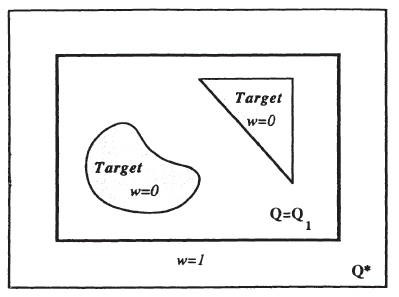
\includegraphics[scale=1]{bvpregions}
\caption{A state space divided into capture($w=0$),escape($w=1$), and regions of play($Q=Q_1$) \cite{bardi2}}
\label{bvpregions}
\end{figure}
The discretized state space is then divided into regions such as those in \Cref{bvpregions}. For this problem, $\mathscr{T}$ denotes the nodes in the target region and is a subset of the nodes in $Q$. The target region is the area in which the pursuer captures the evader. $Q_1$ is the region of play and contains all nodes in $Q$ that are not in the target region or the escape region. The escape region is denoted by $Q_2$ and may contain nodes in $Q$ and $R^M$, where $R^M$ is the boundary of the bounded state space. All the nodes in the escape region represent states in which it is assumed that the evader has avoided capture by the pursuer. A common division of the state space is to set $\mathscr{T}=$ origin, $Q_1 = Q$, and $Q_2 = R^M$. The discretization of the state space results in a discrete version of the Hamilton-Jacobi-Isaacs equation for the boundary value problem(HJD):
\begin{align}
  & w(x)  =  \sum_j\lambda_jw(x_j) && \textnormal{ if } x = \sum_j\lambda_jx_j \label{dbvp1} \\
  & w(x_i)  =  \gamma\underset{b}{\operatorname{max \textnormal{ } }}\underset{a}{\operatorname{min \textnormal{ }}} w(x_i +hf(x_i,a,b))+1-\gamma && \textnormal{ if } x_i \in Q\textbackslash \mathscr{T} \label{dbvp2} \\
  & w(x_i) = 1 && \textnormal{ if } x_i \in Q_2\textbackslash Q \label{dbvp3} \\
  & w(x_i) = 0 && \textnormal{ if } x_i \in (\mathscr{T} \cap Q) \cup (R^M \textbackslash Q_2) \label{dbvp4} \\
  & \textnormal{where } \gamma = e^{-h} \label{dbvp5}
\end{align}    


Since the HJD is completely discretized into a finite number of states, it can easily be seen that by using dynamic programming $w(x_i)$ can be solved for any initial condition $x_0$. Furthermore, in a previous paper by Bardi and Soravia, "Hamilton-Jacobi equations with singular boundary conditions on a free boundary and applications to differential games,"\cite{bardi1} they are able to prove that the continuous boundary value problem:
\begin{equation}\label{eqn1}
v(x) + \underset{b \in B }{\operatorname{min \textnormal{ }}}\underset{a \in A}{\operatorname{max}}{-f(x,a,b)\cdot Dv(x)-1}=0 \textnormal{ in } R^M\textbackslash \mathscr{T} \equiv \mathscr{T}^C,
\end{equation}
has a unique bounded viscosity solution $v$ that meets the natural Dirichlet boundary condition:
\begin{equation}\label{eqn2}
v(x) = 0 \textnormal{ for } x \in \delta \mathscr{T},
\end{equation}
if $v$ is continuous. They are further able to characterize this viscosity solution as:
\begin{equation}\label{eqn3}
v(x) \equiv 
\begin{cases}
1-e^{-\textnormal{T}(x)}, & \textnormal{ if T}(x) < + \infty,\\
1, & \textnormal{ if T}(x) = + \infty.
\end{cases}
\end{equation}
Denoting $w_n$ as the unique solution to the HJD, $Q^n$ as the discretization of the state space, $h_n$ as the time step, and $|f(x_i,a,b)| \leq M_f$, Bardi, Falcone, and Soravia show that $w_n$ will converge to the unique bounded viscosity solution $v$ as $Q^n$ and $h_n$ become infinitely small. This is presented in: 
\begin{theorem}[Convergence of Bounded Viscosity Solution \cite{bardi2}]\label{dbvpt}
Assume $|f(x,a,b)-f(y,a,b)| \leq L|x-y|$ for all $x,y,a,b$; $|f(x_i,a,b)| \leq M_f$ for all $x \in \delta$T and all $a,b$; T is the closure of an open set with Lipschitz boundary ; $(Q^n,h_n)$ is an admissible sequence ; there is a bounded continuous viscosity solution $v$ of \Cref{eqn1,eqn2}. Then $w_n$ converge to $v$ as $n \rightarrow \infty$, uniformly on any compact set of $R^M$.   
\end{theorem}
In order to demonstrate the ability of these discretized boundary value problems, Bardi, Falcone, and Soravia implemented the system of \Cref{dbvp1,dbvp2,dbvp3,dbvp4,dbvp5} with simple one-dimensional pursuit-evasion games. The results of these games can be seen in \Cref{bvpresults}.\cite{bardi2}
\begin{figure}[h!]
\centering
\begin{subfigure}[t]{0.475\textwidth}
	\centering
	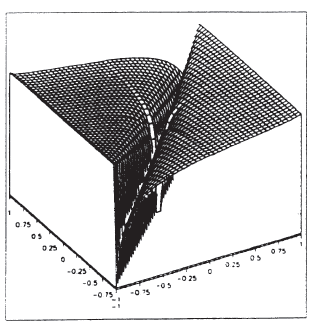
\includegraphics[width=\textwidth]{bvpresult1}
	\caption{Approximate value function when $v_1 = 1$, $v_2 = 1$}
	\label{bvpresult1}
\end{subfigure}
\hfill
\begin{subfigure}[t]{0.475\textwidth}
	\centering
	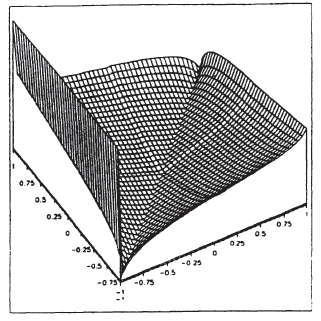
\includegraphics[width=\textwidth]{bvpresult2}
	\caption{Approximate value function when $v_1 = 5$, $v_2 = 1$}
	\label{bvpresult2}
\end{subfigure}
\caption{Results for one-dimensional pursuit-evasion games \cite{bardi2}}
\label{bvpresults}
\end{figure}
   
Bardi, Falcone, and Soravia's discrete method of solving pursuit-evasion games offers a number of advantages and disadvantages. As given in \Cref{dbvpt}, their method has the advantage of being mathematically sound. Since they focus on solving pursuit-evasion games with continuous viscosity solutions, they are able to prove that these games converge to a guaranteed optimal solution under certain conditions. A major disadvantage that arises from this is that the method does not guarantee convergence to an optimal solution if barriers or other factors that break the continuity of the solution exist. The restriction to a compact state space can also be problematic. Given too small of a state space the method might omit potential solutions that require leaving the state space. For example, given a pursuer with greater speed but less maneuverability it has been shown that an optimal strategy may require the pursuer to increase the distance between itself and the evader before making the capture \cite{isaacs}. Under these conditions the discrete boundary value problem may determine that under optimal control the evader can escape while in reality the pursuer has an optimal strategy that results in the capture of the evader.

The simple solution to this problem is to increase the state space. However, as the state space increases either the discretization must decrease or the number of discrete state nodes increases. This can be problematic when the state space encompasses a number of dimensions $d$ that are evenly discretized into $n$ states resulting in a total of $n^d$ state nodes. In this case, any increase in the discretization of the state space results in order $d$ polynomial growth of the state nodes. When $d$ is large this is called the curse of dimensionality. Bardi, Falcone, and Soravia tested their algorithm for solving discrete boundary value problems on a state space composed of 1849 nodes. Given a state of just the x and y position of both the pursuer and the evader with each dimension discretized into twenty discrete values would result in a state space with a size of $20^4 = 1.6 \times 10^5$. Because of this further methods must be used to efficiently solve pursuit-evasion games. 

\section{RRT*}
Besides dynamic programming, other methods have been used to solve pursuit-evasion games. Sertac Karaman and Emilio Frazzoli use a special version of Rapidly-exploring Random Tree (RRT) algorithm called $\textnormal{RRT}^*$ and Stackelberg strategies to solve pursuit-evasion games in "Incremental Sampling-Based Algorithms for a Class of Pursuit-Evasion Games" \cite{karaman}. Due to the edge updating scheme used by $\textnormal{RRT}^*$, this method can be effectively used as a shortest path algorithm. Karaman and Frazzoli use this method to determine the shortest path to a goal region for an evader without being caught by multiple pursuers.

The $\textnormal{RRT}^*$ algorithm is the cornerstone to Karaman and Frazzoli's ability to solve this pursuit-evasion problem. This algorithm can be used to determine the optimal shortest path as the number of iterations it is run for approaches infinity. To start the algorithm, a tree $G$ composed of vertices and edges $(V,E)$ is initialized to a single vertex at the vehicle's initial position $z_{init}$. Next, a single point $z_{rand}$ is randomly sampled from the entirety of the continuous state space $X$. The nearest vertex $z_{nearest}$ to $z_{rand}$ is then determined. A trajectory $x_{new}$ between $z_{nearest}$ and $z_{init}$ is formulated along with the controls $u_{new}$ required to traverse the trajectory. If $z_{nearest}$ can be reached within some time $t_{max}$ then $t_{new}$ takes on the time required to traverse $x_{new}$ to reach $z_{init}$. Otherwise, $t_{new} = t_{max}$. A new vertex $z_{new}$ is now determined by following $x_{new}$ for $t_{new}$. If $x_{new}$ is obstacle free, then $z_{new}$ is added to the list of vertices $V$. 

If the edge between $z_{new}$ and $z_{nearest}$ was added to the list of edges $E$, then this step along with the preceding steps would characterize the RRT algorithm. However, what makes $\textnormal{RRT}^*$ special is the next two steps in determining edges. First, within some radius all the nearby vertices, $Z_{near}$, to $z_{new}$ are used to determine the edge which reaches $z_{new}$ in optimal time $c_{min}$. The edge between $z_{new}$ and the optimal vertex $z_{min}$ is then added to $E$. Secondly, all the nearby vertices that are not $z_{min}$ are tested to determine if they can be reached in a more optimal time through $z_{new}$. If this is the case then the edge between $z_{new}$ and the vertex $z_{near}$ is added to $E$ while the edge between $z_{near}$ and the original parent, or vertex that connected $z_{near}$ to $z_{init}$, is removed. This algorithm can be viewed in detail in \Cref{RRTalg,extend}. \cite{karaman} 
  
The last two steps of $\textnormal{RRT}^*$ are especially important because they convey upon the algorithm the eventuality of optimality that is not present in RRT. If the vertices defined as nearby are all the vertices within a ball of volume $\gamma \dfrac{\textnormal{log }n}{n}$ centered at $z_{new}$ and  $n = |V|$, then $\textnormal{RRT}^*$ will converge to optimality under the conditions of \Cref{RRTopt} given that $\mu(\cdot)$ is the Lebesgue measure.
\begin{theorem}[Asymptotic Optimality of $\textnormal{RRT}^*$ \cite{karaman}]\label{RRTopt}
If $\gamma > 2^d(1+1/d)\mu(X \backslash Xi_{obs})$, the event that for any vertex $z$ that is in the tree in some finite iteration $j$ the $\textnormal{RRT}^*$ algorithm converges to a trajectory that reaches $z$ optimally, i.e., in time $T^*(z)$, occurs with probability one. Formally,
\begin{align*}
&\mathbb{P}(\{\lim\limits_{i \rightarrow \infty}T(z)[i+j] = T^*(z),   \forall z \in V[j]\}) = 1, && \forall j \in \mathbb{N}.
\end{align*}   
\end{theorem}

\begin{algorithm}
\caption{$\textnormal{RRT}^*$ \cite{karaman}}\label{RRTalg}
\begin{algorithmic}[1]
	\State $V \leftarrow {z_{init}}; E \leftarrow \null; i \leftarrow 0;$
	\While{ $i<N$} \do{}
		\State $G \leftarrow (V,E);$
		\State $z_{rand} \leftarrow \textnormal{Sample}(i);$
		\State $(V,E,z_{new}) \leftarrow \textnormal{Extend}(G,z_{rand});$
		\State $i \leftarrow i +1;$
	\EndWhile
\end{algorithmic}
\end{algorithm} 

\begin{algorithm}
\caption{$\textnormal{Extend}(G,z)$ \cite{karaman}}\label{extend}
\begin{algorithmic}[1]
	\State $V' \leftarrow V; E' \leftarrow E;$
	\State $z_{nearest} \leftarrow \textnormal{Nearest}(G,z);$
	\State $(x_{new},u_{new},t_{new}) \leftarrow \textnormal{Steer}(z_{nearest},z); z_{new} \leftarrow x_{new}(t_{new});$
	\If{ $\textnormal{ObstacleFree}(x_{new})$}
		\State $V' \leftarrow V' \cup \{z_{new}\};$
		\State $z_{min} \leftarrow z_{nearest}; c_{min} \leftarrow T(z_{new});$
		\State $Z_{nearby} \leftarrow \textnormal{Near}(G,z_{new},|V|);$
		\For{ all $z_{near} \in Z_{nearby}$} \do{}
			\State $(x_{near},u_{near},t_{near}) \leftarrow \textnormal{Steer}(z_{near},z_{new});$
			\If{ObstacleFree$(x_{near})$ and $x_{near}(t_{near})=z_{new}$ and $T(z_{near}) + \textnormal{EndTime}(x_{near})< T(z_{new})$}
				\State $c_{min} \leftarrow T(z_{near})+\textnormal{EndTime}(x_{near});$
				\State $z_{min} \leftarrow z_{near};$
			\EndIf
		\EndFor
		\State $E' \leftarrow E' \cup \{(z_{min},z_{new})\};$
		\For{ all $z_{near} \in Z_{nearby} \ \{z_{min}\}$} \do{}
			\State $(x_{near},u_{near},t_{near}) \leftarrow \textnormal{Steer}(z_{new},z_{near});$
			\If{ ObstacleFree$(x_{near})$ and $x_{near}(t_{near})=z_{near}$ and $T(z_{near})>T(z_{new})+\textnormal{EndTime}(x_{near})$}
				\State $z_{parent} \leftarrow \textnormal{Parent}(z_{near});$
				\State $E' \leftarrow E' \ \{(z_{parent},z_{near})\};E' \leftarrow E' \cup \{(z_{new},z_{near})\};$
			\EndIf
		\EndFor
		\Else
			\State $z_{new} = \textnormal{NULL};$
	\EndIf
	\State
	\Return $G' = (V',E',z_{new})$
\end{algorithmic}
\end{algorithm}

Karaman and Frazzoli further apply the $\textnormal{RRT}^*$ algorithm to solve pursuit-evasion games. In order to do this, they implement a Stackelberg strategy in which the evader first choses its controls and then the pursuers  follow the evader by choosing their controls to counter the strategy of the evader. These types of strategies provide for a worst case scenario for the evader. Therefore, if the $\textnormal{RRT}^*$ pursuit-evasion algorithm finds a winning strategy for the evader this strategy will always result in a win for the evader no matter what strategy the pursuers choose.

The pursuit-evasion algorithm modifies upon $\textnormal{RRT}^*$ by creating trees for both the evader $G_e$ and the pursuer $G_p$. Besides creating two separate trees, the pursuit-evasion algorithm also checks all the nearby vertices of the other player. If the new evader vertex can be reached in less time by a nearby pursuer vertex or a new pursuer vertex can reach nearby evader vertices in less time, then those evader vertices along with their connecting edges are removed from $G_e$. This algorithm can be examined in detail in \Cref{RRTpealg}.\cite{karaman}
         
\begin{algorithm}
\caption{Pursuit-Evasion $\textnormal{RRT}^*$ \cite{karaman}}\label{RRTpealg}
\begin{algorithmic}[1]
	\State $V_e \leftarrow {x_{e,init}}; E_e \leftarrow \null; V_p \leftarrow {x_{p,init}}; E_p \leftarrow \null; i \leftarrow 0;$
	\While{ $i<N$} \do{}
		\State $G_e \leftarrow (V_e,E_e);G_p \leftarrow (V_p,E_p)$
		\State $z_{e,rand} \leftarrow \textnormal{Sample}_e(i);$
		\State $(V_e,E_e,z_{e,new}) \leftarrow \textnormal{Extend}_e(G_e,z_{e,rand});$
		\If{$z_{e,new} \neq \textnormal{NULL}$}
			\State $Z_{p,near} \leftarrow \textnormal{NearCapture}_e(G_p,z_{e,new},|V_p|);$
			\For{ all $z_{p,near} \in Z_{p,near}$} \do{}
				\If{Time$(z_{p,near}) \leq \textnormal{Time}(z_{e,new})$}
					\State Remove$(G_e,z_{e,new});$
				\EndIf
			\EndFor
		\EndIf
		\State $z_{p,rand} \leftarrow \textnormal{Sample}_p(i);$
				\State $(V_p,E_p,z_{p,new}) \leftarrow \textnormal{Extend}_p(G_p,z_{p,rand});$
				\If{$z_{p,new} \neq \textnormal{NULL}$}
					\State $Z_{e,near} \leftarrow \textnormal{NearCapture}_p(G_e,z_{p,new},|V_e|);$
					\For{ all $z_{e,near} \in Z_{e,near}$} \do{}
						\If{Time$(z_{p,new}) \leq \textnormal{Time}(z_{e,near})$}
							\State Remove$(G_e,z_{e,near});$
						\EndIf
					\EndFor
				\EndIf
		\State $i \leftarrow i +1;$
	\EndWhile
	\State
	\Return $G_e,G_p$
\end{algorithmic}
\end{algorithm}

In order to demonstrate the abilities of the pursuit-evasion $\textnormal{RRT}^*$, Karaman and Frazzoli implement this algorithm on two different examples. In the first example, simplified dynamics are used. For the evader, the dynamics are:
\begin{equation*}
\dfrac{d}{dt}x_e(t) = \dfrac{d}{dt}\left[ \begin{array}{c}
x_{e,1}(t) \\
x_{e,2}(t) \end{array} \right] = u_e(t) = \left[ \begin{array}{c}
u_{e,1}(t) \\
u_{e,2}(t) \end{array} \right],
\end{equation*}
with $\|u_e(t)\|_2 \leq 1$, while the pursuers have the following dynamics:
\begin{equation*}
\dfrac{d}{dt}x_p(T) = \dfrac{d}{dt}\left[ \begin{array}{c}
x_{p_1}(t) \\
x_{p_2}(t) \\
x_{p_3}(t) \end{array} \right] = \dfrac{d}{dt}\left[ \begin{array}{c}
x_{p_1,1}(t) \\
x_{p_1,2}(t) \\
x_{p_2,1}(t) \\
x_{p_2,2}(t) \\
x_{p_3,1}(t) \\
x_{p_3,1}(t) \end{array} \right] =
\left[ \begin{array}{c}
u_{p_1}(t) \\
u_{p_2}(t) \\
u_{p_3}(t) \end{array} \right] = \left[ \begin{array}{c}
u_{p_1,1}(t) \\
u_{p_1,2}(t) \\
u_{p_2,1}(t) \\
u_{p_2,2}(t) \\
u_{p_3,1}(t) \\
u_{p_3,1}(t) \end{array} \right],
\end{equation*}                   
with $\|u_{p_1}(t)\|_2 \leq 1$, $\|u_{p_2}(t)\|_2 \leq 0.5$, and $\|u_{p_3}(t)\|_2 \leq 0.5$. The second example uses Dubins dynamics where the evader can be modeled by the following differential equations:
\begin{align*}
& x_e(t) = [x_{e,1}(t),x_{e,2}(t),x_{e,3}(t),x_{e,4}(t),x_{e,5}(t)]^T , & \\
& f(x_e(t),u_e(t)) = [v_e \textnormal{cos}(x_{e,3}(t)),v_e \textnormal{sin}(x_{e,3}(t)),u_{e,1}(t),x_{e,5}(t),u_{e,2}(t)]^T , &\\
& \dot{x}_e(t) = f(x_e(t),u_e(t)), & \\
& v_e = 1, |u_{e,1}(t)| \leq 1, |u_{e,2}(t)| \leq 1, |x_{e,5}| \leq 1. &
\end{align*} 
The pursuer also follows Dubins dynamics with the following differential equations:
\begin{align*}
& x_p(t) = [x_{p,1}(t),x_{p,2}(t),x_{p,3}(t),x_{p,4}(t),x_{p,5}(t)]^T , & \\
& f(x_p(t),u_p(t)) = [v_p \textnormal{cos}(x_{p,3}(t)),v_p \textnormal{sin}(x_{p,3}(t)),u_{p,1}(t),x_{p,5}(t),u_{p,2}(t)]^T , &\\
& \dot{x}_p(t) = f(x_p(t),u_p(t)), & \\
& v_p = 2, |u_{p,1}(t)| \leq 1/3, |u_{p,2}(t)| \leq 1, |x_{p,5}| \leq 1. &
\end{align*}
The results of these examples can be seen in \Cref{rrtfig,rrtobsfig,rrtdubinsfig}.\cite{karaman}   
\begin{figure}
\centering
\begin{subfigure}[b]{0.475\textwidth}
	\centering
	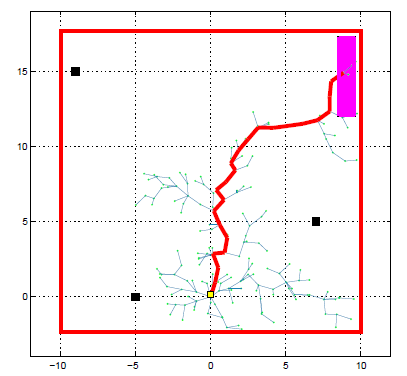
\includegraphics[width=\textwidth]{rrt500}
	\caption{500 iterations }
	\label{rrt500}
\end{subfigure}
\hfill
\begin{subfigure}[b]{0.475\textwidth}
	\centering
	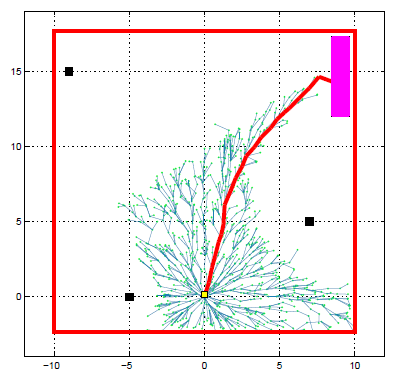
\includegraphics[width=\textwidth]{rrt3000}
	\caption{3000 iterations}
	\label{rrt3000}
\end{subfigure}
\vskip\baselineskip
\begin{subfigure}[b]{0.475\textwidth}
	\centering
	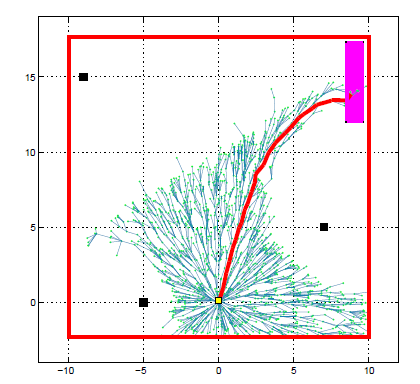
\includegraphics[width=\textwidth]{rrt5000}
	\caption{5000 iterations}
	\label{rrt5000}
\end{subfigure}
\quad
\begin{subfigure}[b]{0.475\textwidth}
	\centering
	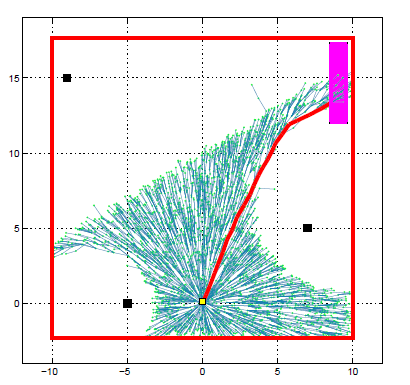
\includegraphics[width=\textwidth]{rrt10000}
	\caption{10000 iterations}
	\label{rrt10000}
\end{subfigure}
\caption{Pursuit-Evasion $\textnormal{RRT}^*$ at various iterations \cite{karaman}}
\label{rrtfig}
\end{figure}

\begin{figure}
\centering
\begin{subfigure}[b]{0.475\textwidth}
	\centering
	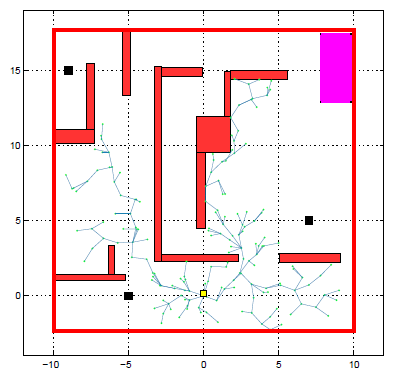
\includegraphics[width=\textwidth]{rrtobs500}
	\caption{500 iterations}
	\label{rrtobs500}
\end{subfigure}
\hfill
\begin{subfigure}[b]{0.475\textwidth}
	\centering
	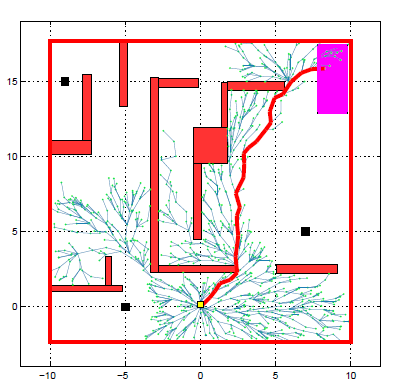
\includegraphics[width=\textwidth]{rrtobs3000}
	\caption{3000 iterations}
	\label{rrtobs3000}
\end{subfigure}
\vskip\baselineskip
\begin{subfigure}[b]{0.475\textwidth}
	\centering
	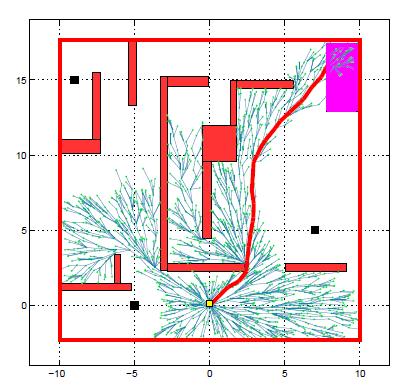
\includegraphics[width=\textwidth]{rrtobs5000}
	\caption{5000 iterations}
	\label{rrtobs5000}
\end{subfigure}
\quad
\begin{subfigure}[b]{0.475\textwidth}
	\centering
	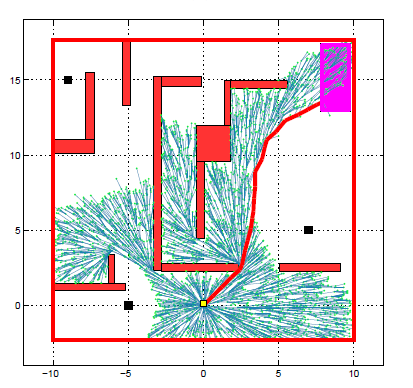
\includegraphics[width=\textwidth]{rrtobs10000}
	\caption{10000 iterations}
	\label{rrtobs10000}
\end{subfigure}
\caption{Pursuit-Evasion $\textnormal{RRT}^*$ in a field with obstacles at various iterations\cite{karaman}}
\label{rrtobsfig}
\end{figure}

\begin{figure}
\centering
\begin{subfigure}[b]{0.475\textwidth}
	\centering
	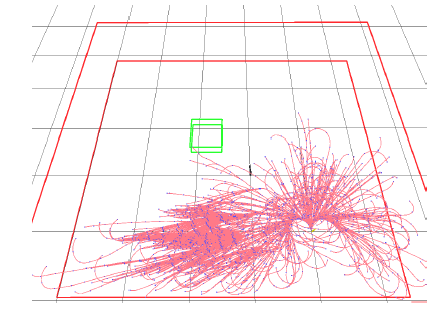
\includegraphics[width=\textwidth]{rrtdubins}
	\caption{Pursuit-Evasion $\textnormal{RRT}^*$ run for 3000 iterations}
	\label{rrtdubins}
\end{subfigure}
\hfill
\begin{subfigure}[b]{0.475\textwidth}
	\centering
	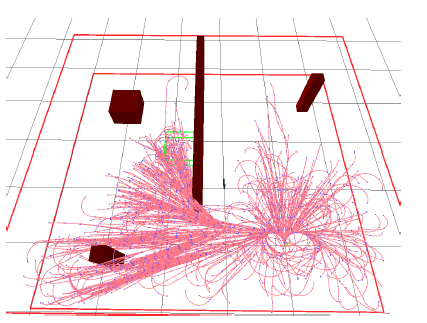
\includegraphics[width=\textwidth]{rrtobsdubins}
	\caption{Pursuit-Evasion $\textnormal{RRT}^*$ run for 3000 iterations in a field with obstacles}
	\label{rrtobsdubins}
\end{subfigure}
\caption{Pursuit-Evasion $\textnormal{RRT}^*$ on a problem with Dubins dynamics \cite{karaman}}
\label{rrtdubinsfig}
\end{figure}

Just as with dynamic programming, there are numerous advantages and disadvantages to using $\textnormal{RRT}^*$ to solve pursuit-evasion games. The computational speed of $\textnormal{RRT}^*$ is the biggest advantage to using this algorithm. 10000 iterations of the simple dynamics example were computed in about 3 seconds, while 3000 iterations of the Dubins dynamics example were computed in about 20 seconds \cite{karaman}. Unlike the dynamic programming method presented in \Cref{1dbvp}, $\textnormal{RRT}^*$ also handles obstacles very well as can be seen in \Cref{rrtobsfig,rrtobsdubins}. 

The major disadvantage of $\textnormal{RRT}^*$ is in its inability to handle sub-optimality very well. If either the pursuer or evader ends up taking suboptimal actions, the results of the $\textnormal{RRT}^*$ algorithm could be completely useless. For example, suppose that the evader moves into the region of potential pursuer capture by accident. However, the pursuer is elsewhere expecting evader optimal control. In this case the only way to determine a new path for the evader is to recompute the entire solution.             
%% This is an example first chapter.  You should put chapter/appendix that you
%% write into a separate file, and add a line \include{yourfilename} to
%% main.tex, where `yourfilename.tex' is the name of the chapter/appendix file.
%% You can process specific files by typing their names in at the 
%% \files=
%% prompt when you run the file main.tex through LaTeX.
\chapter{Tensor-Train Decomposition}\label{chp:TT}

One method of handling the curse of dimensionality is to reduce the number of states that must be examined. If a problem has a low-rank representation, tensor-train decomposition may be used to reduce the number of states employed to compute the solution to a problem \cite{Osel3}. Tensor-train decomposition, as outlined in Oseledets's "Tensor-train decomposition" and "TT-cross approximation for multidimensional arrays," takes advantage of the structure of tensors to reduce the state space \cite{Osel1,Osel2}. This method takes advantage of single value decomposition (SVD) to create compact tensors. This chapter provides a description of tensors in general. In particular, the chapter explains how tensor-train decomposition works, and under what circumstances this method works best. Finally, a series of methods for maintaining low-rank will be provided along with the TT-SVD algorithm.

\section{Tensor-Train Decomposition}
Tensors are another way of representing a multidimensional array. Given such an array or tensor \textbf{A}, the element at $A(i_1,i_2,...,i_d)$, where $d$ is the dimensionality of the tensor and $i_j$ is the $i^{th}$ entry of the $j^{th}$ dimension of the tensor, can be given by:
\begin{equation}\label{eqn4}
A(i_1,...,i_d) = \sum_{\alpha=1}^{r}U_1(i_1,\alpha)U_2(i_2,\alpha)...U_d(i_d,\alpha).
\end{equation}
The $d$ matrices $U_k = [U_k(i_k,\alpha)]$ are called canonical factors and the value $r$ is the tensor rank. The tensor rank represents the minimal number of summands required to represent the entire tensor \textbf{A} in the form of \Cref{eqn4}.

A tensor \textbf{B} can be approximated with a tensor-train \textbf{A} created from the product of a series of matrices:
\begin{equation}\label{tensaprox}
A(i_1,i_2,...,i_d) = G_1(i_1)G_2(i_2)...G_d(i_d).
\end{equation}
$G_k(i_k)$, also called a tensor core, is an $r_{k-1} \times r_k$ matrix where $r_0 = r_d=1$ is imposed. These tensor cores can also be represented by a three-dimensional array of size $r_{k-1} \times n_k \times r_k$ that has elements $G_k(\alpha_{k-1},i_k,\alpha_k)= G_k(i_k)_{\alpha_{k-1},\alpha_k}$. Therefore any individual element of a tensor-train can be calculated by:
\begin{equation}\label{eqn5}
A(i_1,...,i_d) = \sum_{\alpha_0,...,\alpha_{d-1},\alpha_d}G_1(\alpha_0,i_1,\alpha_1)G_2(\alpha_1,i_2,\alpha_2)...G_d(\alpha_{d-1},i_d,\alpha_d)
\end{equation}
As can be seen in \Cref{eqn5}, in order to compute the individual elements of the tensor all the tensor cores are multiplied and then summed over the auxiliary indices $a_k$. It is from this process that the decomposition gets the name tensor-train. Tensor-train decomposition makes it possible to represent all elements in the tensor \textbf{A} with $d$ three-dimensional arrays \cite{Osel1}.
 
Since the size of the tensor cores are determined by ranks $r_k$, determining these ranks are pivotal to the compressibility of tensor-train decomposition. The rank $r_k$ is dependent on the rank of the $k^{th}$ unfolding matrix $A_k$ which has the form:
\begin{equation}\label{unfold}
A_k = A_k(i_1,...,i_k;i_{k+1},...,i_d) = A(i_1,...,i_d).
\end{equation}
These unfolding matrices can be determined by the MATLAB reshape function as such:
\begin{equation*}
A_k = \textnormal{reshape} (\textbf{A},\prod_{s=1}^{k}n_s,\prod_{s=k+1}^{d}n_s).
\end{equation*}
By determining the rank of these unfolding matrices, a bound on the tensor-train ranks can be determined with respect to \Cref{ttranks} \cite{Osel1}.
\begin{theorem}[Bound on TT-Ranks \cite{Osel1}]\label{ttranks}
If for each unfolding matrix $A_k$ of form \ref{unfold} of a d-dimensional tensor \textbf{A}
\begin{equation*}
\textnormal{rank }A_k = r_k, 
\end{equation*}
then there exists a decomposition \ref{eqn5} with TT-ranks not higher than $r_k$.
\end{theorem}

\section{Methods of Maintaining Low Order}
Given certain tensors it may be the case that the unfolding matrices do not meet the low rank requirements of tensor-train decomposition. The unfolding matrices can be replaced by approximate low rank unfolding matrices $R_k$ such that:
\begin{equation}\label{eqn6}
A_k = R_k + E_k,\textnormal{rank } R_k = r_k, \| E_k \| = \varepsilon_k, k = 1,...,d-1.
\end{equation}
This results in a new tensor \textbf{B} where the norm of the difference between the new tensor and the old tensor is bounded by an error constant as given by:
\begin{theorem}[TT Approximation \cite{Osel1}]\label{ttaprox}
Suppose that the unfoldings $A_k$ of the tensor \textbf{A} satisfy \ref{eqn6}. Then TT-SVD computes a tensor \textbf{B} in the TT-format with TT-ranks $r_k$ and
\begin{equation*}
\| \textbf{A}-\textbf{B}\| \leq \sqrt{\sum_{k=1}^{d-1}\varepsilon_k^2}.
\end{equation*}    
\end{theorem}
The results of \Cref{ttaprox} can be used to create a tensor in TT-format as detailed in \Cref{ttsvd}.

\begin{algorithm}
\caption{TT-SVD \cite{Osel1}}\label{ttsvd}
\begin{algorithmic}[1]
	\Require $d$-dimensional tensor \textbf{A}; Prescribed accuracy $\varepsilon$.
	\Ensure Cores $G_1,...,G_d$ of the TT-approximation \textbf{B} to \textbf{A} in the TT-format with TT-ranks $\hat{r_k}$ equal to the $\delta$-ranks of the unfoldings $A_k$ of \textbf{A}, where $\delta = \dfrac{\varepsilon}{\sqrt{d-1}}\|A\|_F.$
	\Statex The computed approximation satisfies
	\begin{equation*}
	\| \textbf{A}-\textbf{B}\|_F \leq \varepsilon\|\textbf{A}\|_F.
	\end{equation*} 
	\State \{Initialization\}
	\Statex	Compute truncation parameter $\delta = \dfrac{\varepsilon}{\sqrt{d-1}}\|A\|_F.$ 
	\State Temporary tensor: $\textbf{C}=\textbf{A}, r_0 = 1.$
	\For{ $k = 1 \textnormal{ to } d-1 $} \do{}
		\State $C:= \textnormal{reshape} (C,[r_{k-1}n_k,\dfrac{\textnormal{numel}(C)}{r_{k-1}n_k}]).$
		\State Compute $\delta$-truncated SVD: $C = USV + E, \|E\|_F \leq \delta, r_k = \textnormal{rank}_\delta(C).$
		\State New core: $G_k := \textnormal{reshape}(U,[r_{k-1},n_k,r_k]).$
		\State $C:=SV^T.$
	\EndFor
	\State $G_d =C$
	\State Return tensor \textbf{B} in TT-format with cores $G_1,...,G_d$.
\end{algorithmic}
\end{algorithm}

The largest benefit of tensor-trains is that they greatly reduce the complexity of high-dimensional calculations. Generally these computations have complexity that is linear with dimension and polynomially with rank. However, many of these tensor-train computations have the unfortunate effect of increasing the rank of the final tensor-train. For example, adding two tensor-trains with the same rank takes next to no computations but doubles the number of ranks in the resulting tensor-train. Taking the scalar product of two tensor-trains takes $O(dnr^4)$ computations but results in $O(r^2)$ ranks. In order to keep the tensor-train low-rank, TT-rounding can be used to create a new tensor $\textbf{B}$ with $\delta$-ranks such that $\delta = \dfrac{\varepsilon}{\sqrt{d-1}}\| A\|$. This new approximation maintains an $\varepsilon$-level accuracy and only requires $O(dnr^2+dr^4)$ computations:
\begin{equation}
\| \textbf{A}-\textbf{B}\| \leq \varepsilon \| \textbf{A} \|.
\end{equation}
A detailed explanation for TT-rounding can be found in \Cref{ttround} \cite{Osel1}.
\begin{algorithm}
\caption{TT-Rounding \cite{Osel1}}\label{ttround}
\begin{algorithmic}[1]
	\Require $d$-dimensional tensor \textbf{A} in the TT-format; Required accuracy $\varepsilon$.
	\Ensure \textbf{B} in the TT-format with TT-ranks $\hat{r_k}$ equal to the $\delta$-ranks of the unfoldings $A_k$ of \textbf{A}, where $\delta = \dfrac{\varepsilon}{\sqrt{d-1}}\|A\|_F.$ The computed approximation satisfies
	\begin{equation*}
	\| \textbf{A}-\textbf{B}\|_F \leq \varepsilon\|\textbf{A}\|_F.
	\end{equation*}
	\State Let $G_k, k = 1,...,d,$ be cores of \textbf{A}. 
	\State \{Initialization\}
	\Statex	Compute truncation parameter $\delta = \dfrac{\varepsilon}{\sqrt{d-1}}\|A\|_F.$
	\State \{Right-to-left orthogonalization\} 
	\For{ $k = d \textnormal{ to 2 step}-1 $} \do{}
		\State $[G_k(\beta_{k-1};i_k\beta_k),R(\alpha_{k-1},\beta_{k-1})] := QR_{rows}(G_k(\alpha_{k-1};i_k\beta_k)).$
		\State $G_{k-1} := G_k \times_3 R$
	\EndFor
	\State \{Compression of the orthogonalized representation\}
	\For{ $k = 1 \textnormal{ to }d-1 $} \do{}
		\State \{Compute $\delta$-truncated SVD\}
		\Statex $[G_k(\beta_{k-1}i_k;\gamma_k),\Lambda,V(\beta_k,\gamma_k)] := SVD_\delta[G_k(\beta_{k-1}i_k;\beta_k)].$
		\State $G_{k+1} := G_{k+1} \times_1 (V\Lambda)^T$
	\EndFor
	\State Return $G_k, k = 1,...,d,$ as cores of \textbf{B}.
\end{algorithmic}
\end{algorithm}

Oseledets provides more detailed algorithms and further proofs in \cite{Osel1,Osel2}.
%% This is an example first chapter.  You should put chapter/appendix that you
%% write into a separate file, and add a line \include{yourfilename} to
%% main.tex, where `yourfilename.tex' is the name of the chapter/appendix file.
%% You can process specific files by typing their names in at the 
%% \files=
%% prompt when you run the file main.tex through LaTeX.
\chapter{Tensor-based Value Iteration}\label{chp:tvi}

The advantages of tensor-train decomposition have already been applied to solving optimal control problems with dynamic programming. Gorodetsky, Karaman, and Marzouk have come up with a version of value iteration that takes advantage of tensor-train decomposition in "Efficient High-Dimensional stochastic Optimal Motion Control using Tensor-Train Decomposition" \cite{Gorod}. They call this new version of value iteration Tensor-based value iteration(TVI). This chapter will begin by providing a quick background into stochastic optimal motion control for which Gorodetsky et.al designed TVI. Next, the TVI algorithm will be provided in detail. The chapter will end with an example problem Gorodetsky et. al. solved in \cite{Gorod} along with their results. 

\section{Stochastic Optimal Motion Control}
Gorodetsky, Karaman, and Marzouk focus on problems of stochastic optimal motion control. While deterministic pursuit-evasion games have many similarities to problems of this type, a brief explanation will be given for problems of stochastic optimal motion control in order to fully appreciate the results of TVI when applied to these problems. In problems of stochastic optimal motion control some system has the differential form:
\begin{equation}\label{eqn7}
dx(t) = b(x(t),u(t))dt + F(x(t),u(t))dw(t),
\end{equation}
in which $d,d_u,d_w \in Z_+, X \subset R^d$ and $U \subset R^{d_u}$ are compact sets with smooth  boundaries and non-empty interiors. ${w(t):t \geq 0}$ is a $d_w$-dimensional Brownian motion defined on some probability space $(\omega, \mathscr{F},P)$, where $\omega$ is a sample space. $\mathscr{F}$ is $\sigma$-algebra, and $P$ is a probability measure while $b:X \times U \rightarrow R^d$ and $F: X \times U \rightarrow R^{d \times d_w}$ are measurable, continuous, and bounded functions as detailed in \cite{Gorod}. 

Just as with the discrete boundary value problem in \cite{bardi2}, the first step is to discretize the state space. The state space is discretized using discrete Markov Decision Processes (MDPs) that follow the local consistency conditions as given by:
\begin{theorem}[Local Consistency Conditions \cite{Gorod}]
Suppose the sequence ${M_l:l \in N}$ of MDPs and the sequence ${\Delta t_l:l \in N}$ holding times satisfy the following conditions:\\
For any sequence of inputs ${u_i^l:i \in N}$ and the resulting sequence of trajectories ${\xi_i^l: i \in N}$,
\begin{itemize}
\item for all $z \in X$, 
\begin{equation*}
\lim\limits_{l \rightarrow \infty} \Delta t_l(z) = 0,
\end{equation*}
\item for all $ z \in X$ and $v \in U$,
\begin{equation*}
\lim\limits_{l \rightarrow \infty} \dfrac{E[\xi_{i+1}^l-\xi_i^l|\xi_i^l =z,u_i^l = v]}{\Delta t_l(z)} = f(z,v),
\end{equation*}
\begin{equation*}
\lim\limits_{l \rightarrow \infty} \dfrac{Cov[\xi_{i+1}^l-\xi_i^l|\xi_i^l =z,u_i^l = v]}{\Delta t_l(z)} = F(z,v),
\end{equation*}
\end{itemize}
Then, the sequence ${(\xi_i^l,u^l):l \in N}$ of interpolations converges in distribution to $(x,u)$ that solves the integral equation with differential form given by \ref{eqn7}. Let $J_l^*$ denote the optimal cost-to-go function for the MDP $M_l$. Then, for all $z \in S$, 
\begin{equation*}
\lim\limits_{l \rightarrow \infty}|J_l^*(z)-J^*(z)| = 0.
\end{equation*}    
\end{theorem}
Given that the states are discretized to a resolution $h$, where the discrete states are ${z_i:i \in l}$, the stochastic optimal control problem can be solved using value iteration and the update function:
\begin{equation}\label{eqn8}
J_h^{k+1}(z_i)= \underset{u }{\operatorname{min }}[G(z_i,u) + \gamma_h \sum_{j}P(z_j|z_i, u)J_h^{(k)}(z_j)],
\end{equation}
in which $\gamma_h$ is the discount rate that ranges from $(0,1)$. $J_h^{(k)}$ will converge to the optimal cost-to-go function as $k \rightarrow \infty$ giving the Bellman equation:
\begin{equation}
J_h^*(z_i) = \underset{u }{\operatorname{min }}[G(z_i,u) + \gamma_h \sum_{j}P(z_j|z_i,u)J_h^*(z_j)].\cite{Gorod}
\end{equation} 
  

\section{Tensor-based Value Iteration Algorithm}

The curse of dimensionality that is inherent in this problem can be solved by applying tensor-train decomposition. Instead of using normal tensor-train decomposition, a further reduction in size can be made by applying tensor-train decomposition on the skeleton of the unfolding matrices, called tensor-train cross. The skeleton unfolding matrix $A_k$ can be written as:
\begin{equation}
A_k = A_k[:,C]A_k[I,C]^{-1}A_k[C,:],
\end{equation}
where $I$ is the set of rows where $|I| \geq r$ and $C$ is the set of columns where $|C| \geq r$. Tensor-train cross can be used to solve the tensor-based value iteration algorithm as given in \Cref{TVIalg}.
\begin{algorithm}
\caption{Tensor-based Value Iteration \cite{Gorod}}\label{TVIalg}
\begin{algorithmic}[1]
	\Require Termination criterion $\delta_{max}$; TT-cross accuracy $\epsilon$; Initial cost function $\hat{J}_h^{(0)}$
	\Ensure Residual $\delta=\|\hat{J}_h^{(k)}-\hat{J}_h^{(k-1)}\|^2<\delta_{max}$
	\State $\delta = \delta_{max} + 1$
	\State $k = 0$
	\While{ $\delta > \delta_{max}$} \do{}
		\State $\hat{J}_h^{(k+1)} = \textnormal{ TT-cross }((\ref{eqn8}),\epsilon)$
		\State $k = k+1$
		\State $\delta = \|\hat{J}_h^{(k)}-\hat{J}_h^{(k-1)}\|^2$
	\EndWhile
\end{algorithmic}
\end{algorithm}

In this algorithm, a max residual and accuracy setting are given along with an initialized guess of the cost function $\hat{J}_h^{(0)}$ in tensor-train form. The initial residual is set such that the algorithm enters the loop that continues while $\delta > \delta_{max}$. Taking as input the update function, \Cref{eqn8}, and the accuracy setting $\epsilon$, the TT-cross function returns an updated cost function that maintains the accuracy setting. Finally the iteration and residual value are updated. This algorithm continues until $\delta < \delta_{max}$. 

It is further shown in \Cref{tviae} that the error of tensor-based value iteration can be bounded.
\begin{theorem}[TVI Approximation Error \cite{Gorod}]\label{tviae}
When the proposed interpolation method are run for k iterations on a grid with resolution h, and TT-cross accuracy $\epsilon$, the number of computational operations performed by the algorithm is $O(\dfrac{kdr^3}{h})$ and the resulting approximation error satisfies:
\begin{equation*}
\| \hat{J}_j^{(k)}-J_{u_h^*}\| \leq \epsilon(\dfrac{R_{max}+\gamma}{1-\gamma})+\gamma^{k+1}\epsilon \|\tilde{J}_h^{(0)}\|+\gamma^k \|\tilde{J}_h^{(0)}-J_{u_h^*}\|.
\end{equation*}    
\end{theorem}
Where $R_{max} = \underset{u(x), x }{\operatorname{max }} r(x,u(x))$ and $\tilde{J}_h^{(k)}$ is the cost-to-go approximation of the $k^{th}$ iteration of normal value iteration.


\section{Test and Results}

Gorodetsky, Karaman, and Marzouk perform this tensor-based value iteration on a seven dimensional perching glider problem. In this problem, a glider navigates a two dimensional plane under the influence of the seven following state variables: $(x,y,\theta,\phi,v_x,v_y,\dot{\theta})$. The variables in order are the $x$ position, $y$ position, angle of attack, elevator angle, horizontal speed, vertical speed, and the angle of attacks rate of change. Elevator angle rate of change $\dot{\phi}$ is the only control variable present in this problem. The optimization problem for this perching glider problem is represented in \cite{Gorod} as:
\begin{equation}\label{eqn9}
J^*(z)= \underset{u(t) }{\operatorname{min }}E[\int_{0}^{T}\bar{x}'Q\bar{x}+ 0.1u^2dt + \bar{x}(T)'Q_f\bar{x}(T) ],
\end{equation}
\begin{eqnarray*}
\textnormal{s.t.,} &&\\
x_w & = & [x-l_w c_{\theta},y-l_w s_\theta],\\
\dot{x}_w & = & [\dot{x}+l_w \dot{\theta}s_\theta,\dot{y}-l_w \dot{\theta} c_\theta],\\
x_e & = & [x-lc_{\theta}-l_e,c_{\theta_{+\phi}},y-ls_\theta - l_e s_{\theta_{+\phi}}],\\
\dot{x}_e & = & [\dot{x}+l\dot{\theta}s_{\theta}+l_e(\dot{\theta}+u)s_{\theta_{+\phi}},\dot{y}-l\dot{\theta}c_\theta - l_e (\dot{\theta}+u) c_{\theta_{+\phi}}],\\
\alpha_w &=& \theta - \textnormal{tan}^{-1}(\dot{y}_w,\dot{x}_w), \\
\alpha_e &=& \theta + \phi -  \textnormal{tan}^{-1}(\dot{y}_e,\dot{x}_e), \\
f_w &=& \rho S_w |\dot{x}_w|^2 \textnormal{sin}(\alpha_w), \\
f_e &=& \rho S_e |\dot{x}_e|^2 \textnormal{sin}(\alpha_e), \\
m\ddot{x} &=& -f_w s_\theta - f_e s_{\theta_{+\phi}}+ Fdw, \\
m\ddot{y} &=& f_w c_\theta - f_e c_{\theta_{+\phi}}-mg+ Fdw, \\
I\ddot{\theta} &=& -f_w l_w - f_e(lc_\phi +l_e) + Fdw.
\end{eqnarray*}
In the above dynamics $\rho$ represents the air density, $m$ is the glider mass, and $I$ is the glider's moment of inertia. $S_w$ and $S_e$ are the wing and tail control surface areas respectively. The length from the center of gravity to the elevator is $l$. $l_w$ is the wing half cord and $l_e$ is the elevator half cord. Finally, $c_\gamma$ represents the cos($\gamma$) and $s_\gamma$ represents the sin($\gamma$). By uniformly discretizing each variable into 32 states, tensor-based value iteration is capable of performing value iteration on a problem with a discretized state space of $ 3.4 \times 10^{10}$ states with a maximal error of $ \epsilon = 0.1$. The resulting glide path and vertical and horizontal velocity of the optimal solution can be seen in \Cref{gorodglide}.
\begin{figure}
\centering
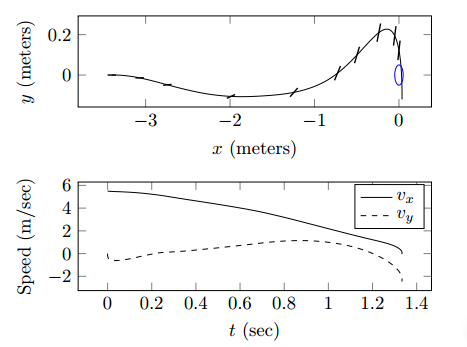
\includegraphics[scale=1]{gorodglide}
\caption{Optimal glide path with vertical and horizontal velocities \cite{Gorod}}
\label{gorodglide}
\end{figure}

The key to tensor-train value iterations success is the reduction in the number of states used. Of the $3.4 \times 10^{10}$ states making up the initial discretized state space, only about $10^6$ of these states are used as can be seen in \Cref{gorodstates}.\cite{Gorod}
\begin{figure}
\centering
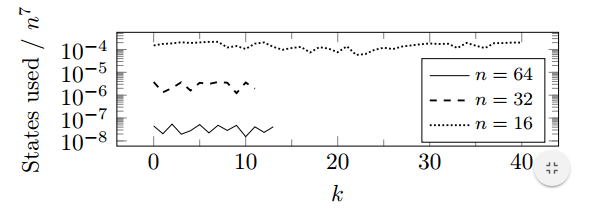
\includegraphics[scale=1]{gorodstates}
\caption{Fraction of states evaluated by TTVI in optimal glide problem \cite{Gorod}}
\label{gorodstates}
\end{figure}
%% This is an example first chapter.  You should put chapter/appendix that you
%% write into a separate file, and add a line \include{yourfilename} to
%% main.tex, where `yourfilename.tex' is the name of the chapter/appendix file.
%% You can process specific files by typing their names in at the 
%% \files=
%% prompt when you run the file main.tex through LaTeX.
\chapter{Tensor-Based Value Iteration for Pursuit-Evasion Games}\label{chp:tvipe}
Building on the work presented in \Cref{chp:tvi}, this chapter will present an algorithm that uses TVI to solve pursuit-evasion games. First, a description of the general dynamic programming problem used to model a pursuit-evasion game is given. Next, the chapter details how best response can be used along with dynamic programming to solve for the optimal control of both the pursuer and the evader. The Best Response Dynamic Programming algorithm is then be presented in detail. Finally, the chapter culminates in the presentation of the Best-Response Tensor-Train-decomposition-based Value Iteration algorithm.  

\section{Description of Problem}\label{peprobdes}
As demonstrated in \Cref{pegames}, solving pursuit-evasion games requires determining optimal control values for two or more players with opposing outcomes. In order to keep the problem as simple as possible there will be a focus on zero-sum games in which the cost function of the pursuer is the negative of the evader's: $(G_1(x) = -G_2(x))$. Although this constraint will be used throughout this thesis, it is possible to apply TVI to nonzero-sum games or even simply use predetermined controls as either the pursuer or evaders control values. Before exploring the modifications brought about by adjusting TVI for pursuit-evasion games, a description of how dynamic programming may be used with best response will be provided.

Value iteration can be modified to solve pursuit-evasion games by using a best response dynamic to solve for the optimal cost at each state. To begin with, the problem is modeled as a discounted, deterministic, shortest path problem where $\gamma$ is the discount factor. First, the state space $Z$ is discretized into evenly spaced states $z_i \in Z$ where the difference between states is $h$ just as in \cite{bardi2}. Given that $z_i$ is the current state, $u_1$ is the pursuer control, and $u_2$ is the evader control, $P(z_j|z_i,u_1,u_2) = 1$ where $z_j$ is the deterministic result of $f(z_i,u_1,u_2)$. Even if $z_j \notin z_i$, the state cost at $z_j$ can be determined by:
\begin{equation}\label{concomb}
J(z_j)  =  \sum_i\lambda_iJ(z_i),
\end{equation}
where:
\begin{equation}\label{lamb}
\lambda_i = 
\begin{cases}
\dfrac{1-|z_j-z_i|}{h}, & \forall i \textnormal{ }|\textnormal{ } |z_i-z_j|\leq h,\\
0, & \textnormal{ otherwise}.
\end{cases}
\end{equation} 
Each run of best response $K$ results in a control policy $u^K$ which is used as a constant control policy for the opponent. 

Instead of using a single update function as in \Cref{eqn8}, we model the problem as solving two separate update functions over the same state-space:
\begin{equation}\label{pbell}
J_p^{(k+1,K)}(z_i)= \underset{u_1 }{\operatorname{min }}[G(z_i,u_1,u_2^K)+\gamma J_p^{(k,K)}(z_j|z_i,u_1,u_2^K)],
\end{equation}
\begin{equation}\label{ebell}
J_e^{(k+1,K)}(z_i)= \underset{u_2 }{\operatorname{max }}[G(z_i,u_1^K,u_2)+\gamma J_e^{(k,K)}(z_j|z_i,u_1^K,u_2)].
\end{equation} 
By running the update functions until $k \rightarrow \infty$, the optimal value function is achieved for a given opponents control policy $u^K$:
\begin{equation}\label{popt}
J_p^{(*,K)}(z_i)= \underset{u_1 }{\operatorname{min }}[G(z_i,u_1,u_2^K)+\gamma J_p^{(*,K)}(z_j|z_i,u_1,u_2^K)],
\end{equation}
\begin{equation}\label{eopt}
J_e^{(*,K)}(z_i)= \underset{u_2 }{\operatorname{max }}[G(z_i,u_1^K,u_2)+\gamma J_e^{(*,K)}(z_j|z_i,u_1^K,u_2)].
\end{equation}
The optimal value functions can then be used to solve for the optimal control values $u_1^{(*,K)}$ and $u_2^{(*,K)}$:
\begin{equation}\label{pcont}
u_1^{(*,K)}(z_i)= \underset{u_1 }{\operatorname{arg min }}[G(z_i,u_1,u_2^K)+\gamma J_p^{(*,K)}(z_j|z_i,u_1,u_2^K)],
\end{equation}
\begin{equation}\label{econt}
u_2^{(*,K)}(z_i)= \underset{u_2 }{\operatorname{arg max }}[G(z_i,u_1^K,u_2)+\gamma J_e^{(*,K)}(z_j|z_i,u_1^K,u_2)].
\end{equation}  

\section{Best Response}
In "Dynamic Noncooperative Game Theory", Tamer Basar and Geert Olsder prove that under certain conditions the best response dynamic will converge at a saddle point or Nash equilibrium. A major condition is that the value function $V$ satisfies the partial differential equation:
\begin{eqnarray}\label{pde}
-\dfrac{\delta V}{\delta t} & = & \underset{u_1 \in S_1 }{\operatorname{min }}\underset{u_1 \in S_2 }{\operatorname{max }}[\dfrac{\delta V}{\delta x}f(t,x,u_1,u_2)+g(t,x,u_1,u_2)] \\
                            & = & \underset{u_1 \in S_2 }{\operatorname{max }}\underset{u_1 \in S_1 }{\operatorname{min }}[\dfrac{\delta V}{\delta x}f(t,x,u_1,u_2)+g(t,x,u_1,u_2)].
\end{eqnarray} 
Furthermore, it can be shown that if the value function is continuously differentiable then the saddle point equilibrium exist:
\begin{theorem}[Existence of Saddle Point \cite{basar}]\label{pethrm}
If $(i)$ a continuously differentiable function $V(t,x)$ exists that satisfies the Isaacs equation \ref{pde}, $(ii)$ $V(T,x) = q(T,x)$ on the boundary of the target set, defined by $\mathscr{l}(t,x) = 0$, and $(iii)$ either $u_1^*(t) = \gamma_1^*(t,x)$, or $u_2^*(t) = \gamma_2^*(t,x)$ as derived from \ref{pde}, generates trajectories that terminate in finite time (whatever $\gamma_2$ , respectively $\gamma_1$, is) then $V(t,x)$ is the value function and the pair $(\gamma_1^*, \gamma_2^*)$ constitutes a saddle point.
\end{theorem}

Using the intuition from \Cref{pethrm}, if each iteration of best response is run until $K \rightarrow \infty$ and $u_1^{(*,K)}$ and $u_2^{(*,K)}$ each converge to a single set of control values, then those control values are considered a Nash equilibrium and:
\begin{equation}\label{pbropt}
J_p^{(*,*)}(z_i)= \underset{u_1 }{\operatorname{min }}[G(z_i,u_1,u_2^K)+\gamma J_p^{(*,*)}(z_j|z_i,u_1,u_2^*)],
\end{equation}
\begin{equation}\label{ebropt}
J_e^{(*,*)}(z_i)= \underset{u_2 }{\operatorname{max }}[G(z_i,u_1^K,u_2)+\gamma J_e^{(*,*)}(z_j|z_i,u_1^*,u_2)].
\end{equation}
The optimal control values can be determined by:
\begin{equation}\label{pbrcont}
u_1^{(*,*)}(z_i)= \underset{u_1 }{\operatorname{arg min }}[G(z_i,u_1,u_2^K)+\gamma J_p^{(*,*)}(z_j|z_i,u_1,u_2^*)],
\end{equation}
\begin{equation}\label{ebrcont}
u_2^{(*,*)}(z_i)= \underset{u_2 }{\operatorname{arg max }}[G(z_i,u_1^K,u_2)+\gamma J_e^{(*,*)}(z_j|z_i,u_1^*,u_2)].
\end{equation}
These equations result in a best response value iteration \Cref{DPBRalg}.    
\begin{algorithm}
\caption{Best Response Value Iteration }\label{DPBRalg}
\begin{algorithmic}[1]
	\Require Algorithm termination criterion $\Delta_{max}$;Value Iteration termination criterion $\delta_{max}$; Initial cost functions $J_p^{(0,0)},J_e^{(0,0)}$
	\Ensure Residual $\delta=\|J_p^{(k,K)}-J_p^{(k-1),K}\|^2<\delta_{max}$;Residual $\delta=\|J_e^{(k,K)}-J_e^{(k-1),K}\|^2<\delta_{max}$;Residual $\Delta_p=\|J_p^{(*,K)}-J_p^{*,(K-1)}\|^2<\Delta_{max}$;Residual $\Delta_e=\|J_e^{(*,K)}-J_e^{*,(K-1)}\|^2<\Delta_{max}$
	\State $\Delta_p = \Delta_{max} + 1$
	\State $K = 1$
	\While{ $\Delta_p > \Delta_{max} \cup \Delta_e > \Delta_{max} $} \do{}
		\State $\delta = \delta_{max} + 1$
		\State $k = 0$
		\While{ $\delta > \delta_{max}$} \do{}
			\For{$\forall z_i$}
				\State (\ref{pbell})
			\EndFor
			\State $k = k+1$
			\State $\delta = \|J_p^{(k,K)}-J_p^{(k-1),K}\|^2$
		\EndWhile
		\State $\delta = \delta_{max} + 1$
		\State $k = 0$
		\While{ $\delta > \delta_{max}$} \do{}
			\For{$\forall z_i$}
				\State (\ref{ebell})
			\EndFor
			\State $k = k+1$
			\State $\delta = \|J_e^{(k,K)}-J_e^{(k-1),K}\|^2$
		\EndWhile
		\State $\Delta_p = \|J_p^{(*,K)}-J_p^{*,(K-1)}\|^2$
		\State $\Delta_e = \|J_e^{(*,K)}-J_e^{*,(K-1)}\|^2$
		\State $K = K+1$
	\EndWhile
\end{algorithmic}
\end{algorithm}

\subsection{Modifications to Tensor-based Value Iteration}

Tensor-based value iteration can be modified to solve pursuit-evasion games by using a best response dynamic. As in \cite{Gorod}, tensor-train cross can be implemented to provide an approximation of value iteration within an error bound $\epsilon$. By applying tensor-train cross to \Cref{DPBRalg}, a best response TVI algorithm results as in \Cref{BRTVIalg}. This algorithm can be used to efficiently solve a variety of problems including those presented in \Cref{chp:examples}.
\begin{algorithm}
\caption{Best-Response Tensor-Train-decomposition-based Value Iteration }\label{BRTVIalg}
\begin{algorithmic}[1]
	\Require Algorithm termination criterion $\Delta_{max}$;Value Iteration termination criterion $\delta_{max}$; Initial cost functions $J_p^{(0,0)},J_e^{(0,0)}$;TT-cross accuracy $\epsilon$;
	\Ensure Residual $\delta=\|J_p^{(k,K)}-J_p^{(k-1),K}\|^2<\delta_{max}$;Residual $\delta=\|J_e^{(k,K)}-J_e^{(k-1),K}\|^2<\delta_{max}$;Residual $\Delta_p=\|J_p^{(*,K)}-J_p^{*,(K-1)}\|^2<\Delta_{max}$;Residual $\Delta_e=\|J_e^{(*,K)}-J_e^{*,(K-1)}\|^2<\Delta_{max}$
	\State $\Delta_p = \Delta_{max} + 1$
	\State $K = 1$
	\While{ $\Delta_p > \Delta_{max} \cup \Delta_e > \Delta_{max} $} \do{}
		\State $\delta = \delta_{max} + 1$
		\State $k = 0$
		\While{ $\delta > \delta_{max}$} \do{}
			\State $J_p^{(k+1),K} = \textnormal{ TT-cross }((\ref{pbell}),\epsilon)$
			\State $k = k+1$
			\State $\delta = \|J_p^{(k,K)}-J_p^{(k-1),K}\|^2$
		\EndWhile
		\State $\delta = \delta_{max} + 1$
		\State $k = 0$
		\While{ $\delta > \delta_{max}$} \do{}
			\State $J_e^{(k+1),K} = \textnormal{ TT-cross }((\ref{ebell}),\epsilon)$
			\State $k = k+1$
			\State $\delta = \|J_e^{(k,K)}-J_e^{(k-1),K}\|^2$
		\EndWhile
		\State $\Delta_p = \|J_p^{(*,K)}-J_p^{*,(K-1)}\|^2$
		\State $\Delta_e = \|J_e^{(*,K)}-J_e^{*,(K-1)}\|^2$
		\State $K = K+1$
	\EndWhile
\end{algorithmic}
\end{algorithm}
 
%% This is an example first chapter.  You should put chapter/appendix that you
%% write into a separate file, and add a line \include{yourfilename} to
%% main.tex, where `yourfilename.tex' is the name of the chapter/appendix file.
%% You can process specific files by typing their names in at the 
%% \files=
%% prompt when you run the file main.tex through LaTeX.
\chapter{Application of Tensor-Based Value Iteration to Pursuit-Evasion Problems}\label{chp:examples}
Using the algorithms and problem definitions presented in the previous chapter, this chapter will detail how two example problems were solved. The first problem, a four-dimensional pursuit-evasion problem will be solved with both a traditional value iteration algorithm, \Cref{DPBRalg}, and the tensor-based value iteration algorithm, \Cref{BRTVIalg}. This will allow for comparisions between the two algorithms to demonstrate the benefits of using TVI. Next a six-dimensional pursuit-evasion problem will be solved that demonstrates TVI's ability to efficiently compute a solution for a problem that would take traditional value iteration days if not weeks to solve. The end of this chapter will also begin to detail a number of shortcomings with the TVI algorithm.  

\section{Four-Dimensional Problem}
The four-dimensional pursuit-evasion problem used here is simple enough to be solved analytically, with traditional value iteration, and with TVI. This problem is used to show the accuracy of the TVI approximation and demonstrate the advantages of using TVI over normal value iteration. This section will start with a definition of the four-dimensional pursuit-evasion problem as well as a brief explanation for the optimal analytic solution to the problem. Next, it will be explained how the traditional value iteration was accomplished and the results of this algorithm. Afterwards it will be detailed how the TVI was used and the results of this algorithm. Finally, a comparison will be made between the results of traditional value iteration and TVI.   
\subsection{Problem Definition}
The four-dimensional pursuit-evasion problem used here has the pursuer attempting to reduce the distance to or capture the evader, while the evader attempts to maximize the distance between itself and the pursuer. A pursuer and evader are modeled in a $10 \times 10$ two-dimensional  state space with simple Euclidean dynamics. The four dimensions are the $x$ position of the pursuer $x_1$, the $y$ position of the pursuer $y_1$, the $x$ position of the evader $x_2$, and the $y$ position of the evader $y_2$. This results in a state space such that $z_i = (x_1,y_1,x_2,y_2)$. Each of the dimensions are bounded as follows:
\begin{eqnarray*}
x_1 & \in & [0,10]\\
y_1 & \in & [0,10]\\
x_2 & \in & [0,10]\\
y_2 & \in & [0,10].
\end{eqnarray*} 
Both the pursuer and the evader have two controls for their $x$ and $y$ velocity respectively, $u_1 = (Vx_1,Vy_1)$ and $u_2 = (Vx_2,Vy_2)$. These velocities are also bounded:
\begin{eqnarray*}
Vx_1 & \in & [-1,1]\\
Vy_1 & \in & [-1,1]\\
Vx_2 & \in & [-0.5,0.5]\\
Vy_2 & \in & [-0.5,0.5].
\end{eqnarray*} 
Furthermore, the following system dynamics are used:
\begin{eqnarray}\label{eqns1}
x_1^{k+1} & = & x_1^k +Vx_1dt,\\
y_1^{k+1} & = & y_1^k +Vy_1dt,\\
x_2^{k+1} & = & x_2^k +Vx_2dt,\\
y^{k+1}_2 & = & y_2^k +Vy_2dt.
\end{eqnarray}
Each dimension is discretized into 21 equally spaced states for a total of $21^4 \approx 2\cdot10^5$ discrete states. This discretization was chosen as it creates a state for every $0.5$ units:
\begin{eqnarray*}
x_1 & \in & \left\{0,0.5,1,1.5,2,2.5,3,3.5,4,4.5,5,5.5,6,6.5,7,7.5,8,8.5,9,9.5,10\right\}\\
y_1 & \in & \left\{0,0.5,1,1.5,2,2.5,3,3.5,4,4.5,5,5.5,6,6.5,7,7.5,8,8.5,9,9.5,10\right\}\\
x_2 & \in & \left\{0,0.5,1,1.5,2,2.5,3,3.5,4,4.5,5,5.5,6,6.5,7,7.5,8,8.5,9,9.5,10\right\}\\
y_2 & \in & \left\{0,0.5,1,1.5,2,2.5,3,3.5,4,4.5,5,5.5,6,6.5,7,7.5,8,8.5,9,9.5,10\right\}.
\end{eqnarray*} 
 
Value iteration can be used to solve for the optimal cost at each state. The problem is modeled as in \Cref{peprobdes}. A state cost function based on the distance between the pursuer and evader was chosen: 
\begin{equation}\label{4cost}
G(z_i,u_1,u_2)= 10+(x_1-x_2)^2+(y_1-y_2)^2.
\end{equation}
The constant of $10$ is added to provided a buffer for the TVI approximation in order to prevent negative values. A discount factor of $\gamma = 0.7$ was chosen. Applying the state cost function and discount factor to \Cref{pbell} results in the update functions for the four-dimensional pursuit-evasion problem:
\begin{equation}\label{4pbell}
J_p^{(k+1,K)}(z_i)= \underset{u_1 }{\operatorname{min }}[10+(x_1-x_2)^2+(y_1-y_2)^2+0.7 J_p^{(k,K)}(z_j|z_i,u_1,u_2^K)],
\end{equation}
\begin{equation}\label{4ebell}
J_e^{(k+1,K)}(z_i)= \underset{u_2 }{\operatorname{max }}[10+(x_1-x_2)^2+(y_1-y_2)^2+0.7 J_e^{(k,K)}(z_j|z_i,u_1^K,u_2)].
\end{equation} 
By running \Cref{DPBRalg} with \Cref{4pbell,4ebell} results in the given optimal value functions:
\begin{equation}\label{4pbropt}
J_p^{(*,*)}(z_i)= \underset{u_1 }{\operatorname{min }}[10+(x_1-x_2)^2+(y_1-y_2)^2+0.7 J_p^{(*,*)}(z_j|z_i,u_1,u_2^*)],
\end{equation}
\begin{equation}\label{4ebropt}
J_e^{(*,*)}(z_i)= \underset{u_2 }{\operatorname{max }}[10+(x_1-x_2)^2+(y_1-y_2)^2+0.7 J_e^{(*,*)}(z_j|z_i,u_1^*,u_2)].
\end{equation}    
These optimal value functions \ref{4pbropt} \ref{4ebropt} can be used to solve the following pursuit-evasion optimization problem:
\begin{eqnarray}\label{4opt}
&&\underset{u_1 }{\operatorname{min }}\underset{u_2 }{\operatorname{max }}[\int_{0}^{T}e^{-0.7t}(10+(x_1(t)-x_2(t))^2+(y_1(t)-y_2(t))^2)dt]\\
&\textnormal{s.t.}&\ref{eqns1}.
\end{eqnarray}

\subsection{Analytic Solution}
The problem also has a simple analytic solution since the dimensions are separable. This problem has separable dimensions because any change in one dimension does not affect a change in the other dimension. Furthermore, the controls are completely separate in regard to dimension, choosing a certain control in the $x$ dimension does not prevent choosing a control in the $y$ dimension. Because of this the problem can be viewed as simultaneously solving two one-dimensional problems where the pursuer is trying to minimize $|x_1-x_2|$ and $|y_1-y_2|$ while the evader attempts to maximize these functions. Because of this the optimal solution can be analytically found. For the pursuer, the optimal solution is:
\begin{equation}\label{puroptx}
Vx_1^*= \underset{Vx_1 }{\operatorname{arg min }}[((x_1 + Vx_1dt)-(x_2+Vx_2dt))^2],
\end{equation}
\begin{equation}\label{puropty}
Vy_1^*= \underset{Vy_1 }{\operatorname{arg min }}[((y_1 + Vy_1dt)-(y_2+Vy_2dt))^2].
\end{equation}
The optimal solution for the evader is then:
\begin{equation}\label{evadoptx}
Vx_2^*= \underset{Vx_2 }{\operatorname{arg max }}[((x_1 + Vx_1dt)-(x_2+Vx_2dt))^2],
\end{equation}
\begin{equation}\label{evadopty}
Vy_2^*= \underset{Vy_2 }{\operatorname{arg max }}[((y_1 + Vy_1dt)-(y_2+Vy_2dt))^2].
\end{equation}
These analytically solutions can be used to check the validity of the results of both traditional value iteration and TVI. 

\subsection{Traditional Value Iteration}
Before running the traditional value iteration algorithm, \Cref{DPBRalg}, both the pursuer and evader algorithm were run for 100 iterations to better characterize the algorithm when run past completion. First, both the pursuer and evader state cost were set to initialized such that $J^{(0,0)}_p(z_i) = (x_1-x_2)^2+(y_1-y_2)^2$ and $J^{(0,0)}_e(z_i) = (x_1-x_2)^2+(y_1-y_2)^2$. Next, the pursuer value iteration is run for one hundred iterations. It took approximately an hour and a half to run these one hundred iterations of pursuer value iteration, \Cref{4DVIrt}. The evolution of the pursuer state cost can be seen  in \Cref{100IR4DTPCP}. Take note of the minimal difference in the state cost between ten and a hundred iterations. Notice that the average norm converges to the optimal average norm, \Cref{100IR4DTnp}, and the difference between the average norm logarithmically decreases, \Cref{100IR4DTdnp}. The breakdown of the logarithmic decrease around the $95^{th}$ iteration is due to rounding error caused by the precision of float values.  
\begin{figure}[h!]
\centering
\begin{subfigure}[t]{0.475\textwidth}
	\centering
	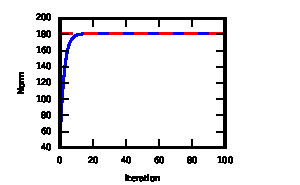
\includegraphics[width=\textwidth]{100IR4DTradPursnormplot}
	\caption{Average norm of the pursuer state cost with red dashed line as the average norm of the optimal value}
	\label{100IR4DTnp}
\end{subfigure}
\hfill
\begin{subfigure}[t]{0.475\textwidth}
	\centering
	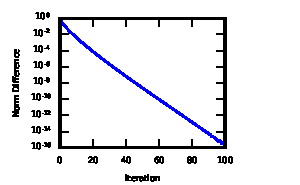
\includegraphics[width=\textwidth]{100IR4DTradPursdiffNormplot}
	\caption{Normalized difference in average norm between sequential pursuer state costs}
	\label{100IR4DTdnp}
\end{subfigure}
\caption{Diagnostic results of running 100 Iterations of Pursuit Value Iteration}
\label{100IR4DTdiag}
\end{figure} 
\begin{figure}
\centering
\begin{subfigure}[b]{0.475\textwidth}
	\centering
	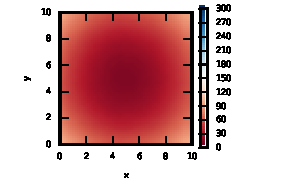
\includegraphics[width=\textwidth]{100IR4DTradPurspurscolorplot0}
	\caption{1 Iteration }
	\label{100IR4DTPCP0}
\end{subfigure}
\hfill
\begin{subfigure}[b]{0.475\textwidth}
	\centering
	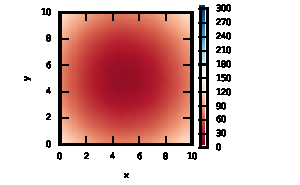
\includegraphics[width=\textwidth]{100IR4DTradPurspurscolorplot1}
	\caption{2 Iterations}
	\label{100IR4DTPCP1}
\end{subfigure}
\vskip\baselineskip
\begin{subfigure}[b]{0.475\textwidth}
	\centering
	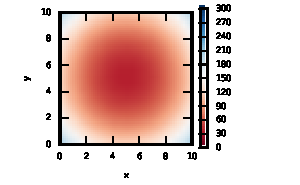
\includegraphics[width=\textwidth]{100IR4DTradPurspurscolorplot9}
	\caption{10 Iterations}
	\label{100IR4DTPCP9}
\end{subfigure}
\quad
\begin{subfigure}[b]{0.475\textwidth}
	\centering
	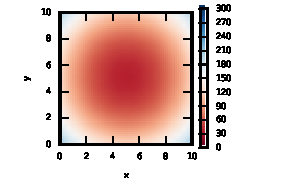
\includegraphics[width=\textwidth]{100IR4DTradPurspurscolorplot99}
	\caption{100 Iterations}
	\label{100IR4DTPCP99}
\end{subfigure}
\caption{State cost evolution when evader is at (5,5)}
\label{100IR4DTPCP}
\end{figure}

After the pursuer value iteration is run for a hundred iterations, the evader value iteration is also run for a hundred iterations with the updated pursuer cost, $J^{(100,1)}_p$. Just like with the pursuer value iteration, it took approximately an hour and a half to run one hundred iterations of evader value iteration, \Cref{4DVIrt}. The evolution of the evader state cost can be seen  in \Cref{100IR4DTECP}. Take note of the minimal difference in the state cost between ten and a hundred iterations. Notice that the average norm converges to the optimal average norm, \Cref{100IR4DTEnp}, and the difference between the average norm logarithmically decreases, \Cref{100IR4DTEdnp}. Notice that despite maximizing over the same cost function, the average norm converges to approximately the same value as in \Cref{100IR4DTnp}.
\begin{figure}[h!]
\centering
\begin{subfigure}[t]{0.475\textwidth}
	\centering
	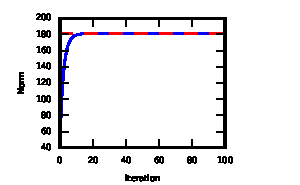
\includegraphics[width=\textwidth]{100IR4DTradEvadnormplot}
	\caption{Average norm of the evader state cost with red dashed line as the average norm of the optimal value}
	\label{100IR4DTEnp}
\end{subfigure}
\hfill
\begin{subfigure}[t]{0.475\textwidth}
	\centering
	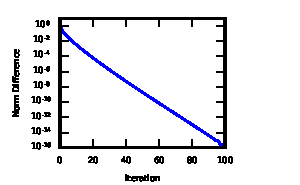
\includegraphics[width=\textwidth]{100IR4DTradEvaddiffNormplot}
	\caption{Normalized difference in average norm between sequential evader state costs}
	\label{100IR4DTEdnp}
\end{subfigure}
\caption{Diagnostic results of running 100 Iterations of Evader Value Iteration}
\label{100IR4DTEdiag}
\end{figure}  
\begin{figure}
\centering
\begin{subfigure}[b]{0.475\textwidth}
	\centering
	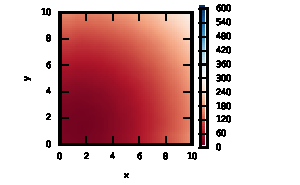
\includegraphics[width=\textwidth]{100IR4DTradEvadevadcolorplot0}
	\caption{1 Iteration }
	\label{100IR4DTECP0}
\end{subfigure}
\hfill
\begin{subfigure}[b]{0.475\textwidth}
	\centering
	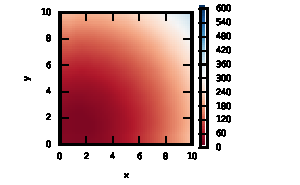
\includegraphics[width=\textwidth]{100IR4DTradEvadevadcolorplot1}
	\caption{2 Iterations}
	\label{100IR4DTECP1}
\end{subfigure}
\vskip\baselineskip
\begin{subfigure}[b]{0.475\textwidth}
	\centering
	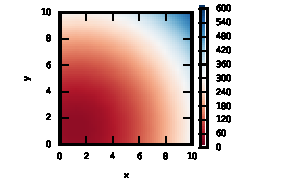
\includegraphics[width=\textwidth]{100IR4DTradEvadevadcolorplot9}
	\caption{10 Iterations}
	\label{100IR4DTECP9}
\end{subfigure}
\quad
\begin{subfigure}[b]{0.475\textwidth}
	\centering
	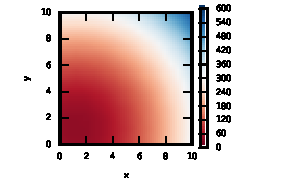
\includegraphics[width=\textwidth]{100IR4DTradEvadevadcolorplot99}
	\caption{100 Iterations}
	\label{100IR4DTECP99}
\end{subfigure}
\caption{State cost evolution when pursuer is at (1,1)}
\label{100IR4DTECP}
\end{figure}
\begin{table}
\caption{Value Iteration Program Run Times(sec)}
\label{4DVIrt}
\begin{center}
\begin{tabular}{||r|c|c||}\hline
  & 1 Iteration & 100 Iterations \\\hline
Pursuit & 57.6885 & 5942.2932 \\\hline
Evasion & 58.3154 & 5865.4880 \\\hline
\end{tabular}
\end{center}
\end{table}

Traditional value iteration was also implemented with \Cref{DPBRalg}. This algorithm was ran twice, once at $\Delta_{max} = 1E-2$ and $\delta_{max} = 1E-2$ for an equal comparison with the TVI algorithm  and once where $\Delta_{max} = 1E-5$ and $\delta_{max} = 1E-5$ to determine optimality to a point where changes in the state cost were no longer noticeable. For the $(\Delta_{max} = 1E-2,\delta_{max} = 1E-2)$ case, on the first best response run both the pursuer and evader state costs converge to an average norm of 179 in about 10 iterations as can be seen by the blue line in \Cref{BR4DTSPnp,BR4DTSEnp}. Changes to the control on this run are minor enough that there are no major changes in state costs on the second run as can be seen by the red line segment in the same figures. This causes the algorithm to end after only two runs. To run the entire algorithm it took almost twenty minutes, \Cref{BRPRun}. 
\begin{figure}[h!]
\centering
\begin{subfigure}[t]{0.475\textwidth}
	\centering
	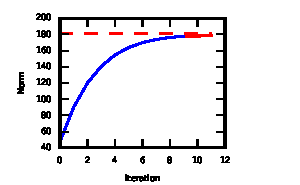
\includegraphics[width=\textwidth]{BR4DTSPursnormplot}
	\caption{Average norm of the pursuer state cost with red dashed line as the average norm of the optimal value}
	\label{BR4DTSPnp}
\end{subfigure}
\hfill
\begin{subfigure}[t]{0.475\textwidth}
	\centering
	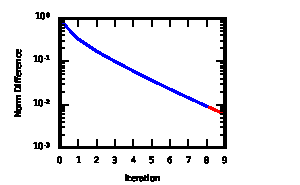
\includegraphics[width=\textwidth]{BR4DTSPursdiffNormplot}
	\caption{Normalized difference in average norm between sequential pursuer state costs}
	\label{BR4DTSPdnp}
\end{subfigure}
\caption{Pursuer diagnostic results of running Best Response Value Iteration Algorithm with $(\Delta_{max} = 1E-2,\delta_{max} = 1E-2)$. Blue solid line is the first run, while the red solid line is the second run}
\label{BR4DTSPdiag}
\end{figure}
\begin{figure}[h!]
\centering
\begin{subfigure}[t]{0.475\textwidth}
	\centering
	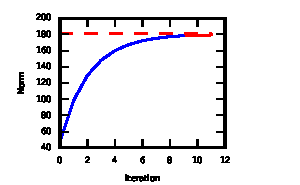
\includegraphics[width=\textwidth]{BR4DTSEvadnormplot}
	\caption{Average norm of the evader state cost with red dashed line as the average norm of the optimal value}
	\label{BR4DTSEnp}
\end{subfigure}
\hfill
\begin{subfigure}[t]{0.475\textwidth}
	\centering
	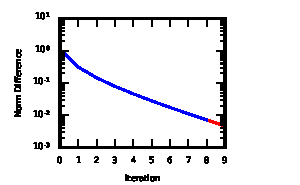
\includegraphics[width=\textwidth]{BR4DTSEvaddiffNormplot}
	\caption{Normalized difference in average norm between sequential evader state costs}
	\label{BR4DTSEdnp}
\end{subfigure}
\caption{Evader diagnostic results of running Best Response Value Iteration Algorithm with $(\Delta_{max} = 1E-2,\delta_{max} = 1E-2)$. Blue solid line is the first run, while the red solid line is the second run}
\label{BR4DTSEdiag}
\end{figure}

The pursuer state costs monotonically decrease toward the evaders position, \Cref{BR4DTSPcp}, while the evader's state costs monotonically decrease toward the pursuers position,\Cref{BR4DTSEcp}. The game was simulated with the pursuer starting at eight different positions and the evader starting at (5,5) as can be seen in \Cref{BR4DTSGp}. In each of these cases, the pursuer heads directly toward the evader while the evader heads in the opposite direct of the pursuer. Due to the pursuers faster speed in both the x and y axis, the distance between the pursuer and evader decreases directly to the origin, \Cref{BR4DTSGr}. It should be noted that due to the separation of the dynamics in the x and y axis, when the pursuer and evader have the same value on only one axis an oscillation occurs. This is due to the evader randomly darting to one or the other direction with the pursuer quickly following and overcoming the evader.
\begin{figure}[h!]
\centering
\begin{subfigure}[t]{0.475\textwidth}
	\centering
	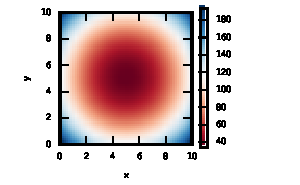
\includegraphics[width=\textwidth]{BR4DTSPurspurscolorplot}
	\caption{Pursuer state cost when evader is at (5,5)}
	\label{BR4DTSPcp}
\end{subfigure}
\hfill
\begin{subfigure}[t]{0.475\textwidth}
	\centering
	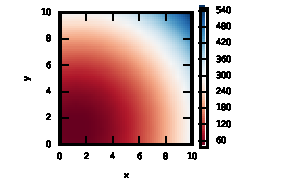
\includegraphics[width=\textwidth]{BR4DTSEvadevadcolorplot}
	\caption{Evader state cost when pursuer is at (1,1)}
	\label{BR4DTSEcp}
\end{subfigure}
\caption{State Costs after running Best Response Value Iteration Algorithm with $(\Delta_{max} = 1E-2,\delta_{max} = 1E-2)$}
\label{BR4DTScp}
\end{figure}
\begin{figure}
\centering
\begin{subfigure}[b]{0.3\textwidth}
	\centering
	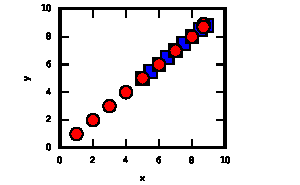
\includegraphics[width=\textwidth]{BR4DTSGamephaseplot1}
	\caption{(1,1) }
	\label{BR4DTSGp1}
\end{subfigure}
\hfill
\begin{subfigure}[b]{0.3\textwidth}
	\centering
	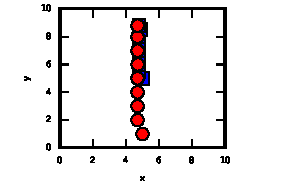
\includegraphics[width=\textwidth]{BR4DTSGamephaseplot2}
	\caption{(5,1)}
	\label{BR4DTSGp2}
\end{subfigure}
\hfill
\begin{subfigure}[b]{0.3\textwidth}
	\centering
	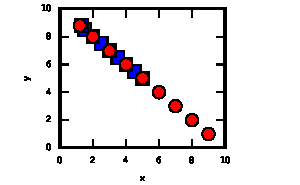
\includegraphics[width=\textwidth]{BR4DTSGamephaseplot3}
	\caption{(9,1)}
	\label{BR4DTSGp3}
\end{subfigure}
\vskip\baselineskip
\begin{subfigure}[b]{0.3\textwidth}
	\centering
	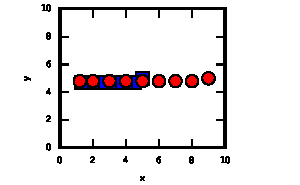
\includegraphics[width=\textwidth]{BR4DTSGamephaseplot4}
	\caption{(9,5) }
	\label{BR4DTSGp4}
\end{subfigure}
\hfill
\begin{subfigure}[b]{0.3\textwidth}
	\centering
	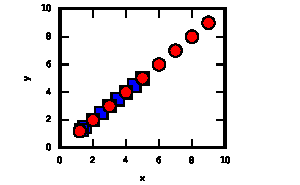
\includegraphics[width=\textwidth]{BR4DTSGamephaseplot5}
	\caption{(9,9)}
	\label{BR4DTSGp5}
\end{subfigure}
\hfill
\begin{subfigure}[b]{0.3\textwidth}
	\centering
	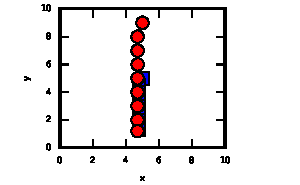
\includegraphics[width=\textwidth]{BR4DTSGamephaseplot6}
	\caption{(5,9)}
	\label{BR4DTSGp6}
\end{subfigure}
\vskip\baselineskip
\begin{subfigure}[b]{0.3\textwidth}
	\centering
	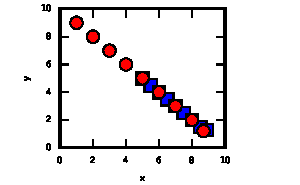
\includegraphics[width=\textwidth]{BR4DTSGamephaseplot7}
	\caption{(1,9) }
	\label{BR4DTSGp7}
\end{subfigure}
\quad
\begin{subfigure}[b]{0.3\textwidth}
	\centering
	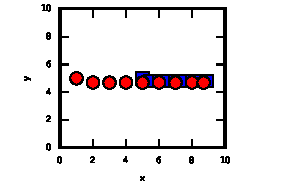
\includegraphics[width=\textwidth]{BR4DTSGamephaseplot8}
	\caption{(1,5)}
	\label{BR4DTSGp8}
\end{subfigure}
\caption{Pursuit-Evasion game with evader at (5,5) and pursuer at varying positions. 1 second intervals are used between each marker}
\label{BR4DTSGp}
\end{figure}
\begin{figure}
\centering
\begin{subfigure}[b]{0.3\textwidth}
	\centering
	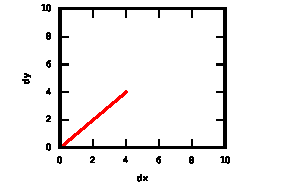
\includegraphics[width=\textwidth]{BR4DTSGamerelplot1}
	\caption{(1,1) }
	\label{BR4DTSGr1}
\end{subfigure}
\hfill
\begin{subfigure}[b]{0.3\textwidth}
	\centering
	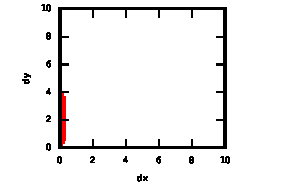
\includegraphics[width=\textwidth]{BR4DTSGamerelplot2}
	\caption{(5,1)}
	\label{BR4DTSGr2}
\end{subfigure}
\hfill
\begin{subfigure}[b]{0.3\textwidth}
	\centering
	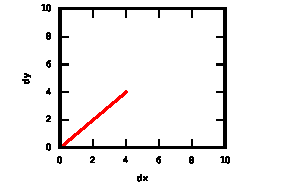
\includegraphics[width=\textwidth]{BR4DTSGamerelplot3}
	\caption{(9,1)}
	\label{BR4DTSGr3}
\end{subfigure}
\vskip\baselineskip
\begin{subfigure}[b]{0.3\textwidth}
	\centering
	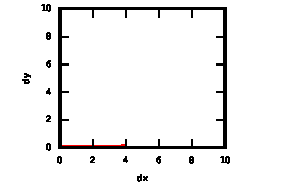
\includegraphics[width=\textwidth]{BR4DTSGamerelplot4}
	\caption{(9,5) }
	\label{BR4DTSGr4}
\end{subfigure}
\hfill
\begin{subfigure}[b]{0.3\textwidth}
	\centering
	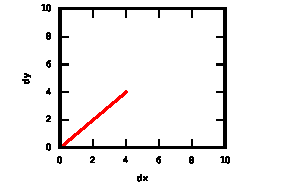
\includegraphics[width=\textwidth]{BR4DTSGamerelplot5}
	\caption{(9,9)}
	\label{BR4DTSGr5}
\end{subfigure}
\hfill
\begin{subfigure}[b]{0.3\textwidth}
	\centering
	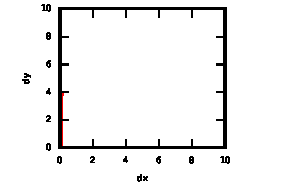
\includegraphics[width=\textwidth]{BR4DTSGamerelplot6}
	\caption{(5,9)}
	\label{BR4DTSGr6}
\end{subfigure}
\vskip\baselineskip
\begin{subfigure}[b]{0.3\textwidth}
	\centering
	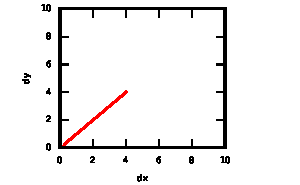
\includegraphics[width=\textwidth]{BR4DTSGamerelplot7}
	\caption{(1,9) }
	\label{BR4DTSGr7}
\end{subfigure}
\quad
\begin{subfigure}[b]{0.3\textwidth}
	\centering
	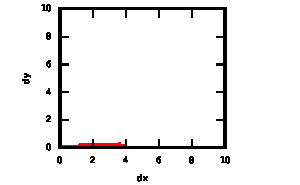
\includegraphics[width=\textwidth]{BR4DTSGamerelplot8}
	\caption{(1,5)}
	\label{BR4DTSGr8}
\end{subfigure}
\caption{Relative position of pursuer and evader in pursuit-Evasion game with evader at (5,5) and pursuer at varying positions}
\label{BR4DTSGr}
\end{figure}

A $(\Delta_{max} = 1E-5,\delta_{max} = 1E-5)$ case was also implemented to ensure that the $(\Delta_{max} = 1E-2,\delta_{max} = 1E-2)$ case ran to an appropriate termination. On the first best response run both the pursuer and evader state costs converge to an average norm of 180.97 in just over 25 iterations as seen by the blue solid line in \Cref{BR4DTCPnp,BR4DTCEnp}. The second run of best response again produces no notable change in the state cost of either the pursuer or the evader as seen by the red solid line in the same figures. Because of this the average norm of 180.97 will be considered optimal for the four-dimensional problem. In order to get this more accurate response, the algorithm ran for almost an hour, \Cref{BRPRun}. Despite the much longer run time, the results of the pursuit-evasion game do not noticeably change as can be seen by \Cref{BR4DTCcp,BR4DTCGp,BR4DTCGr} mirroring \Cref{BR4DTScp,BR4DTSGp,BR4DTSGr}. 
\begin{figure}[h!]
\centering
\begin{subfigure}[t]{0.475\textwidth}
	\centering
	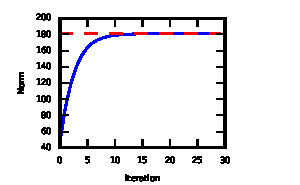
\includegraphics[width=\textwidth]{BR4DTCPursnormplot}
	\caption{Average norm of the pursuer state cost with red dashed line as the average norm of the optimal value}
	\label{BR4DTCPnp}
\end{subfigure}
\hfill
\begin{subfigure}[t]{0.475\textwidth}
	\centering
	\includegraphics[width=\textwidth]{BR4DTCPursdiffNormplot}
	\caption{Normalized difference in average norm between sequential pursuer state costs}
	\label{BR4DTCPdnp}
\end{subfigure}
\caption{Pursuer diagnostic results of running Best Response Value Iteration Algorithm with $(\Delta_{max} = 1E-5,\delta_{max} = 1E-5)$. Blue solid line is the first run, while the red solid line is the second run}
\label{BR4DTCPdiag}
\end{figure}
\begin{figure}[h!]
\centering
\begin{subfigure}[t]{0.475\textwidth}
	\centering
	\includegraphics[width=\textwidth]{BR4DTCEvadnormplot}
	\caption{Average norm of the evader state cost with red dashed line as the average norm of the optimal value}
	\label{BR4DTCEnp}
\end{subfigure}
\hfill
\begin{subfigure}[t]{0.475\textwidth}
	\centering
	\includegraphics[width=\textwidth]{BR4DTCEvaddiffNormplot}
	\caption{Normalized difference in average norm between sequential evader state costs}
	\label{BR4DTCEdnp}
\end{subfigure}
\caption{Evader diagnostic results of running Best Response Value Iteration Algorithm with $(\Delta_{max} = 1E-5,\delta_{max} = 1E-5)$. Blue solid line is the first run, while the red solid line is the second run}
\label{BR4DTCEdiag}
\end{figure}
\begin{figure}[h!]
\centering
\begin{subfigure}[t]{0.475\textwidth}
	\centering
	\includegraphics[width=\textwidth]{BR4DTCPurspurscolorplot}
	\caption{Pursuer state cost when evader is at (5,5)}
	\label{BR4DTCPcp}
\end{subfigure}
\hfill
\begin{subfigure}[t]{0.475\textwidth}
	\centering
	\includegraphics[width=\textwidth]{BR4DTCEvadevadcolorplot}
	\caption{Evader state cost when pursuer is at (1,1)}
	\label{BR4DTCEcp}
\end{subfigure}
\caption{State Costs after running Best Response Value Iteration Algorithm with $(\Delta_{max} = 1E-5,\delta_{max} = 1E-5)$}
\label{BR4DTCcp}
\end{figure}
\begin{figure}
\centering
\begin{subfigure}[b]{0.3\textwidth}
	\centering
	\includegraphics[width=\textwidth]{BR4DTCGamephaseplot1}
	\caption{(1,1) }
	\label{BR4DTCGp1}
\end{subfigure}
\hfill
\begin{subfigure}[b]{0.3\textwidth}
	\centering
	\includegraphics[width=\textwidth]{BR4DTCGamephaseplot2}
	\caption{(5,1)}
	\label{BR4DTCGp2}
\end{subfigure}
\hfill
\begin{subfigure}[b]{0.3\textwidth}
	\centering
	\includegraphics[width=\textwidth]{BR4DTCGamephaseplot3}
	\caption{(9,1)}
	\label{BR4DTCGp3}
\end{subfigure}
\vskip\baselineskip
\begin{subfigure}[b]{0.3\textwidth}
	\centering
	\includegraphics[width=\textwidth]{BR4DTCGamephaseplot4}
	\caption{(9,5) }
	\label{BR4DTCGp4}
\end{subfigure}
\hfill
\begin{subfigure}[b]{0.3\textwidth}
	\centering
	\includegraphics[width=\textwidth]{BR4DTCGamephaseplot5}
	\caption{(9,9)}
	\label{BR4DTCGp5}
\end{subfigure}
\hfill
\begin{subfigure}[b]{0.3\textwidth}
	\centering
	\includegraphics[width=\textwidth]{BR4DTCGamephaseplot6}
	\caption{(5,9)}
	\label{BR4DTCGp6}
\end{subfigure}
\vskip\baselineskip
\begin{subfigure}[b]{0.3\textwidth}
	\centering
	\includegraphics[width=\textwidth]{BR4DTCGamephaseplot7}
	\caption{(1,9) }
	\label{BR4DTCGp7}
\end{subfigure}
\quad
\begin{subfigure}[b]{0.3\textwidth}
	\centering
	\includegraphics[width=\textwidth]{BR4DTCGamephaseplot8}
	\caption{(1,5)}
	\label{BR4DTCGp8}
\end{subfigure}
\caption{Pursuit-Evasion game with evader at (5,5) and pursuer at varying positions. 1 second intervals are used between each marker}
\label{BR4DTCGp}
\end{figure}
\begin{figure}
\centering
\begin{subfigure}[b]{0.3\textwidth}
	\centering
	\includegraphics[width=\textwidth]{BR4DTCGamerelplot1}
	\caption{(1,1) }
	\label{BR4DTCGr1}
\end{subfigure}
\hfill
\begin{subfigure}[b]{0.3\textwidth}
	\centering
	\includegraphics[width=\textwidth]{BR4DTCGamerelplot2}
	\caption{(5,1)}
	\label{BR4DTCGr2}
\end{subfigure}
\hfill
\begin{subfigure}[b]{0.3\textwidth}
	\centering
	\includegraphics[width=\textwidth]{BR4DTCGamerelplot3}
	\caption{(9,1)}
	\label{BR4DTCGr3}
\end{subfigure}
\vskip\baselineskip
\begin{subfigure}[b]{0.3\textwidth}
	\centering
	\includegraphics[width=\textwidth]{BR4DTCGamerelplot4}
	\caption{(9,5) }
	\label{BR4DTCGr4}
\end{subfigure}
\hfill
\begin{subfigure}[b]{0.3\textwidth}
	\centering
	\includegraphics[width=\textwidth]{BR4DTCGamerelplot5}
	\caption{(9,9)}
	\label{BR4DTCGr5}
\end{subfigure}
\hfill
\begin{subfigure}[b]{0.3\textwidth}
	\centering
	\includegraphics[width=\textwidth]{BR4DTCGamerelplot6}
	\caption{(5,9)}
	\label{BR4DTCGr6}
\end{subfigure}
\vskip\baselineskip
\begin{subfigure}[b]{0.3\textwidth}
	\centering
	\includegraphics[width=\textwidth]{BR4DTCGamerelplot7}
	\caption{(1,9) }
	\label{BR4DTCGr7}
\end{subfigure}
\quad
\begin{subfigure}[b]{0.3\textwidth}
	\centering
	\includegraphics[width=\textwidth]{BR4DTCGamerelplot8}
	\caption{(1,5)}
	\label{BR4DTCGr8}
\end{subfigure}
\caption{Relative position of pursuer and evader in pursuit-Evasion game with evader at (5,5) and pursuer at varying positions}
\label{BR4DTCGr}
\end{figure}             

\subsection{Tensor-Based Value Iteration}
Tensor-Based Value Iteration can also be used to solve the pursuit-evasion game with simple Euclidean dynamics. Just as with traditional value iteration, before running \Cref{BRTVIalg} both the pursuer and evader TVI were run for 100 iterations to characterize the algorithm when run past completion. Once again both the pursuer and evader state cost were set to initialized such that $J^{(0,0)}_p(z_i) = (x_1-x_2)^2+(y_1-y_2)^2$ and $J^{(0,0)}_e(z_i) = (x_1-x_2)^2+(y_1-y_2)^2$. The pursuer TVI is run first for one hundred iterations. These one hundred iterations only take about eight minutes, \Cref{4DTTVIrt}. The evolution of the pursuer state cost can be seen  in \Cref{100IR4DTVIPCP}. Once again there is very little difference between the state cost at ten iterations and a hundred iterations. Notice that the average norm converges to the optimal average norm, \Cref{100IR4DTVInp}. The difference between the average norm logarithmically decreases until a difference of about $10^{-3}$ at which point the plot fluctuates about this point \Cref{100IR4DTVIdnp}. Average tensor rank remains constant at 3.60, \Cref{100IR4DTVIrkp}, while the fraction of states used fluctuates between about 0.020 and 0.013 of the original $21^4$ states, \Cref{100IR4DTVIsp}. 
\begin{figure}[h!]
\centering
\begin{subfigure}[t]{0.475\textwidth}
	\centering
	\includegraphics[width=\textwidth]{100IR4DTVIPursnormplot}
	\caption{Average norm of the pursuer state cost with red dashed line as the average norm of the optimal value}
	\label{100IR4DTVInp}
\end{subfigure}
\hfill
\begin{subfigure}[t]{0.475\textwidth}
	\centering
	\includegraphics[width=\textwidth]{100IR4DTVIPursdiffNormplot}
	\caption{Normalized difference in average norm between sequential pursuer state costs}
	\label{100IR4DTVIdnp}
\end{subfigure}
\vskip\baselineskip
\begin{subfigure}[t]{0.475\textwidth}
	\centering
	\includegraphics[width=\textwidth]{100IR4DTVIPursRankplot}
	\caption{Average rank of the pursuer state cost tensor}
	\label{100IR4DTVIrkp}
\end{subfigure}
\hfill
\begin{subfigure}[t]{0.475\textwidth}
	\centering
	\includegraphics[width=\textwidth]{100IR4DTVIPurssizeplot}
	\caption{Fraction of states used for the pursuer state cost tensor}
	\label{100IR4DTVIsp}
\end{subfigure}
\caption{Diagnostic results of running 100 Iterations of Pursuit TVI}
\label{100IR4DTVIdiag}
\end{figure} 
\begin{figure}
\centering
\begin{subfigure}[b]{0.475\textwidth}
	\centering
	\includegraphics[width=\textwidth]{100IR4DTVIPurspurscolorplot0}
	\caption{1 Iteration }
	\label{100IR4DTVIPCP0}
\end{subfigure}
\hfill
\begin{subfigure}[b]{0.475\textwidth}
	\centering
	\includegraphics[width=\textwidth]{100IR4DTVIPurspurscolorplot1}
	\caption{2 Iterations}
	\label{100IR4DTVIPCP1}
\end{subfigure}
\vskip\baselineskip
\begin{subfigure}[b]{0.475\textwidth}
	\centering
	\includegraphics[width=\textwidth]{100IR4DTVIPurspurscolorplot9}
	\caption{10 Iterations}
	\label{100IR4DTVIPCP9}
\end{subfigure}
\quad
\begin{subfigure}[b]{0.475\textwidth}
	\centering
	\includegraphics[width=\textwidth]{100IR4DTVIPurspurscolorplot99}
	\caption{100 Iterations}
	\label{100IR4DTVIPCP99}
\end{subfigure}
\caption{State cost evolution when evader is at (5,5)}
\label{100IR4DTVIPCP}
\end{figure}

After the pursuer TVI is run for a hundred iterations, the evader TVI is run for a hundred iterations with the updated pursuer cost, $J^{(100,1)}_p$. Just like the pursuer TVI, the evader TVI only takes about eight minutes to complete a hundred iterations, \Cref{4DTTVIrt}. The evolution of the evader state cost can be seen  in \Cref{100IR4DTVIECP}. The average norm still converges to the optimal average norm, \Cref{100IR4DTVIEnp}. Just as with pursuer TVI the difference between the average norm logarithmically decreases until a difference of about $10^{-3}$ at which point the plot fluctuates about this point \Cref{100IR4DTVIEdnp}. Average tensor rank also remains constant at 3.60, \Cref{100IR4DTVIErkp}, while the fraction of states used fluctuates between about 0.020 and 0.013 of the original $21^4$ states, \Cref{100IR4DTVIEsp}. Just as with traditional value iteration, the average norm converges to approximately the same value as in \Cref{100IR4DTVInp}.
\begin{figure}[h!]
\centering
\begin{subfigure}[t]{0.475\textwidth}
	\centering
	\includegraphics[width=\textwidth]{100IR4DTVIEvadnormplot}
	\caption{Average norm of the evader state cost with red dashed line as the average norm of the optimal value}
	\label{100IR4DTVIEnp}
\end{subfigure}
\hfill
\begin{subfigure}[t]{0.475\textwidth}
	\centering
	\includegraphics[width=\textwidth]{100IR4DTVIEvaddiffNormplot}
	\caption{Normalized difference in average norm between sequential evader state costs}
	\label{100IR4DTVIEdnp}
\end{subfigure}
\vskip\baselineskip
\begin{subfigure}[t]{0.475\textwidth}
	\centering
	\includegraphics[width=\textwidth]{100IR4DTVIEvadRankplot}
	\caption{Average rank of the evader state cost tensor}
	\label{100IR4DTVIErkp}
\end{subfigure}
\hfill
\begin{subfigure}[t]{0.475\textwidth}
	\centering
	\includegraphics[width=\textwidth]{100IR4DTVIEvadsizeplot}
	\caption{Fraction of states used for the evader state cost tensor}
	\label{100IR4DTVIEsp}
\end{subfigure}
\caption{Diagnostic results of running 100 Iterations of Evade TVI}
\label{100IR4DTVIEdiag}
\end{figure} 
\begin{figure}
\centering
\begin{subfigure}[b]{0.475\textwidth}
	\centering
	\includegraphics[width=\textwidth]{100IR4DTVIEvadevadcolorplot0}
	\caption{1 Iteration }
	\label{100IR4DTVIECP0}
\end{subfigure}
\hfill
\begin{subfigure}[b]{0.475\textwidth}
	\centering
	\includegraphics[width=\textwidth]{100IR4DTVIEvadevadcolorplot1}
	\caption{2 Iterations}
	\label{100IR4DTVIECP1}
\end{subfigure}
\vskip\baselineskip
\begin{subfigure}[b]{0.475\textwidth}
	\centering
	\includegraphics[width=\textwidth]{100IR4DTVIEvadevadcolorplot9}
	\caption{10 Iterations}
	\label{100IR4DTVIECP9}
\end{subfigure}
\quad
\begin{subfigure}[b]{0.475\textwidth}
	\centering
	\includegraphics[width=\textwidth]{100IR4DTVIEvadevadcolorplot99}
	\caption{100 Iterations}
	\label{100IR4DTVIECP99}
\end{subfigure}
\caption{State cost evolution when pursuer is at (1,1)}
\label{100IR4DTVIECP}
\end{figure}
\begin{table}
\caption{4D TVI Program Run Times(sec)}
\label{4DTTVIrt}
\begin{center}
\begin{tabular}{||r|c|c||}\hline
  & 1 Iteration & 100 Iterations \\\hline
Pursuit & 4.3525 & 473.1945 \\\hline
Evasion & 4.6160 & 483.1202 \\\hline
\end{tabular}
\end{center}
\end{table}

The four-dimensional problem was also solved using \Cref{BRTVIalg}. $\Delta_{max} = 1E-2$ and $\delta_{max} = 1E-2$ were used as the best response and the value iteration accuracy respectively. On the first best response run both the pursuer and evader state costs converge to an average norm of 179 in about 10 iterations as can be seen by the solid blue line in \Cref{BR4DTVIPnp,BR4DTVIEnp}. The average rank for both the pursuer and evader stays at 3.6 throughout, \Cref{BR4DTVIPrkp,BR4DTVIErkp}. In determining the new state costs, less than $1/50$ of the total states is used for each iteration of TVI, \Cref{BR4DTVIPsp,BR4DTVIEsp}. On the second run of best response, the changes remain minor resulting in virtually no change to the norm, rank, or states used for both the pursuer and the evader as can be seen by the solid red line in the previous figures, \Cref{BR4DTVIPdiag,BR4DTVIEdiag}. The entire Best Response TVI algorithm for the four-dimensional problem takes less than two minutes to complete, \Cref{BRPRun}. 
\begin{figure}[h!]
\centering
\begin{subfigure}[t]{0.475\textwidth}
	\centering
	\includegraphics[width=\textwidth]{BR4DTVIPursnormplot}
	\caption{Average norm of the pursuer state cost with red dashed line as the average norm of the optimal value}
	\label{BR4DTVIPnp}
\end{subfigure}
\hfill
\begin{subfigure}[t]{0.475\textwidth}
	\centering
	\includegraphics[width=\textwidth]{BR4DTVIPursdiffNormplot}
	\caption{Normalized difference in average norm between sequential pursuer state costs}
	\label{BR4DTVIPdnp}
\end{subfigure}
\vskip\baselineskip
\begin{subfigure}[t]{0.475\textwidth}
	\centering
	\includegraphics[width=\textwidth]{BR4DTVIPursRankplot}
	\caption{Average rank of the pursuer state cost tensor}
	\label{BR4DTVIPrkp}
\end{subfigure}
\hfill
\begin{subfigure}[t]{0.475\textwidth}
	\centering
	\includegraphics[width=\textwidth]{BR4DTVIPurssizeplot}
	\caption{Fraction of states used for the pursuer state cost tensor}
	\label{BR4DTVIPsp}
\end{subfigure}
\caption{Pursuer diagnostic results of running Best Response TVI Algorithm with $(\Delta_{max} = 1E-2,\delta_{max} = 1E-2)$. Blue solid line is the first run, while the red solid line is the second run}
\label{BR4DTVIPdiag}
\end{figure}
\begin{figure}[h!]
\centering
\begin{subfigure}[t]{0.475\textwidth}
	\centering
	\includegraphics[width=\textwidth]{BR4DTVIEvadnormplot}
	\caption{Average norm of the evader state cost with red dashed line as the average norm of the optimal value}
	\label{BR4DTVIEnp}
\end{subfigure}
\hfill
\begin{subfigure}[t]{0.475\textwidth}
	\centering
	\includegraphics[width=\textwidth]{BR4DTVIEvaddiffNormplot}
	\caption{Normalized difference in average norm between sequential evader state costs}
	\label{BR4DTVIEdnp}
\end{subfigure}
\vskip\baselineskip
\begin{subfigure}[t]{0.475\textwidth}
	\centering
	\includegraphics[width=\textwidth]{BR4DTVIEvadRankplot}
	\caption{Average rank of the evader state cost tensor}
	\label{BR4DTVIErkp}
\end{subfigure}
\hfill
\begin{subfigure}[t]{0.475\textwidth}
	\centering
	\includegraphics[width=\textwidth]{BR4DTVIEvadsizeplot}
	\caption{Fraction of states used for the evader state cost tensor}
	\label{BR4DTVIEsp}
\end{subfigure}
\caption{Evader diagnostic results of running Best Response TVI Algorithm with $(\Delta_{max} = 1E-2,\delta_{max} = 1E-2)$. Blue solid line is the first run, while the red solid line is the second run}
\label{BR4DTVIEdiag}
\end{figure}

The pursuer state costs monotonically decrease toward the evaders position, \Cref{BR4DTVIPcp}, while the evader's state costs monotonically decrease toward the pursuers position,\Cref{BR4DTVIEcp}. The pursuer heads directly towards the evader, while the evader heads in the opposite direction of the pursuer as can be seen in \Cref{BR4DTVIp}. Due to the pursuer's greater speed, the game has the pursuer constantly decreasing the distance between itself and the evader until capture as can be seen in \Cref{BR4DTVIr}.
\begin{figure}[h!]
\centering
\begin{subfigure}[t]{0.475\textwidth}
	\centering
	\includegraphics[width=\textwidth]{BR4DTVIPurspurscolorplot}
	\caption{Pursuer state cost when evader is at (5,5)}
	\label{BR4DTVIPcp}
\end{subfigure}
\hfill
\begin{subfigure}[t]{0.475\textwidth}
	\centering
	\includegraphics[width=\textwidth]{BR4DTVIEvadevadcolorplot}
	\caption{Evader state cost when pursuer is at (1,1)}
	\label{BR4DTVIEcp}
\end{subfigure}
\caption{State Costs after running Best Response TVI Algorithm with $(\Delta_{max} = 1E-2,\delta_{max} = 1E-2)$}
\label{BR4DTVIcp}
\end{figure}
\begin{figure}
\centering
\begin{subfigure}[b]{0.3\textwidth}
	\centering
	\includegraphics[width=\textwidth]{BR4DTVIphaseplot1}
	\caption{(1,1) }
	\label{BR4DTVIp1}
\end{subfigure}
\hfill
\begin{subfigure}[b]{0.3\textwidth}
	\centering
	\includegraphics[width=\textwidth]{BR4DTVIphaseplot2}
	\caption{(5,1)}
	\label{BR4DTVIp2}
\end{subfigure}
\hfill
\begin{subfigure}[b]{0.3\textwidth}
	\centering
	\includegraphics[width=\textwidth]{BR4DTVIphaseplot3}
	\caption{(9,1)}
	\label{BR4DTVIp3}
\end{subfigure}
\vskip\baselineskip
\begin{subfigure}[b]{0.3\textwidth}
	\centering
	\includegraphics[width=\textwidth]{BR4DTVIphaseplot4}
	\caption{(9,5) }
	\label{BR4DTVIp4}
\end{subfigure}
\hfill
\begin{subfigure}[b]{0.3\textwidth}
	\centering
	\includegraphics[width=\textwidth]{BR4DTVIphaseplot5}
	\caption{(9,9)}
	\label{BR4DTVIp5}
\end{subfigure}
\hfill
\begin{subfigure}[b]{0.3\textwidth}
	\centering
	\includegraphics[width=\textwidth]{BR4DTVIphaseplot6}
	\caption{(5,9)}
	\label{BR4DTVIp6}
\end{subfigure}
\vskip\baselineskip
\begin{subfigure}[b]{0.3\textwidth}
	\centering
	\includegraphics[width=\textwidth]{BR4DTVIphaseplot7}
	\caption{(1,9) }
	\label{BR4DTVIp7}
\end{subfigure}
\quad
\begin{subfigure}[b]{0.3\textwidth}
	\centering
	\includegraphics[width=\textwidth]{BR4DTVIphaseplot8}
	\caption{(1,5)}
	\label{BR4DTVIp8}
\end{subfigure}
\caption{Pursuit-Evasion game with evader at (5,5) and pursuer at varying positions. 1 second intervals are used between each marker}
\label{BR4DTVIp}
\end{figure}
\begin{figure}
\centering
\begin{subfigure}[b]{0.3\textwidth}
	\centering
	\includegraphics[width=\textwidth]{BR4DTVIrelplot1}
	\caption{(1,1) }
	\label{BR4DTVIr1}
\end{subfigure}
\hfill
\begin{subfigure}[b]{0.3\textwidth}
	\centering
	\includegraphics[width=\textwidth]{BR4DTVIrelplot2}
	\caption{(5,1)}
	\label{BR4DTVIr2}
\end{subfigure}
\hfill
\begin{subfigure}[b]{0.3\textwidth}
	\centering
	\includegraphics[width=\textwidth]{BR4DTVIrelplot3}
	\caption{(9,1)}
	\label{BR4DTVIr3}
\end{subfigure}
\vskip\baselineskip
\begin{subfigure}[b]{0.3\textwidth}
	\centering
	\includegraphics[width=\textwidth]{BR4DTVIrelplot4}
	\caption{(9,5) }
	\label{BR4DTVIr4}
\end{subfigure}
\hfill
\begin{subfigure}[b]{0.3\textwidth}
	\centering
	\includegraphics[width=\textwidth]{BR4DTVIrelplot5}
	\caption{(9,9)}
	\label{BR4DTVIr5}
\end{subfigure}
\hfill
\begin{subfigure}[b]{0.3\textwidth}
	\centering
	\includegraphics[width=\textwidth]{BR4DTVIrelplot6}
	\caption{(5,9)}
	\label{BR4DTVIr6}
\end{subfigure}
\vskip\baselineskip
\begin{subfigure}[b]{0.3\textwidth}
	\centering
	\includegraphics[width=\textwidth]{BR4DTVIrelplot7}
	\caption{(1,9) }
	\label{BR4DTVIr7}
\end{subfigure}
\quad
\begin{subfigure}[b]{0.3\textwidth}
	\centering
	\includegraphics[width=\textwidth]{BR4DTVIrelplot8}
	\caption{(1,5)}
	\label{BR4DTVIr8}
\end{subfigure}
\caption{Relative position of pursuer and evader in pursuit-Evasion game with evader at (5,5) and pursuer at varying positions}
\label{BR4DTVIr}
\end{figure}     

\subsection{Comparison of Traditional Value Iteration and TVI}
Both traditional value iteration and tensor-based value iteration can be used to solve the four-dimensional simple euclidean dynamics problem, however each method has its advantages and drawbacks. For the four-dimensional pursuit-evasion problem both traditional value iteration and TVI successfully solve the problem. This can be seen by the nearly identical solutions from all eight starting positions for both the state cost results from traditional value iteration and the state cost result from TVI as seen in \Cref{BR4DTSGp,BR4DTCGp,BR4DTVIp}. All average norms of the state costs also converge to the average norm of the optimal solution of 180.97, \Cref{BR4DTSPnp,BR4DTSEnp,BR4DTCPnp,BR4DTCEnp,BR4DTVIPnp,BR4DTVIEnp}. However, the precision of traditional value iteration can be more exact than TVI. This can be seen in the difference between \Cref{100IR4DTdnp,100IR4DTEdnp} and \Cref{100IR4DTVIdnp,100IR4DTVIEdnp}. While the traditional value iteration continues to become more precise until limited by the precision of the variable (about $10^{-16}$), TVI is constrained in its precision by the accuracy of the tensor approximation (for the given example about $10^{-3}$). Furthermore, TVI can only tighten its precision at the potential expense in increased run time. 

Although traditional value iteration has benefits when it comes to precision, TVI can compute the solution more efficiently. Using the $10^{-2}$ error bounds, TVI runs more than ten times faster than the traditional method as can be seen in \Cref{4DVIrt,4DTTVIrt,BRPRun}. Use of the TVI algorithm also conserves memory. As seen in \Cref{4Dstore}, the state cost representations of TVI are approximately an eighth the size of the four-dimensional arrays used to store the state costs in traditional value iteration. This four-dimensional example shows that TVI provides many benefits for problems already solvable by traditional value iteration.
\begin{table}
\caption{State Cost Storage}
\label{4Dstore}
\begin{center}
\begin{tabular}{||r|c|c||}\hline
  & Value Iteration & TTVI \\\hline
Pursuit & 8 MB & 883.3 kB \\\hline
Evasion & 8 MB & 1.1 MB \\\hline
\end{tabular}
\end{center}
\end{table}

\begin{table}
\caption{Best Response Program Run Times}
\label{BRPRun}
\begin{center}
\begin{tabular}{||r|c|c|c|c||}\hline
  & 4D Trad. VI(1E-2) & 4D Trad. VI(1E-5) & 4D TVI (1E-2) & 6D TVI (1E-2)\\\hline
Time (s) & 1152.3172 & 3123.4174 & 102.0020 & 593.2975 \\\hline

\end{tabular}
\end{center}
\end{table}  

\section{Six-Dimensional Problem}
For the six dimensional problem, the pursuer and evader adapt Dubins car dynamics as outlined in \cite{dubins}.  The pursuer and evader remain in a $10 \times 10$ two-dimensional  state space with the addition of a heading state for both. The six dimensions are the $x$ position of the pursuer $x_1$, the $y$ position of the pursuer $y_1$, the heading of the pursuer $\theta_1$, the $x$ position of the evader $x_2$, the $y$ position of the evader $y_2$, and the heading of the evader $\theta_2$. This results in a state space such that $z_i = (x_1,y_1,\theta_1,x_2,y_2,\theta_2)$. Each of the dimensions are bounded as follows:
\begin{eqnarray*}
x_1 & \in & [0,10]\\
y_1 & \in & [0,10]\\
\theta_1 & \in & [0,2\pi]\\
x_2 & \in & [0,10]\\
y_2 & \in & [0,10]\\
\theta_2 & \in & [0,2\pi].
\end{eqnarray*} 
Both the pursuer and the evader have a single control for their change in heading, respectively $u_1$ and $u_2$. These controls are bounded between $[-\dfrac{\pi}{4},\dfrac{\pi}{4}]$. The pursuer and evader each have a constant velocity as defined by $V_1$ and $V_2$ respectively. For this problem $V_1 = 1$ and $V_2 = 0.5$. This results in the following system dynamics:
\begin{eqnarray}\label{eqns2}
\dot{x}_1 & = & x_1 +V_1cos(\theta_1)dt,\\
\dot{y}_1 & = & y_1 +V_1sin(\theta_1)dt,\\
\dot{\theta_1}  & = & \theta_1 + V_1tan(u_1)dt\\
\dot{x}_2 & = & x_2 +V_2cos(\theta_2)dt,\\
\dot{y}_2 & = & y_2 +V_2sin(\theta_2)dt,\\
\dot{\theta_2}  & = & \theta_2 + V_2tan(u_2)dt.
\end{eqnarray}
Each dimension is again discretized into 21 equally spaced states for a total of $21^6 \approx 9\cdot10^7$ discrete states. This discretization creates the same discrete state space as for the four-dimensional problem for the $x$ and $y$ states. The theta values are discretized such that the four cardinal directions are included and $0$ and $2\pi$ are redundantly kept in the discretization as can be seen:
\begin{eqnarray*}
\theta_1 & \in & [0,\dfrac{\pi}{10},\dfrac{\pi}{5},\dfrac{3\pi}{10},\dfrac{2\pi}{5},\dfrac{\pi}{2},\dfrac{3\pi}{5},\dfrac{7\pi}{10},\dfrac{4\pi}{5},\dfrac{9\pi}{10},\pi,\dfrac{11\pi}{10},\dfrac{6\pi}{5},\dfrac{13\pi}{10},\dfrac{7\pi}{5},\dfrac{3\pi}{2},\dfrac{8\pi}{5},\dfrac{17\pi}{10},\dfrac{9\pi}{5},\dfrac{19\pi}{10},2\pi]\\
\theta_2 & \in & [0,\dfrac{\pi}{10},\dfrac{\pi}{5},\dfrac{3\pi}{10},\dfrac{2\pi}{5},\dfrac{\pi}{2},\dfrac{3\pi}{5},\dfrac{7\pi}{10},\dfrac{4\pi}{5},\dfrac{9\pi}{10},\pi,\dfrac{11\pi}{10},\dfrac{6\pi}{5},\dfrac{13\pi}{10},\dfrac{7\pi}{5},\dfrac{3\pi}{2},\dfrac{8\pi}{5},\dfrac{17\pi}{10},\dfrac{9\pi}{5},\dfrac{19\pi}{10},2\pi].
\end{eqnarray*} 
Value iteration can also be used to solve for the optimal cost at each state. The problem is modeled as in \Cref{peprobdes}. A state cost function based on the distance between the pursuer and evader was chosen: 
\begin{equation}\label{6cost}
G(z_i,u_1,u_2)= 10+(x_1-x_2)^2+(y_1-y_2)^2.
\end{equation}
The constant of $10$ is added to provided a buffer for the TVI approximation in order to prevent negative values. A discount factor of $\gamma = 0.7$ was chosen. Applying the state cost function and discount factor to \Cref{pbell} results in the update functions for the six-dimensional pursuit-evasion problem:
\begin{equation}\label{6pbell}
J_p^{(k+1,K)}(z_i)= \underset{u_1 }{\operatorname{min }}[10+(x_1-x_2)^2+(y_1-y_2)^2+0.7 J_p^{(k,K)}(z_j|z_i,u_1,u_2^K)],
\end{equation}
\begin{equation}\label{6ebell}
J_e^{(k+1,K)}(z_i)= \underset{u_2 }{\operatorname{max }}[10+(x_1-x_2)^2+(y_1-y_2)^2+0.7 J_e^{(k,K)}(z_j|z_i,u_1^K,u_2)].
\end{equation} 
By running \Cref{BRTVIalg} with \Cref{6pbell,6ebell} results in the given optimal value functions:
\begin{equation}\label{6pbropt}
J_p^{(*,*)}(z_i)= \underset{u_1 }{\operatorname{min }}[10+(x_1-x_2)^2+(y_1-y_2)^2+0.7 J_p^{(*,*)}(z_j|z_i,u_1,u_2^*)],
\end{equation}
\begin{equation}\label{6ebropt}
J_e^{(*,*)}(z_i)= \underset{u_2 }{\operatorname{max }}[10+(x_1-x_2)^2+(y_1-y_2)^2+0.7 J_e^{(*,*)}(z_j|z_i,u_1^*,u_2)].
\end{equation}    
These optimal value functions \ref{6pbropt} \ref{6ebropt} can be used to solve the following pursuit-evasion optimization problem:
\begin{eqnarray}\label{6opt}
&&\underset{u_1 }{\operatorname{min }}\underset{u_2 }{\operatorname{max }}[\int_{0}^{T}e^{-0.7t}(10+(x_1(t)-x_2(t))^2+(y_1(t)-y_2(t))^2)dt]\\
&\textnormal{s.t.}&\ref{eqns2}.
\end{eqnarray}

\subsection{Solving the Six-Dimensional Pursuit-Evasion Problem}
The excessive size of the six-dimensional pursuit-evasion game makes this problem hard to solve with traditional value iteration. One iteration of traditional VI on the pursuit problem takes over thirteen hours to complete. However, TVI may be used to solve the problem within some accuracy $\varepsilon$ in relatively short periods of time. Just as with the four-dimensional problem, before applying the best response TVI algorithm a hundred iterations of the pursuer and evader TVI were conducted on the six-dimensional problem. 

Once again both the pursuer and evader state cost were set to initialized such that $J^{(0,0)}_p(z_i) = (x_1-x_2)^2+(y_1-y_2)^2$ and $J^{(0,0)}_e(z_i) = (x_1-x_2)^2+(y_1-y_2)^2$. The pursuer TVI is run first for one hundred iterations. These hundred iterations only took about fifty minutes which is less than half the time it took traditional value iteration to run a hundred iterations of the four-dimensional pursuit problem, \Cref{6DTTVIrt}. The evolution of the pursuer state cost in relation to the x and y position of the pursuer can be seen  in \Cref{100IR6DTVIPCP}. Once again there is very little difference between the state cost at ten iterations and a hundred iterations. The average norm converges to a little over 180 as seen in \Cref{100IR6DTVInp}. The difference between the average norm logarithmically decreases until a difference of just over $10^{-3}$ at which point the plot fluctuates about this point \Cref{100IR6DTVIdnp}. Average tensor rank starts at 3.85 but quickly jumps up to just below 4.3, \Cref{100IR6DTVIrkp}. Fluctuating at about 0.0001 of the original $21^6$ states, the fraction of states used is even smaller than in the four-dimensional problem, \Cref{100IR6DTVIsp}.
\begin{figure}[h!]
\centering
\begin{subfigure}[t]{0.475\textwidth}
	\centering
	\includegraphics[width=\textwidth]{100IR6DTVIPursnormplot}
	\caption{Average norm of the pursuer state cost}
	\label{100IR6DTVInp}
\end{subfigure}
\hfill
\begin{subfigure}[t]{0.475\textwidth}
	\centering
	\includegraphics[width=\textwidth]{100IR6DTVIPursdiffNormplot}
	\caption{Normalized difference in average norm between sequential pursuer state costs}
	\label{100IR6DTVIdnp}
\end{subfigure}
\vskip\baselineskip
\begin{subfigure}[t]{0.475\textwidth}
	\centering
	\includegraphics[width=\textwidth]{100IR6DTVIPursRankplot}
	\caption{Average rank of the pursuer state cost tensor}
	\label{100IR6DTVIrkp}
\end{subfigure}
\hfill
\begin{subfigure}[t]{0.475\textwidth}
	\centering
	\includegraphics[width=\textwidth]{100IR6DTVIPurssizeplot}
	\caption{Fraction of states used for the pursuer state cost tensor}
	\label{100IR6DTVIsp}
\end{subfigure}
\caption{Diagnostic results of running 100 Iterations of Pursuit TVI}
\label{100IR6DTVIdiag}
\end{figure} 
\begin{figure}
\centering
\begin{subfigure}[b]{0.475\textwidth}
	\centering
	\includegraphics[width=\textwidth]{100IR6DTVIPurspurscolorplot0}
	\caption{1 Iteration }
	\label{100IR6DTVIPCP0}
\end{subfigure}
\hfill
\begin{subfigure}[b]{0.475\textwidth}
	\centering
	\includegraphics[width=\textwidth]{100IR6DTVIPurspurscolorplot1}
	\caption{2 Iterations}
	\label{100IR6DTVIPCP1}
\end{subfigure}
\vskip\baselineskip
\begin{subfigure}[b]{0.475\textwidth}
	\centering
	\includegraphics[width=\textwidth]{100IR6DTVIPurspurscolorplot9}
	\caption{10 Iterations}
	\label{100IR6DTVIPCP9}
\end{subfigure}
\quad
\begin{subfigure}[b]{0.475\textwidth}
	\centering
	\includegraphics[width=\textwidth]{100IR6DTVIPurspurscolorplot99}
	\caption{100 Iterations}
	\label{100IR6DTVIPCP99}
\end{subfigure}
\caption{State cost evolution with respect to pursuer x and y position when evader is at (5,5) and ($\theta_1 = 0,\theta_2=0$)}
\label{100IR6DTVIPCP}
\end{figure} 

After the pursuer TVI is run for a hundred iterations, the evader TVI is also run for a hundred iterations with the updated pursuer cost, $J^{(100,1)}_p$. Once again the evader TVI only takes about fifty minutes to complete a hundred iterations, \Cref{6DTTVIrt}. The evolution of the evader state cost in relation to the x and y position of the evader can be seen  in \Cref{100IR6DTVIECP}. Also of note is the evolution of the evader state cost in relation to the heading of both the pursuer and the evader as seen in \Cref{100IR6DTVITCP}. Notice how the state cost evolves from uniform in iteration one to having distinct minimum and maximum points in iteration 10. This pattern is especially impressive as the $\theta$-values do not have an inherent cost in \Cref{6cost}. The average norm of the evader, much like the pursuer, converges to just over 180 \Cref{100IR6DTVIEnp}. Just as with the pursuer, the difference between the average norm logarithmically decreases until a difference of just above $10^{-3}$ at which point the plot fluctuates about this point \Cref{100IR6DTVIEdnp}. Average tensor rank behaves the same as in the pursuer case by starting at about 3.85 and jumping to a point just below 4.3, \Cref{100IR6DTVIErkp}. The fraction of states used fluctuates again at about 0.0001 of the original $21^6$ states, \Cref{100IR6DTVIEsp}. Just as with the four-dimensional problem, the average norm converges to approximately the same value as in \Cref{100IR6DTVInp}.
\begin{figure}[h!]
\centering
\begin{subfigure}[t]{0.475\textwidth}
	\centering
	\includegraphics[width=\textwidth]{100IR6DTVIEvadnormplot}
	\caption{Average norm of the evader state cost}
	\label{100IR6DTVIEnp}
\end{subfigure}
\hfill
\begin{subfigure}[t]{0.475\textwidth}
	\centering
	\includegraphics[width=\textwidth]{100IR6DTVIEvaddiffNormplot}
	\caption{Normalized difference in average norm between sequential evader state costs}
	\label{100IR6DTVIEdnp}
\end{subfigure}
\vskip\baselineskip
\begin{subfigure}[t]{0.475\textwidth}
	\centering
	\includegraphics[width=\textwidth]{100IR6DTVIEvadRankplot}
	\caption{Average rank of the evader state cost tensor}
	\label{100IR6DTVIErkp}
\end{subfigure}
\hfill
\begin{subfigure}[t]{0.475\textwidth}
	\centering
	\includegraphics[width=\textwidth]{100IR6DTVIEvadsizeplot}
	\caption{Fraction of states used for the evader state cost tensor}
	\label{100IR6DTVIEsp}
\end{subfigure}
\caption{Diagnostic results of running 100 Iterations of Evade TVI}
\label{100IR6DTVIEdiag}
\end{figure} 
\begin{figure}
\centering
\begin{subfigure}[b]{0.475\textwidth}
	\centering
	\includegraphics[width=\textwidth]{100IR6DTVIEvadevadcolorplot0}
	\caption{1 Iteration }
	\label{100IR6DTVIECP0}
\end{subfigure}
\hfill
\begin{subfigure}[b]{0.475\textwidth}
	\centering
	\includegraphics[width=\textwidth]{100IR6DTVIEvadevadcolorplot1}
	\caption{2 Iterations}
	\label{100IR6DTVIECP1}
\end{subfigure}
\vskip\baselineskip
\begin{subfigure}[b]{0.475\textwidth}
	\centering
	\includegraphics[width=\textwidth]{100IR6DTVIEvadevadcolorplot9}
	\caption{10 Iterations}
	\label{100IR6DTVIECP9}
\end{subfigure}
\quad
\begin{subfigure}[b]{0.475\textwidth}
	\centering
	\includegraphics[width=\textwidth]{100IR6DTVIEvadevadcolorplot99}
	\caption{100 Iterations}
	\label{100IR6DTVIECP99}
\end{subfigure}
\caption{State cost evolution with respect to evader x and y position when pursuer is at (1,1) and ($\theta_1 = 0,\theta_2=0$)}
\label{100IR6DTVIECP}
\end{figure}
\begin{figure}
\centering
\begin{subfigure}[b]{0.475\textwidth}
	\centering
	\includegraphics[width=\textwidth]{100IR6DTVIEvadthetacolorplot0}
	\caption{1 Iteration }
	\label{100IR6DTVITCP0}
\end{subfigure}
\hfill
\begin{subfigure}[b]{0.475\textwidth}
	\centering
	\includegraphics[width=\textwidth]{100IR6DTVIEvadthetacolorplot1}
	\caption{2 Iterations}
	\label{100IR6DTVITCP1}
\end{subfigure}
\vskip\baselineskip
\begin{subfigure}[b]{0.475\textwidth}
	\centering
	\includegraphics[width=\textwidth]{100IR6DTVIEvadthetacolorplot9}
	\caption{10 Iterations}
	\label{100IR6DTVITCP9}
\end{subfigure}
\quad
\begin{subfigure}[b]{0.475\textwidth}
	\centering
	\includegraphics[width=\textwidth]{100IR6DTVIEvadthetacolorplot99}
	\caption{100 Iterations}
	\label{100IR6DTVITCP99}
\end{subfigure}
\caption{State cost evolution with respect to heading when pursuer is at (1,1) and the evader is at (9,9)}
\label{100IR6DTVITCP}
\end{figure}
\begin{table}
\caption{6D TVI Program Run Times(sec)}
\label{6DTTVIrt}
\begin{center}
\begin{tabular}{||r|c|c||}\hline
  & 1 Iteration & 100 Iterations \\\hline
Pursuit & 22.7885 & 2883.9859 \\\hline
Evasion & 22.6637 & 2838.0722 \\\hline
\end{tabular}
\end{center}
\end{table}

Using \Cref{BRTVIalg}, the six-dimensional pursuit-evasion problem was solved. Just as with the four-dimensional problem, $\Delta_{max} = 1E-2$ and $\delta_{max} = 1E-2$ were used as the best response and the value iteration accuracy respectively. On the first best response run both the pursuer and evader state costs converge to an average norm of about 180 in about ten iterations as can be seen by the blue line in \Cref{BR6DTVIPnp,BR6DTVIEnp}. For both the pursuer and the evader, the average rank starts at 3.85 and quickly climbs to just below 4.30 before leveling off, \Cref{BR6DTVIPrkp,BR6DTVIErkp}. Generally only about $1/10000$ of the total states are used for each iteration of TVI, \Cref{BR6DTVIPrkp,BR6DTVIErkp}. On the second run of best response, the changes remain minor resulting in virtually no change to the norm, rank, or states used for both the pursuer and the evader as can be seen by the red line in \Cref{BR6DTVIPdiag,BR6DTVIEdiag}. The entire algorithm takes just under ten minutes to complete, \Cref{BRPRun}. This is about half the time that the traditional value iteration took for the four-dimensional problem and a much shorter time than the thirteen plus hours that a single iteration of traditional value iteration takes for the six-dimensional problem.
\begin{figure}[h!]
\centering
\begin{subfigure}[t]{0.475\textwidth}
	\centering
	\includegraphics[width=\textwidth]{BR6DTVIPursnormplot}
	\caption{Average norm of the pursuer state cost with red dashed line as the average norm of the optimal value}
	\label{BR6DTVIPnp}
\end{subfigure}
\hfill
\begin{subfigure}[t]{0.475\textwidth}
	\centering
	\includegraphics[width=\textwidth]{BR6DTVIPursdiffNormplot}
	\caption{Normalized difference in average norm between sequential pursuer state costs}
	\label{BR6DTVIPdnp}
\end{subfigure}
\vskip\baselineskip
\begin{subfigure}[t]{0.475\textwidth}
	\centering
	\includegraphics[width=\textwidth]{BR6DTVIPursRankplot}
	\caption{Average rank of the pursuer state cost tensor}
	\label{BR6DTVIPrkp}
\end{subfigure}
\hfill
\begin{subfigure}[t]{0.475\textwidth}
	\centering
	\includegraphics[width=\textwidth]{BR6DTVIPurssizeplot}
	\caption{Fraction of states used for the pursuer state cost tensor}
	\label{BR6DTVIPsp}
\end{subfigure}
\caption{Pursuer diagnostic results of running Best Response TVI Algorithm with $(\Delta_{max} = 1E-2,\delta_{max} = 1E-2)$. Blue solid line is the first run, while the red solid line is the second run}
\label{BR6DTVIPdiag}
\end{figure}
\begin{figure}[h!]
\centering
\begin{subfigure}[t]{0.475\textwidth}
	\centering
	\includegraphics[width=\textwidth]{BR6DTVIEvadnormplot}
	\caption{Average norm of the evader state cost with red dashed line as the average norm of the optimal value}
	\label{BR6DTVIEnp}
\end{subfigure}
\hfill
\begin{subfigure}[t]{0.475\textwidth}
	\centering
	\includegraphics[width=\textwidth]{BR6DTVIEvaddiffNormplot}
	\caption{Normalized difference in average norm between sequential evader state costs}
	\label{BR6DTVIEdnp}
\end{subfigure}
\vskip\baselineskip
\begin{subfigure}[t]{0.475\textwidth}
	\centering
	\includegraphics[width=\textwidth]{BR6DTVIEvadRankplot}
	\caption{Average rank of the evader state cost tensor}
	\label{BR6DTVIErkp}
\end{subfigure}
\hfill
\begin{subfigure}[t]{0.475\textwidth}
	\centering
	\includegraphics[width=\textwidth]{BR6DTVIEvadsizeplot}
	\caption{Fraction of states used for the evader state cost tensor}
	\label{BR6DTVIEsp}
\end{subfigure}
\caption{Evader diagnostic results of running Best Response TVI Algorithm with $(\Delta_{max} = 1E-2,\delta_{max} = 1E-2)$. Blue solid line is the first run, while the red solid line is the second run}
\label{BR6DTVIEdiag}
\end{figure}

Just as in the four-dimensional problem, the pursuer state costs monotonically decrease toward the evaders position, \Cref{BR6DTVIPcp}, while the evader's state costs monotonically decrease toward the pursuers position,\Cref{BR6DTVIEcp}. The state costs follow a similar pattern with regard to the heading of the pursuer and the evader. It can be seen in \Cref{BR6DTVITcp} that the state cost monotonically decreases when the pursuer or evader heading is toward the other player. 
\begin{figure}[h!]
\centering
\begin{subfigure}[t]{0.3\textwidth}
	\centering
	\includegraphics[width=\textwidth]{BR6DTVIPurspurscolorplot}
	\caption{Pursuer state cost in respect to the pursuer's x and y position when evader is at (5,5) and ($\theta_1 = 0,\theta_2=0$)}
	\label{BR6DTVIPcp}
\end{subfigure}
\hfill
\begin{subfigure}[t]{0.3\textwidth}
	\centering
	\includegraphics[width=\textwidth]{BR6DTVIEvadevadcolorplot}
	\caption{Evader state cost in respect to the evader's x and y position when pursuer is at (1,1) and ($\theta_1 = 0,\theta_2=0$)}
	\label{BR6DTVIEcp}
\end{subfigure}
\hfill
\begin{subfigure}[t]{0.3\textwidth}
	\centering
	\includegraphics[width=\textwidth]{BR6DTVIEvadthetacolorplot1}
	\caption{Evader state cost with respect to $\theta_1$ and $\theta_2$ when pursuer is at (1,1) and the evader is at (9,9)}
	\label{BR6DTVITcp}
\end{subfigure}
\caption{State Costs after running Best Response TVI Algorithm with $(\Delta_{max} = 1E-2,\delta_{max} = 1E-2)$}
\label{BR6DTVIcp}
\end{figure}

Using the optimal state costs $J_p^{(*,*)}$ and $J_e^{(*,*)}$ , two different problems are solved. The first is a standard problem where the pursuer starting at (1,1) and with a head $\theta_1 = 0$ chases an evader starting at (5,5) with a heading of $\theta_2 = 0$. The pursuer and evader both adjust their headings to the optimal solution of approximately $\pi/4$. Due to the pursuer's greater speed, the game has the pursuer constantly decreasing the distance between itself and the evader until capture as can be seen in \Cref{6DSG,6DS}.
\begin{figure}
\centering
\begin{subfigure}[b]{0.3\textwidth}
	\centering
	\includegraphics[width=\textwidth]{6DSGmovieplot0}
	\caption{0 s.}
	\label{6DSG0}
\end{subfigure}
\hfill
\begin{subfigure}[b]{0.3\textwidth}
	\centering
	\includegraphics[width=\textwidth]{6DSGmovieplot1}
	\caption{1 s.}
	\label{6DSG1}
\end{subfigure}
\hfill
\begin{subfigure}[b]{0.3\textwidth}
	\centering
	\includegraphics[width=\textwidth]{6DSGmovieplot2}
	\caption{2 s.}
	\label{6DSG2}
\end{subfigure}
\vskip\baselineskip
\begin{subfigure}[b]{0.3\textwidth}
	\centering
	\includegraphics[width=\textwidth]{6DSGmovieplot3}
	\caption{3 s.}
	\label{6DSG3}
\end{subfigure}
\hfill
\begin{subfigure}[b]{0.3\textwidth}
	\centering
	\includegraphics[width=\textwidth]{6DSGmovieplot4}
	\caption{4 s.}
	\label{6DSG4}
\end{subfigure}
\hfill
\begin{subfigure}[b]{0.3\textwidth}
	\centering
	\includegraphics[width=\textwidth]{6DSGmovieplot5}
	\caption{5 s.}
	\label{6DSG5}
\end{subfigure}
\vskip\baselineskip
\begin{subfigure}[b]{0.3\textwidth}
	\centering
	\includegraphics[width=\textwidth]{6DSGmovieplot6}
	\caption{6 s.}
	\label{6DSG6}
\end{subfigure}
\hfill
\begin{subfigure}[b]{0.3\textwidth}
	\centering
	\includegraphics[width=\textwidth]{6DSGmovieplot7}
	\caption{7 s.}
	\label{6DSG7}
\end{subfigure}
\hfill
\begin{subfigure}[b]{0.3\textwidth}
	\centering
	\includegraphics[width=\textwidth]{6DSGmovieplot8}
	\caption{8 s.}
	\label{6DSG8}
\end{subfigure}
\vskip\baselineskip
\begin{subfigure}[b]{0.3\textwidth}
	\centering
	\includegraphics[width=\textwidth]{6DSGmovieplot9}
	\caption{9 s.}
	\label{6DSG9}
\end{subfigure}
\hfill
\begin{subfigure}[b]{0.3\textwidth}
	\centering
	\includegraphics[width=\textwidth]{6DSGmovieplot10}
	\caption{10 s.}
	\label{6DSG10}
\end{subfigure}
\hfill
\begin{subfigure}[b]{0.3\textwidth}
	\centering
	\includegraphics[width=\textwidth]{6DSGmovieplot11}
	\caption{11 s.}
	\label{6DSG11}
\end{subfigure}
\caption{Pursuit-Evasion Game with Pursuer starting at (1,1) with $\theta_1 =0$ heading and Evader starting at (5,5) with $\theta_2 =0$ heading}
\label{6DSG}
\end{figure}
\begin{figure}[h!]
\centering
\begin{subfigure}[t]{0.475\textwidth}
	\centering
	\includegraphics[width=\textwidth]{6DSGphaseplot}
	\caption{Position of Pursuer and Evader with one second intervals and heading}
	\label{6DSGp}
\end{subfigure}
\hfill
\begin{subfigure}[t]{0.475\textwidth}
	\centering
	\includegraphics[width=\textwidth]{6DSGrelplot}
	\caption{Relative distance between pursuer and evader}
	\label{6DSGr}
\end{subfigure}
\caption{Pursuit-Evasion Game with Pursuer starting at (1,1) with $\theta_1 =0$ heading and Evader starting at (5,5) with $\theta_2 =0$ heading}
\label{6DS}
\end{figure}

The second problem involves the pursuer starting at (7,5) with a heading of $\theta_1 = 0$ and the evader behind the pursuer at (5,5) and a heading of $\theta_2 = 0$. In this game the pursuer has to make a wide sweep around in order to get on the tail of the evader while the evader dodges below the pursuer,\Cref{6DAG,6DAGp}. In this case the pursuer actually has to increase the distance between itself and the evader before it can close the distance as seen in \Cref{6DAGr}. This is a counter intuitive movement for the pursuer when examining the value function \Cref{6pbell}. This shows that best response TVI can solve non-intuitive problems.
\begin{figure}
\centering
\begin{subfigure}[b]{0.3\textwidth}
	\centering
	\includegraphics[width=\textwidth]{6DAGmovieplot0}
	\caption{0 s.}
	\label{6DAG0}
\end{subfigure}
\hfill
\begin{subfigure}[b]{0.3\textwidth}
	\centering
	\includegraphics[width=\textwidth]{6DAGmovieplot1}
	\caption{1 s.}
	\label{6DAG1}
\end{subfigure}
\hfill
\begin{subfigure}[b]{0.3\textwidth}
	\centering
	\includegraphics[width=\textwidth]{6DAGmovieplot2}
	\caption{2 s.}
	\label{6DAG2}
\end{subfigure}
\vskip\baselineskip
\begin{subfigure}[b]{0.3\textwidth}
	\centering
	\includegraphics[width=\textwidth]{6DAGmovieplot3}
	\caption{3 s.}
	\label{6DAG3}
\end{subfigure}
\hfill
\begin{subfigure}[b]{0.3\textwidth}
	\centering
	\includegraphics[width=\textwidth]{6DAGmovieplot4}
	\caption{4 s.}
	\label{6DAG4}
\end{subfigure}
\hfill
\begin{subfigure}[b]{0.3\textwidth}
	\centering
	\includegraphics[width=\textwidth]{6DAGmovieplot5}
	\caption{5 s.}
	\label{6DAG5}
\end{subfigure}
\vskip\baselineskip
\begin{subfigure}[b]{0.3\textwidth}
	\centering
	\includegraphics[width=\textwidth]{6DAGmovieplot6}
	\caption{6 s.}
	\label{6DAG6}
\end{subfigure}
\hfill
\begin{subfigure}[b]{0.3\textwidth}
	\centering
	\includegraphics[width=\textwidth]{6DAGmovieplot7}
	\caption{7 s.}
	\label{6DAG7}
\end{subfigure}
\hfill
\begin{subfigure}[b]{0.3\textwidth}
	\centering
	\includegraphics[width=\textwidth]{6DAGmovieplot8}
	\caption{8 s.}
	\label{6DAG8}
\end{subfigure}
\vskip\baselineskip
\begin{subfigure}[b]{0.3\textwidth}
	\centering
	\includegraphics[width=\textwidth]{6DAGmovieplot9}
	\caption{9 s.}
	\label{6DAG9}
\end{subfigure}
\hfill
\begin{subfigure}[b]{0.3\textwidth}
	\centering
	\includegraphics[width=\textwidth]{6DAGmovieplot10}
	\caption{10 s.}
	\label{6DAG10}
\end{subfigure}
\hfill
\begin{subfigure}[b]{0.3\textwidth}
	\centering
	\includegraphics[width=\textwidth]{6DAGmovieplot11}
	\caption{11 s.}
	\label{6DAG11}
\end{subfigure}
\caption{Pursuit-Evasion Game with Pursuer starting at (7,5) with $\theta_1 =0$ heading and Evader starting at (5,5) with $\theta_2 =0$ heading}
\label{6DAG}
\end{figure}
\begin{figure}[h!]
\centering
\begin{subfigure}[t]{0.475\textwidth}
	\centering
	\includegraphics[width=\textwidth]{6DAGphaseplot}
	\caption{Position of Pursuer and Evader with one second intervals and heading}
	\label{6DAGp}
\end{subfigure}
\hfill
\begin{subfigure}[t]{0.475\textwidth}
	\centering
	\includegraphics[width=\textwidth]{6DAGrelplot}
	\caption{Relative distance between pursuer and evader}
	\label{6DAGr}
\end{subfigure}
\caption{Pursuit-Evasion Game with Pursuer starting at (7,5) with $\theta_1 =0$ heading and Evader starting at (5,5) with $\theta_2 =0$ heading}
\label{6DA}
\end{figure} 
%% This is an example first chapter.  You should put chapter/appendix that you
%% write into a separate file, and add a line \include{yourfilename} to
%% main.tex, where `yourfilename.tex' is the name of the chapter/appendix file.
%% You can process specific files by typing their names in at the 
%% \files=
%% prompt when you run the file main.tex through LaTeX.
\chapter{Conclusion}\label{chp:con}
Best Response TVI and the underlying TVI algorithm have a number of advantages and disadvantages. This chapter will begin by exploring both the advantages and disadvantages of TVI as they relate to solving pursuit-evasion problems. A reflection on the constraints imposed by TVI's disadvantages will also be included in the first section. After detailing the benefits and constraints of TVI, a number of potential improvements for future research will be suggested. Finally, last remarks will be given on the importance of the research presented in this paper.  

\section{Summary of Results}
Tensor-based value iteration's ability to compute a solution in an efficient manner is the method's single greatest benefit. This method reduces the computational time of a four-dimensional problem to approximately a tenth of the time and makes a six-dimensional problem efficiently computable. However, TVI and the Best Response TVI algorithm still have a variety of problems. First, as stated in \Cref{chp:examples}, TVI only provides an approximation which can be held to some accuracy $\epsilon$. While $\epsilon$ can be reduced to some very small value, doing so can reduce the benefits of TVI by resulting in approximate tensors with large tensor ranks. As noted in \Cref{chp:TT}, the larger the ranks become the computational complexity of using tensor-trains increases dramatically. For this reason, using TVI often resulted in a balancing act of accuracy and complexity. Because of this, using TVI often required manually determining an accuracy that would maintain low-rank.

Maintaining low-rank often created restrictions on the modeling of a problem. Creating large capture regions or other discontinuity producing areas often strained TVI in finding a low-rank approximation. This was especially troublesome considering that the approximations often took the largest toll when the pursuer and evader were in close distance of each other. These restrictions required a relatively simple game in which the pursuer tried to minimize the distance between itself and the evader while the evader attempted to maximize this value.

The approximate nature of TVI also created a problem with potentially negative values. Often when the state cost for a particular state was either zero or close to zero, TVI would approximate this to a negative value. These values could potentially spiral out of control making the entirety of the state space converge to $-\infty$ as the number of iterations approached $\infty$. For this reason a constant of 10 was added to the state cost in \Cref{4cost,6cost}.

Despite a variety of shortcomings, Best Response TVI makes numerous problems efficiently solvable as detailed in \Cref{chp:examples}. As noted for the six-dimensional problem, using TVI reduces the time required to find a solution from weeks for traditional value iteration to less than half an hour. For some problems, such as the four-dimensional problem in \Cref{chp:examples}, the results for Best Response TVI and traditional value iteration are indistinguishable with Best Response TVI taking only a tenth of the time.           

\section{Future Directions}
The Best Response TVI algorithm provides a great basis for improvement. As already noted, best response TVI requires manual input of three different accuracy values, one for the tensor, value iteration, and best response. An algorithm capable of adjusting each of these accuracies to ensure the most accurate solution possible without causing either the rank to become too large or for the algorithm to enter a never ending loop would greatly assist in the usability of the algorithm. This modified algorithm could self-adjust to determine the optimal accuracy of the problem without requiring prior research or guess work to determine sufficient accuracies.

Numerous potential methods could be used to increase the accuracy of the solution by combining best response TVI with other methods. One such method could be to use the TVI approximation to create a full state array and continue the algorithm with traditional value iteration. Another method could be to use TVI to approximate the majority of the state space while using traditional value iteration to determine small areas of the state space that either require more precise accuracy or are not naturally low rank such as absorption regions.

Finally there are numerous ways to test best response TVI with a more complex state space or dynamics. This paper has constrained its use of best response TVI to vehicles navigating a two-dimensional space such as with cars. There is potential that best response can be used to navigate three-dimensional space such as with aircraft that can have variable altitude. More complex dynamics could include adding the effects of friction or wind resistance. Applying best response TVI to an environment with obstacles would also require overcoming a variety of complications due to discontinuities in the state space. These are just a few of the many future opportunities to conduct research with best response TVI.    


\section{Final Remarks}
Best Response TVI builds on the work of a variety of methods in order to efficiently solve pursuit-evasion games. The computational efficiency of best response TVI enables platforms with limited computational power to solve complex problems in an efficient manner. This is especially true for autonomous vehicles in pursuit-evasion environments. For example, suppose best response TVI was ran overnight to produce controls for an autonomous spy vehicle to tail a certain target using a vehicle that has Dubins dynamics with a certain maximum speed and turning radius. However, halfway through the mission the target decides to change vehicles to one with a different maximum speed or turning radius. Best response TVI would allow the autonomous spy vehicle to quickly approximate new optimal controls and continue with the mission. Best response TVI holds the potential to solve problems that would take days in hours and problems that would take hours in minutes.       

%\appendix
%\chapter{Tables}

\begin{table}
\caption{Value Iteration Program Run Times(sec)}
\label{4dVIrt}
\begin{center}
\begin{tabular}{||r|c|c||}\hline
  & 1 Iteration & 100 Iterations \\\hline
Pursuit & 57.6885 & 5942.2932 \\\hline
Evasion & 58.3154 & 5865.4880 \\\hline
\end{tabular}
\end{center}
\end{table}

\begin{table}
\caption{TVI Program Run Times(sec)}
\label{4dTTVIrt}
\begin{center}
\begin{tabular}{||r|c|c||}\hline
  & 1 Iteration & 100 Iterations \\\hline
Pursuit & 4.3525 & 473.1945 \\\hline
Evasion & 4.6160 & 483.1202 \\\hline
\end{tabular}
\end{center}
\end{table}

\begin{table}
\caption{State Cost Storage}
\label{4dstore}
\begin{center}
\begin{tabular}{||r|c|c||}\hline
  & Value Iteration & TTVI \\\hline
Pursuit & 8 MB & 883.3 kB \\\hline
Evasion & 8 MB & 1.1 MB \\\hline
\end{tabular}
\end{center}
\end{table}

\begin{table}
\caption{Best Response Program Run Times}
\label{BRRun}
\begin{center}
\begin{tabular}{||r|c|c|c|c||}\hline
  & 4D Traditional VI(1E-2) & 4D Traditional VI(1E-5) & 4D TVI (1E-2) & 6D TVI (1E-2)\\\hline
Time (s) & 1152.3172 & 3123.4174 & 102.0020 & 593.2975 \\\hline

\end{tabular}
\end{center}
\end{table}

\clearpage
\newpage

%\chapter{Figures}

\vspace*{-3in}

\begin{figure}
\vspace{2.4in}
\centering
\includegraphics[scale=1]{bvpregions}
\caption{A state space divided into capture,escape, and regions of play \cite{bardi2}}
\label{bvpregions}
\end{figure}
\clearpage
\newpage

\begin{figure}
\vspace{2.4in}
\centering
\begin{subfigure}[b]{0.475\textwidth}
	\centering
	\includegraphics[width=\textwidth]{bvpresult1}
	\caption{Approximate value function when $v_1 = 1$, $v_2 = 1$}
	\label{bvpresult1}
\end{subfigure}
\hfill
\begin{subfigure}[b]{0.475\textwidth}
	\centering
	\includegraphics[width=\textwidth]{bvpresult2}
	\caption{Approximate value function when $v_1 = 5$, $v_2 = 1$}
	\label{bvpresult2}
\end{subfigure}
\caption{Results for one-dimensional pursuit-evasion games \cite{bardi2}}
\label{bvpresults}
\end{figure}
\clearpage
\newpage

\begin{figure}
\vspace{2.4in}
\centering
\begin{subfigure}[b]{0.475\textwidth}
	\centering
	\includegraphics[width=\textwidth]{rrt500}
	\caption{Pursuit-Evasion $\textnormal{RRT}^*$ run for 500 iterations }
	\label{rrt500}
\end{subfigure}
\hfill
\begin{subfigure}[b]{0.475\textwidth}
	\centering
	\includegraphics[width=\textwidth]{rrt3000}
	\caption{Pursuit-Evasion $\textnormal{RRT}^*$ run for 3000 iterations}
	\label{rrt3000}
\end{subfigure}
\vskip\baselineskip
\begin{subfigure}[b]{0.475\textwidth}
	\centering
	\includegraphics[width=\textwidth]{rrt5000}
	\caption{Pursuit-Evasion $\textnormal{RRT}^*$ run for 5000 iterations}
	\label{rrt5000}
\end{subfigure}
\quad
\begin{subfigure}[b]{0.475\textwidth}
	\centering
	\includegraphics[width=\textwidth]{rrt10000}
	\caption{Pursuit-Evasion $\textnormal{RRT}^*$ run for 10000 iterations}
	\label{rrt10000}
\end{subfigure}
\caption{Pursuit-Evasion $\textnormal{RRT}^*$ \cite{karaman}}
\label{rrtfig}
\end{figure}
\clearpage
\newpage

\begin{figure}
\vspace{2.4in}
\centering
\begin{subfigure}[b]{0.475\textwidth}
	\centering
	\includegraphics[width=\textwidth]{rrtobs500}
	\caption{Pursuit-Evasion $\textnormal{RRT}^*$ run for 500 iterations}
	\label{rrtobs500}
\end{subfigure}
\hfill
\begin{subfigure}[b]{0.475\textwidth}
	\centering
	\includegraphics[width=\textwidth]{rrtobs3000}
	\caption{Pursuit-Evasion $\textnormal{RRT}^*$ run for 3000 iterations}
	\label{rrtobs3000}
\end{subfigure}
\vskip\baselineskip
\begin{subfigure}[b]{0.475\textwidth}
	\centering
	\includegraphics[width=\textwidth]{rrtobs5000}
	\caption{Pursuit-Evasion $\textnormal{RRT}^*$ run for 5000 iterations}
	\label{rrtobs5000}
\end{subfigure}
\quad
\begin{subfigure}[b]{0.475\textwidth}
	\centering
	\includegraphics[width=\textwidth]{rrtobs10000}
	\caption{Pursuit-Evasion $\textnormal{RRT}^*$ run for 10000 iterations}
	\label{rrtobs10000}
\end{subfigure}
\caption{Pursuit-Evasion $\textnormal{RRT}^*$ in a field with obstacles\cite{karaman}}
\label{rrtobsfig}
\end{figure}
\clearpage
\newpage

\begin{figure}
\vspace{2.4in}
\centering
\begin{subfigure}[b]{0.475\textwidth}
	\centering
	\includegraphics[width=\textwidth]{rrtdubins}
	\caption{Pursuit-Evasion $\textnormal{RRT}^*$ run for 3000 iterations}
	\label{rrtdubins}
\end{subfigure}
\hfill
\begin{subfigure}[b]{0.475\textwidth}
	\centering
	\includegraphics[width=\textwidth]{rrtobsdubins}
	\caption{Pursuit-Evasion $\textnormal{RRT}^*$ run for 3000 iterations in a field with obstacles}
	\label{rrtobsdubins}
\end{subfigure}
\caption{Pursuit-Evasion $\textnormal{RRT}^*$ on a problem with Dubins dynamics \cite{karaman}}
\label{rrtdubinsfig}
\end{figure}
\clearpage
\newpage

\begin{figure}
\vspace{2.4in}
\centering
\includegraphics[scale=1]{gorodglide}
\caption{Optimal glide path with vertical and horizontal velocities \cite{gorod}}
\label{gorodglide}
\end{figure}
\clearpage
\newpage

\begin{figure}
\vspace{2.4in}
\centering
\includegraphics[scale=1]{gorodstates}
\caption{Fraction of states evaluated by TTVI in optimal glide problem \cite{gorod}}
\label{gorodstates}
\end{figure}
\clearpage
\newpage

\begin{figure}
\vspace{2.4in}
\centering
\includegraphics[scale=3]{VIpursplot1}
\caption{Pursuer at (1,1) captures stationary evader at (5,5) after the first Pursuit Value Iteration Run}
\label{VIpursplot1}
\end{figure}
\clearpage
\newpage

\begin{figure}
\vspace{2.4in}
\centering
\includegraphics[scale=3]{VIpursplot2}
\caption{Pursuer at (5,1) captures stationary evader at (5,5) after the first Pursuit Value Iteration Run}
\label{VIpursplot2}
\end{figure}
\clearpage
\newpage

\begin{figure}
\vspace{2.4in}
\centering
\includegraphics[scale=3]{VIpursplot3}
\caption{Pursuer at (9,1) captures stationary evader at (5,5) after the first Pursuit Value Iteration Run}
\label{VIpursplot3}
\end{figure}
\clearpage
\newpage

\begin{figure}
\vspace{2.4in}
\centering
\includegraphics[scale=3]{VIpursplot4}
\caption{Pursuer at (9,5) captures stationary evader at (5,5) after the first Pursuit Value Iteration Run}
\label{VIpursplot4}
\end{figure}
\clearpage
\newpage

\begin{figure}
\vspace{2.4in}
\centering
\includegraphics[scale=3]{VIpursplot5}
\caption{Pursuer at (9,9) captures stationary evader at (5,5) after the first Pursuit Value Iteration Run}
\label{VIpursplot5}
\end{figure}
\clearpage
\newpage

\begin{figure}
\vspace{2.4in}
\centering
\includegraphics[scale=3]{VIpursplot6}
\caption{Pursuer at (5,9) captures stationary evader at (5,5) after the first Pursuit Value Iteration Run}
\label{VIpursplot6}
\end{figure}
\clearpage
\newpage

\begin{figure}
\vspace{2.4in}
\centering
\includegraphics[scale=3]{VIpursplot7}
\caption{Pursuer at (1,9) captures stationary evader at (5,5) after the first Pursuit Value Iteration Run}
\label{VIpursplot7}
\end{figure}
\clearpage
\newpage

\begin{figure}
\vspace{2.4in}
\centering
\includegraphics[scale=3]{VIpursplot8}
\caption{Pursuer at (1,5) captures stationary evader at (5,5) after the first Pursuit Value Iteration Run}
\label{VIpursplot8}
\end{figure}
\clearpage
\newpage

\begin{figure}
\vspace{2.4in}
\centering
\includegraphics[scale=0.25]{VIpursue0}
\caption{State Cost of the Pursuer when the Evader is at (5,5) after one iteration}
\label{VIpursue0}
\end{figure}
\clearpage
\newpage

\begin{figure}
\vspace{2.4in}
\centering
\includegraphics[scale=0.25]{VIpursue10}
\caption{State Cost of the Pursuer when the Evader is at (5,5) after eleven iterations}
\label{VIpursue10}
\end{figure}
\clearpage
\newpage

\begin{figure}
\vspace{2.4in}
\centering
\includegraphics[scale=0.25]{VIpursue98}
\caption{State Cost of the Pursuer when the Evader is at (5,5) after ninety-nine iterations}
\label{VIpursue98}
\end{figure}
\clearpage
\newpage

\begin{figure}
\vspace{2.4in}
\centering
\includegraphics[scale=0.25]{VIpursue99}
\caption{State Cost of the Pursuer when the Evader is at (5,5) after a hundred iterations}
\label{VIpursue99}
\end{figure}
\clearpage
\newpage

\begin{figure}
\vspace{2.4in}
\centering
\includegraphics[scale=3]{VIevadplot1}
\caption{Evader at (5,5) evades stationary pursuer at (1,1) after the first Evade Value Iteration Run}
\label{VIevadplot1}
\end{figure}
\clearpage
\newpage

\begin{figure}
\vspace{2.4in}
\centering
\includegraphics[scale=3]{VIevadplot2}
\caption{Evader at (5,5) evades stationary pursuer at (5,1) after the first Evade Value Iteration Run}
\label{VIevadplot2}
\end{figure}
\clearpage
\newpage

\begin{figure}
\vspace{2.4in}
\centering
\includegraphics[scale=3]{VIevadplot3}
\caption{Evader at (5,5) evades stationary pursuer at (9,1) after the first Evade Value Iteration Run}
\label{VIevadplot3}
\end{figure}
\clearpage
\newpage

\begin{figure}
\vspace{2.4in}
\centering
\includegraphics[scale=3]{VIevadplot4}
\caption{Evader at (5,5) evades stationary pursuer at (9,5) after the first Evade Value Iteration Run}
\label{VIevadplot4}
\end{figure}
\clearpage
\newpage

\begin{figure}
\vspace{2.4in}
\centering
\includegraphics[scale=3]{VIevadplot5}
\caption{Evader at (5,5) evades stationary pursuer at (9,9) after the first Evade Value Iteration Run}
\label{VIevadplot5}
\end{figure}
\clearpage
\newpage

\begin{figure}
\vspace{2.4in}
\centering
\includegraphics[scale=3]{VIevadplot6}
\caption{Evader at (5,5) evades stationary pursuer at (5,9) after the first Evade Value Iteration Run}
\label{VIevadplot6}
\end{figure}
\clearpage
\newpage

\begin{figure}
\vspace{2.4in}
\centering
\includegraphics[scale=3]{VIevadplot7}
\caption{Evader at (5,5) evades stationary pursuer at (1,9) after the first Evade Value Iteration Run}
\label{VIevadplot7}
\end{figure}
\clearpage
\newpage

\begin{figure}
\vspace{2.4in}
\centering
\includegraphics[scale=3]{VIevadplot8}
\caption{Evader at (5,5) evades stationary pursuer at (1,5) after the first Evade Value Iteration Run}
\label{VIevadplot8}
\end{figure}
\clearpage
\newpage

\begin{figure}
\vspace{2.4in}
\centering
\includegraphics[scale=0.25]{VIevade0}
\caption{State Cost of the Evader when the Pursuer is at (1,1) after one iteration}
\label{VIevade0}
\end{figure}
\clearpage
\newpage

\begin{figure}
\vspace{2.4in}
\centering
\includegraphics[scale=0.25]{VIevade10}
\caption{State Cost of the Evader when the Pursuer is at (1,1) after elven iterations}
\label{VIevade10}
\end{figure}
\clearpage
\newpage

\begin{figure}
\vspace{2.4in}
\centering
\includegraphics[scale=0.25]{VIevade98}
\caption{State Cost of the Evader when the Pursuer is at (1,1) after ninety-nine iterations}
\label{VIevade98}
\end{figure}
\clearpage
\newpage

\begin{figure}
\vspace{2.4in}
\centering
\includegraphics[scale=0.25]{VIevade99}
\caption{State Cost of the Evader when the Pursuer is at (1,1) after a hundred iterations}
\label{VIevade99}
\end{figure}
\clearpage
\newpage

\begin{figure}
\vspace{2.4in}
\centering
\includegraphics[scale=3]{VIpursbr1plot1}
\caption{Pursuer at (1,1) captures evader at (5,5) after the second Pursuit Value Iteration Run}
\label{VIpursbr1plot1}
\end{figure}
\clearpage
\newpage

\begin{figure}
\vspace{2.4in}
\centering
\includegraphics[scale=3]{VIpursbr1plot2}
\caption{Pursuer at (5,1) captures evader at (5,5) after the second Pursuit Value Iteration Run}
\label{VIpursbr1plot2}
\end{figure}
\clearpage
\newpage

\begin{figure}
\vspace{2.4in}
\centering
\includegraphics[scale=3]{VIpursbr1plot3}
\caption{Pursuer at (9,1) captures evader at (5,5) after the second Pursuit Value Iteration Run}
\label{VIpursbr1plot3}
\end{figure}
\clearpage
\newpage

\begin{figure}
\vspace{2.4in}
\centering
\includegraphics[scale=3]{VIpursbr1plot4}
\caption{Pursuer at (9,5) captures evader at (5,5) after the second Pursuit Value Iteration Run}
\label{VIpursbr1plot4}
\end{figure}
\clearpage
\newpage

\begin{figure}
\vspace{2.4in}
\centering
\includegraphics[scale=3]{VIpursbr1plot5}
\caption{Pursuer at (9,9) captures evader at (5,5) after the second Pursuit Value Iteration Run}
\label{VIpursbr1plot5}
\end{figure}
\clearpage
\newpage

\begin{figure}
\vspace{2.4in}
\centering
\includegraphics[scale=3]{VIpursbr1plot6}
\caption{Pursuer at (5,9) captures evader at (5,5) after the second Pursuit Value Iteration Run}
\label{VIpursbr1plot6}
\end{figure}
\clearpage
\newpage

\begin{figure}
\vspace{2.4in}
\centering
\includegraphics[scale=3]{VIpursbr1plot7}
\caption{Pursuer at (1,9) captures evader at (5,5) after the second Pursuit Value Iteration Run}
\label{VIpursbr1plot7}
\end{figure}
\clearpage
\newpage

\begin{figure}
\vspace{2.4in}
\centering
\includegraphics[scale=3]{VIpursbr1plot8}
\caption{Pursuer at (1,5) captures evader at (5,5) after the second Pursuit Value Iteration Run}
\label{VIpursbr1plot8}
\end{figure}
\clearpage
\newpage

\begin{figure}
\vspace{2.4in}
\centering
\includegraphics[scale=0.25]{VIpursue1br0}
\caption{State Cost of the Pursuer when the Evader is at (5,5) after one iteration}
\label{VIpursue1br0}
\end{figure}
\clearpage
\newpage

\begin{figure}
\vspace{2.4in}
\centering
\includegraphics[scale=0.25]{VIpursue1br10}
\caption{State Cost of the Pursuer when the Evader is at (5,5) after eleven iterations}
\label{VIpursue1br10}
\end{figure}
\clearpage
\newpage

\begin{figure}
\vspace{2.4in}
\centering
\includegraphics[scale=0.25]{VIpursue1br98}
\caption{State Cost of the Pursuer when the Evader is at (5,5) after ninety-nine iterations}
\label{VIpursue1br98}
\end{figure}
\clearpage
\newpage

\begin{figure}
\vspace{2.4in}
\centering
\includegraphics[scale=0.25]{VIpursue1br99}
\caption{State Cost of the Pursuer when the Evader is at (5,5) after a hundred iterations}
\label{VIpursue1br99}
\end{figure}
\clearpage
\newpage

\begin{figure}
\vspace{2.4in}
\centering
\includegraphics[scale=3]{VIevadbrplot1}
\caption{Pursuer at (1,1) captures evader at (5,5) after the second Evade Value Iteration Run}
\label{VIevadbrplot1}
\end{figure}
\clearpage
\newpage

\begin{figure}
\vspace{2.4in}
\centering
\includegraphics[scale=3]{VIevadbrplot2}
\caption{Pursuer at (5,1) captures evader at (5,5) after the second Evade Value Iteration Run}
\label{VIevadbrplot2}
\end{figure}
\clearpage
\newpage

\begin{figure}
\vspace{2.4in}
\centering
\includegraphics[scale=3]{VIevadbrplot3}
\caption{Pursuer at (9,1) captures evader at (5,5) after the second Evade Value Iteration Run}
\label{VIevadbrplot3}
\end{figure}
\clearpage
\newpage

\begin{figure}
\vspace{2.4in}
\centering
\includegraphics[scale=3]{VIevadbrplot4}
\caption{Pursuer at (9,5) captures evader at (5,5) after the second Evade Value Iteration Run}
\label{VIevadbrplot4}
\end{figure}
\clearpage
\newpage

\begin{figure}
\vspace{2.4in}
\centering
\includegraphics[scale=3]{VIevadbrplot5}
\caption{Pursuer at (9,9) captures evader at (5,5) after the second Evade Value Iteration Run}
\label{VIevadbrplot5}
\end{figure}
\clearpage
\newpage

\begin{figure}
\vspace{2.4in}
\centering
\includegraphics[scale=3]{VIevadbrplot6}
\caption{Pursuer at (5,9) captures evader at (5,5) after the second Evade Value Iteration Run}
\label{VIevadbrplot6}
\end{figure}
\clearpage
\newpage

\begin{figure}
\vspace{2.4in}
\centering
\includegraphics[scale=3]{VIevadbrplot7}
\caption{Pursuer at (1,9) captures evader at (5,5) after the second Evade Value Iteration Run}
\label{VIevadbrplot7}
\end{figure}
\clearpage
\newpage

\begin{figure}
\vspace{2.4in}
\centering
\includegraphics[scale=3]{VIevadbrplot8}
\caption{Pursuer at (1,5) captures evader at (5,5) after the second Evade Value Iteration Run}
\label{VIevadbrplot8}
\end{figure}
\clearpage
\newpage

\begin{figure}
\vspace{2.4in}
\centering
\includegraphics[scale=0.25]{VIevadebr0}
\caption{State Cost of the Evader when the Pursuer is at (1,1) after one iteration}
\label{VIevadebr0}
\end{figure}
\clearpage
\newpage

\begin{figure}
\vspace{2.4in}
\centering
\includegraphics[scale=0.25]{VIevadebr10}
\caption{State Cost of the Evader when the Pursuer is at (1,1) after elven iterations}
\label{VIevadebr10}
\end{figure}
\clearpage
\newpage

\begin{figure}
\vspace{2.4in}
\centering
\includegraphics[scale=0.25]{VIevadebr98}
\caption{State Cost of the Evader when the Pursuer is at (1,1) after ninety-nine iterations}
\label{VIevadebr98}
\end{figure}
\clearpage
\newpage

\begin{figure}
\vspace{2.4in}
\centering
\includegraphics[scale=0.25]{VIevadebr99}
\caption{State Cost of the Evader when the Pursuer is at (1,1) after a hundred iterations}
\label{VIevadebr99}
\end{figure}
\clearpage
\newpage

\begin{figure}
\vspace{2.4in}
\centering
\includegraphics[scale=3]{VIpursbr2plot1}
\caption{Pursuer at (1,1) captures evader at (5,5) after the third Pursuit Value Iteration Run}
\label{VIpursbr2plot1}
\end{figure}
\clearpage
\newpage

\begin{figure}
\vspace{2.4in}
\centering
\includegraphics[scale=3]{VIpursbr2plot2}
\caption{Pursuer at (5,1) captures evader at (5,5) after the third Pursuit Value Iteration Run}
\label{VIpursbr2plot2}
\end{figure}
\clearpage
\newpage

\begin{figure}
\vspace{2.4in}
\centering
\includegraphics[scale=3]{VIpursbr2plot3}
\caption{Pursuer at (9,1) captures evader at (5,5) after the third Pursuit Value Iteration Run}
\label{VIpursbr2plot3}
\end{figure}
\clearpage
\newpage

\begin{figure}
\vspace{2.4in}
\centering
\includegraphics[scale=3]{VIpursbr2plot4}
\caption{Pursuer at (9,5) captures evader at (5,5) after the third Pursuit Value Iteration Run}
\label{VIpursbr2plot4}
\end{figure}
\clearpage
\newpage

\begin{figure}
\vspace{2.4in}
\centering
\includegraphics[scale=3]{VIpursbr2plot5}
\caption{Pursuer at (9,9) captures evader at (5,5) after the third Pursuit Value Iteration Run}
\label{VIpursbr2plot5}
\end{figure}
\clearpage
\newpage

\begin{figure}
\vspace{2.4in}
\centering
\includegraphics[scale=3]{VIpursbr2plot6}
\caption{Pursuer at (5,9) captures evader at (5,5) after the third Pursuit Value Iteration Run}
\label{VIpursbr2plot6}
\end{figure}
\clearpage
\newpage

\begin{figure}
\vspace{2.4in}
\centering
\includegraphics[scale=3]{VIpursbr2plot7}
\caption{Pursuer at (1,9) captures evader at (5,5) after the third Pursuit Value Iteration Run}
\label{VIpursbr2plot7}
\end{figure}
\clearpage
\newpage

\begin{figure}
\vspace{2.4in}
\centering
\includegraphics[scale=3]{VIpursbr2plot8}
\caption{Pursuer at (1,5) captures evader at (5,5) after the third Pursuit Value Iteration Run}
\label{VIpursbr2plot8}
\end{figure}
\clearpage
\newpage

\begin{figure}
\vspace{2.4in}
\centering
\includegraphics[scale=0.25]{VIpursue2br0}
\caption{State Cost of the Pursuer when the Evader is at (5,5) after one iteration}
\label{VIpursue2br0}
\end{figure}
\clearpage
\newpage

\begin{figure}
\vspace{2.4in}
\centering
\includegraphics[scale=0.25]{VIpursue2br99}
\caption{State Cost of the Pursuer when the Evader is at (5,5) after a hundred iterations}
\label{VIpursue2br99}
\end{figure}
\clearpage
\newpage

\begin{figure}
\vspace{2.4in}
\centering
\includegraphics[scale=3]{4DTradPurs0diffNormplot}
\caption{Change in Norm of Pursuer State Value for each iteration of traditional VI}
\label{4DTradPurs0diffNormplot}
\end{figure}
\clearpage
\newpage

\begin{figure}
\vspace{2.4in}
\centering
\includegraphics[scale=3]{4DTradPurs0normplot}
\caption{Norm of Pursuer State Value for each iteration of traditional VI}
\label{4DTradPurs0normplot}
\end{figure}
\clearpage
\newpage

\begin{figure}
\vspace{2.4in}
\centering
\includegraphics[scale=3]{4DTradEvad0diffNormplot}
\caption{Change in Norm of Evader State Value for each iteration of traditional VI}
\label{4DTradEvad0diffNormplot}
\end{figure}
\clearpage
\newpage

\begin{figure}
\vspace{2.4in}
\centering
\includegraphics[scale=3]{4DTradEvad0normplot}
\caption{Norm of Evader State Value for each iteration of traditional VI}
\label{4DTradEvad0normplot}
\end{figure}
\clearpage
\newpage

\begin{figure}
\vspace{2.4in}
\centering
\includegraphics[scale=3]{4DTradPurs1diffNormplot}
\caption{Change in Norm of Pursuer State Value for each iteration of traditional VI}
\label{4DTradPurs1diffNormplot}
\end{figure}
\clearpage
\newpage

\begin{figure}
\vspace{2.4in}
\centering
\includegraphics[scale=3]{4DTradPurs1normplot}
\caption{Norm of Pursuer State Value for each iteration of traditional VI}
\label{4DTradPurs1normplot}
\end{figure}
\clearpage
\newpage

\begin{figure}
\vspace{2.4in}
\centering
\includegraphics[scale=3]{4DTradPurspurscolorplot}
\caption{Pursuer State Value when Evader is at (5,5)}
\label{4DTradPurspurscolorplot}
\end{figure}
\clearpage
\newpage

\begin{figure}
\vspace{2.4in}
\centering
\includegraphics[scale=3]{4DTradEvad1diffNormplot}
\caption{Change in Norm of Evader State Value for each iteration of traditional VI}
\label{4DTradEvad1diffNormplot}
\end{figure}
\clearpage
\newpage

\begin{figure}
\vspace{2.4in}
\centering
\includegraphics[scale=3]{4DTradEvad1normplot}
\caption{Norm of Evader State Value for each iteration of traditional VI}
\label{4DTradEvad1normplot}
\end{figure}
\clearpage
\newpage

\begin{figure}
\vspace{2.4in}
\centering
\includegraphics[scale=3]{4DTradEvadevadcolorplot}
\caption{Evader State Value when Pursuer is at (1,1)}
\label{4DTradEvadevadcolorplot}
\end{figure}
\clearpage
\newpage

\begin{figure}
\vspace{2.4in}
\centering
\includegraphics[scale=3]{4DTradEvadmovieplot0}
\caption{Start of pursuit-Evasion game with pursuer starting at (1,1) and the evader starting at (5,5)}
\label{4DTradEvadmovieplot0}
\end{figure}
\clearpage
\newpage

\begin{figure}
\vspace{2.4in}
\centering
\includegraphics[scale=3]{4DTradEvadmovieplot1}
\caption{Pursuit-Evasion game with pursuer starting at (1,1) and the evader starting at (5,5) after 1 second}
\label{4DTradEvadmovieplot1}
\end{figure}
\clearpage
\newpage

\begin{figure}
\vspace{2.4in}
\centering
\includegraphics[scale=3]{4DTradEvadmovieplot2}
\caption{Pursuit-Evasion game with pursuer starting at (1,1) and the evader starting at (5,5) after 2 second}
\label{4DTradEvadmovieplot2}
\end{figure}
\clearpage
\newpage

\begin{figure}
\vspace{2.4in}
\centering
\includegraphics[scale=3]{4DTradEvadmovieplot3}
\caption{Pursuit-Evasion game with pursuer starting at (1,1) and the evader starting at (5,5) after 3 second}
\label{4DTradEvadmovieplot3}
\end{figure}
\clearpage
\newpage

\begin{figure}
\vspace{2.4in}
\centering
\includegraphics[scale=3]{4DTradEvadmovieplot4}
\caption{Pursuit-Evasion game with pursuer starting at (1,1) and the evader starting at (5,5) after 4 second}
\label{4DTradEvadmovieplot4}
\end{figure}
\clearpage
\newpage

\begin{figure}
\vspace{2.4in}
\centering
\includegraphics[scale=3]{4DTradEvadmovieplot5}
\caption{Pursuit-Evasion game with pursuer starting at (1,1) and the evader starting at (5,5) after 5 second}
\label{4DTradEvadmovieplot5}
\end{figure}
\clearpage
\newpage

\begin{figure}
\vspace{2.4in}
\centering
\includegraphics[scale=3]{4DTradEvadmovieplot6}
\caption{Pursuit-Evasion game with pursuer starting at (1,1) and the evader starting at (5,5) after 6 second}
\label{4DTradEvadmovieplot6}
\end{figure}
\clearpage
\newpage

\begin{figure}
\vspace{2.4in}
\centering
\includegraphics[scale=3]{4DTradEvadmovieplot7}
\caption{Pursuit-Evasion game with pursuer starting at (1,1) and the evader starting at (5,5) after 7 second}
\label{4DTradEvadmovieplot7}
\end{figure}
\clearpage
\newpage

\begin{figure}
\vspace{2.4in}
\centering
\includegraphics[scale=3]{4DTradEvadmovieplot8}
\caption{Pursuit-Evasion game with pursuer starting at (1,1) and the evader starting at (5,5) after 8 second}
\label{4DTradEvadmovieplot8}
\end{figure}
\clearpage
\newpage

\begin{figure}
\vspace{2.4in}
\centering
\includegraphics[scale=3]{4DTradEvadmovieplot9}
\caption{Pursuit-Evasion game with pursuer starting at (1,1) and the evader starting at (5,5) after 9 second}
\label{4DTradEvadmovieplot9}
\end{figure}
\clearpage
\newpage

\begin{figure}
\vspace{2.4in}
\centering
\includegraphics[scale=3]{4DTradEvadphaseplot}
\caption{Pursuit-Evasion game with pursuer starting at (1,1) and the evader starting at (5,5) at one second intervals}
\label{4DTradEvadphaseplot}
\end{figure}
\clearpage
\newpage

\begin{figure}
\vspace{2.4in}
\centering
\includegraphics[scale=3]{4DTradEvadrelplot}
\caption{Relative position between pursuer starting at (1,1) and the evader starting at (5,5)}
\label{4DTradEvadrelplot}
\end{figure}
\clearpage
\newpage

\begin{figure}
\vspace{2.4in}
\centering
\includegraphics[scale=3]{4DCompPurs0diffNormplot}
\caption{Change in Norm of Pursuer State Value for each iteration of traditional VI}
\label{4DCompPurs0diffNormplot}
\end{figure}
\clearpage
\newpage

\begin{figure}
\vspace{2.4in}
\centering
\includegraphics[scale=3]{4DCompPurs0normplot}
\caption{Norm of Pursuer State Value for each iteration of traditional VI}
\label{4DCompPurs0normplot}
\end{figure}
\clearpage
\newpage

\begin{figure}
\vspace{2.4in}
\centering
\includegraphics[scale=3]{4DCompEvad0diffNormplot}
\caption{Change in Norm of Evader State Value for each iteration of traditional VI}
\label{4DCompEvad0diffNormplot}
\end{figure}
\clearpage
\newpage

\begin{figure}
\vspace{2.4in}
\centering
\includegraphics[scale=3]{4DCompEvad0normplot}
\caption{Norm of Evader State Value for each iteration of traditional VI}
\label{4DCompEvad0normplot}
\end{figure}
\clearpage
\newpage

\begin{figure}
\vspace{2.4in}
\centering
\includegraphics[scale=3]{4DCompPurs1diffNormplot}
\caption{Change in Norm of Pursuer State Value for each iteration of traditional VI}
\label{4DCompPurs1diffNormplot}
\end{figure}
\clearpage
\newpage

\begin{figure}
\vspace{2.4in}
\centering
\includegraphics[scale=3]{4DCompPurs1normplot}
\caption{Norm of Pursuer State Value for each iteration of traditional VI}
\label{4DCompPurs1normplot}
\end{figure}
\clearpage
\newpage

\begin{figure}
\vspace{2.4in}
\centering
\includegraphics[scale=3]{4DCompPurspurscolorplot}
\caption{Pursuer State Value when Evader is at (5,5)}
\label{4DCompPurspurscolorplot}
\end{figure}
\clearpage
\newpage

\begin{figure}
\vspace{2.4in}
\centering
\includegraphics[scale=3]{4DCompEvad1diffNormplot}
\caption{Change in Norm of Evader State Value for each iteration of traditional VI}
\label{4DCompEvad1diffNormplot}
\end{figure}
\clearpage
\newpage

\begin{figure}
\vspace{2.4in}
\centering
\includegraphics[scale=3]{4DCompEvad1normplot}
\caption{Norm of Evader State Value for each iteration of traditional VI}
\label{4DCompEvad1normplot}
\end{figure}
\clearpage
\newpage

\begin{figure}
\vspace{2.4in}
\centering
\includegraphics[scale=3]{4DCompEvadevadcolorplot}
\caption{Evader State Value when Pursuer is at (1,1)}
\label{4DCompEvadevadcolorplot}
\end{figure}
\clearpage
\newpage

\begin{figure}
\vspace{2.4in}
\centering
\includegraphics[scale=3]{4DCompEvadmovieplot0}
\caption{Start of pursuit-Evasion game with pursuer starting at (1,1) and the evader starting at (5,5)}
\label{4DCompEvadmovieplot0}
\end{figure}
\clearpage
\newpage

\begin{figure}
\vspace{2.4in}
\centering
\includegraphics[scale=3]{4DCompEvadmovieplot1}
\caption{Pursuit-Evasion game with pursuer starting at (1,1) and the evader starting at (5,5) after 1 second}
\label{4DCompEvadmovieplot1}
\end{figure}
\clearpage
\newpage

\begin{figure}
\vspace{2.4in}
\centering
\includegraphics[scale=3]{4DCompEvadmovieplot2}
\caption{Pursuit-Evasion game with pursuer starting at (1,1) and the evader starting at (5,5) after 2 second}
\label{4DCompEvadmovieplot2}
\end{figure}
\clearpage
\newpage

\begin{figure}
\vspace{2.4in}
\centering
\includegraphics[scale=3]{4DCompEvadmovieplot3}
\caption{Pursuit-Evasion game with pursuer starting at (1,1) and the evader starting at (5,5) after 3 second}
\label{4DCompEvadmovieplot3}
\end{figure}
\clearpage
\newpage

\begin{figure}
\vspace{2.4in}
\centering
\includegraphics[scale=3]{4DCompEvadmovieplot4}
\caption{Pursuit-Evasion game with pursuer starting at (1,1) and the evader starting at (5,5) after 4 second}
\label{4DCompEvadmovieplot4}
\end{figure}
\clearpage
\newpage

\begin{figure}
\vspace{2.4in}
\centering
\includegraphics[scale=3]{4DCompEvadmovieplot5}
\caption{Pursuit-Evasion game with pursuer starting at (1,1) and the evader starting at (5,5) after 5 second}
\label{4DCompEvadmovieplot5}
\end{figure}
\clearpage
\newpage

\begin{figure}
\vspace{2.4in}
\centering
\includegraphics[scale=3]{4DCompEvadmovieplot6}
\caption{Pursuit-Evasion game with pursuer starting at (1,1) and the evader starting at (5,5) after 6 second}
\label{4DCompEvadmovieplot6}
\end{figure}
\clearpage
\newpage

\begin{figure}
\vspace{2.4in}
\centering
\includegraphics[scale=3]{4DCompEvadmovieplot7}
\caption{Pursuit-Evasion game with pursuer starting at (1,1) and the evader starting at (5,5) after 7 second}
\label{4DCompEvadmovieplot7}
\end{figure}
\clearpage
\newpage

\begin{figure}
\vspace{2.4in}
\centering
\includegraphics[scale=3]{4DCompEvadmovieplot8}
\caption{Pursuit-Evasion game with pursuer starting at (1,1) and the evader starting at (5,5) after 8 second}
\label{4DCompEvadmovieplot8}
\end{figure}
\clearpage
\newpage

\begin{figure}
\vspace{2.4in}
\centering
\includegraphics[scale=3]{4DCompEvadmovieplot9}
\caption{Pursuit-Evasion game with pursuer starting at (1,1) and the evader starting at (5,5) after 9 second}
\label{4DCompEvadmovieplot9}
\end{figure}
\clearpage
\newpage

\begin{figure}
\vspace{2.4in}
\centering
\includegraphics[scale=3]{4DCompEvadphaseplot}
\caption{Pursuit-Evasion game with pursuer starting at (1,1) and the evader starting at (5,5) at one second intervals}
\label{4DCompEvadphaseplot}
\end{figure}
\clearpage
\newpage

\begin{figure}
\vspace{2.4in}
\centering
\includegraphics[scale=3]{4DCompEvadrelplot}
\caption{Relative position between pursuer starting at (1,1) and the evader starting at (5,5)}
\label{4DCompEvadrelplot}
\end{figure}
\clearpage
\newpage

\begin{figure}
\vspace{2.4in}
\centering
\includegraphics[scale=3]{TTVIpursplot1}
\caption{Pursuer at (1,1) captures stationary evader at (5,5) after the first Pursuit Value Iteration Run}
\label{TTVIpursplot1}
\end{figure}
\clearpage
\newpage

\begin{figure}
\vspace{2.4in}
\centering
\includegraphics[scale=3]{TTVIpursplot2}
\caption{Pursuer at (5,1) captures stationary evader at (5,5) after the first Pursuit Value Iteration Run}
\label{TTVIpursplot2}
\end{figure}
\clearpage
\newpage

\begin{figure}
\vspace{2.4in}
\centering
\includegraphics[scale=3]{TTVIpursplot3}
\caption{Pursuer at (9,1) captures stationary evader at (5,5) after the first Pursuit Value Iteration Run}
\label{TTVIpursplot3}
\end{figure}
\clearpage
\newpage

\begin{figure}
\vspace{2.4in}
\centering
\includegraphics[scale=3]{TTVIpursplot4}
\caption{Pursuer at (9,5) captures stationary evader at (5,5) after the first Pursuit Value Iteration Run}
\label{TTVIpursplot4}
\end{figure}
\clearpage
\newpage

\begin{figure}
\vspace{2.4in}
\centering
\includegraphics[scale=3]{TTVIpursplot5}
\caption{Pursuer at (9,9) captures stationary evader at (5,5) after the first Pursuit Value Iteration Run}
\label{TTVIpursplot5}
\end{figure}
\clearpage
\newpage

\begin{figure}
\vspace{2.4in}
\centering
\includegraphics[scale=3]{TTVIpursplot6}
\caption{Pursuer at (5,9) captures stationary evader at (5,5) after the first Pursuit Value Iteration Run}
\label{TTVIpursplot6}
\end{figure}
\clearpage
\newpage

\begin{figure}
\vspace{2.4in}
\centering
\includegraphics[scale=3]{TTVIpursplot7}
\caption{Pursuer at (1,9) captures stationary evader at (5,5) after the first Pursuit Value Iteration Run}
\label{TTVIpursplot7}
\end{figure}
\clearpage
\newpage

\begin{figure}
\vspace{2.4in}
\centering
\includegraphics[scale=3]{TTVIpursplot8}
\caption{Pursuer at (1,5) captures stationary evader at (5,5) after the first Pursuit Value Iteration Run}
\label{TTVIpursplot8}
\end{figure}
\clearpage
\newpage

\begin{figure}
\vspace{2.4in}
\centering
\includegraphics[scale=0.25]{TTVIpursue0}
\caption{State Cost of the Pursuer when the Evader is at (5,5) after one iteration}
\label{TTVIpursue0}
\end{figure}
\clearpage
\newpage

\begin{figure}
\vspace{2.4in}
\centering
\includegraphics[scale=0.25]{TTVIpursue10}
\caption{State Cost of the Pursuer when the Evader is at (5,5) after eleven iterations}
\label{TTVIpursue10}
\end{figure}
\clearpage
\newpage

\begin{figure}
\vspace{2.4in}
\centering
\includegraphics[scale=0.25]{TTVIpursue98}
\caption{State Cost of the Pursuer when the Evader is at (5,5) after ninety-nine iterations}
\label{TTVIpursue98}
\end{figure}
\clearpage
\newpage

\begin{figure}
\vspace{2.4in}
\centering
\includegraphics[scale=0.25]{TTVIpursue99}
\caption{State Cost of the Pursuer when the Evader is at (5,5) after a hundred iterations}
\label{TTVIpursue99}
\end{figure}
\clearpage
\newpage

\begin{figure}
\vspace{2.4in}
\centering
\includegraphics[scale=3]{TTVIevadplot1}
\caption{Evader at (5,5) evades stationary pursuer at (1,1) after the first Evade Value Iteration Run}
\label{TTVIevadplot1}
\end{figure}
\clearpage
\newpage

\begin{figure}
\vspace{2.4in}
\centering
\includegraphics[scale=3]{TTVIevadplot2}
\caption{Evader at (5,5) evades stationary pursuer at (5,1) after the first Evade Value Iteration Run}
\label{TTVIevadplot2}
\end{figure}
\clearpage
\newpage

\begin{figure}
\vspace{2.4in}
\centering
\includegraphics[scale=3]{TTVIevadplot3}
\caption{Evader at (5,5) evades stationary pursuer at (9,1) after the first Evade Value Iteration Run}
\label{TTVIevadplot3}
\end{figure}
\clearpage
\newpage

\begin{figure}
\vspace{2.4in}
\centering
\includegraphics[scale=3]{TTVIevadplot4}
\caption{Evader at (5,5) evades stationary pursuer at (9,5) after the first Evade Value Iteration Run}
\label{TTVIevadplot4}
\end{figure}
\clearpage
\newpage

\begin{figure}
\vspace{2.4in}
\centering
\includegraphics[scale=3]{TTVIevadplot5}
\caption{Evader at (5,5) evades stationary pursuer at (9,9) after the first Evade Value Iteration Run}
\label{TTVIevadplot5}
\end{figure}
\clearpage
\newpage

\begin{figure}
\vspace{2.4in}
\centering
\includegraphics[scale=3]{TTVIevadplot6}
\caption{Evader at (5,5) evades stationary pursuer at (5,9) after the first Evade Value Iteration Run}
\label{TTVIevadplot6}
\end{figure}
\clearpage
\newpage

\begin{figure}
\vspace{2.4in}
\centering
\includegraphics[scale=3]{TTVIevadplot7}
\caption{Evader at (5,5) evades stationary pursuer at (1,9) after the first Evade Value Iteration Run}
\label{TTVIevadplot7}
\end{figure}
\clearpage
\newpage

\begin{figure}
\vspace{2.4in}
\centering
\includegraphics[scale=3]{TTVIevadplot8}
\caption{Evader at (5,5) evades stationary pursuer at (1,5) after the first Evade Value Iteration Run}
\label{TTVIevadplot8}
\end{figure}
\clearpage
\newpage

\begin{figure}
\vspace{2.4in}
\centering
\includegraphics[scale=0.25]{TTVIevade0}
\caption{State Cost of the Evader when the Pursuer is at (1,1) after one iteration}
\label{TTVIevade0}
\end{figure}
\clearpage
\newpage

\begin{figure}
\vspace{2.4in}
\centering
\includegraphics[scale=0.25]{TTVIevade10}
\caption{State Cost of the Evader when the Pursuer is at (1,1) after elven iterations}
\label{TTVIevade10}
\end{figure}
\clearpage
\newpage

\begin{figure}
\vspace{2.4in}
\centering
\includegraphics[scale=0.25]{TTVIevade98}
\caption{State Cost of the Evader when the Pursuer is at (1,1) after ninety-nine iterations}
\label{TTVIevade98}
\end{figure}
\clearpage
\newpage

\begin{figure}
\vspace{2.4in}
\centering
\includegraphics[scale=0.25]{TTVIevade99}
\caption{State Cost of the Evader when the Pursuer is at (1,1) after a hundred iterations}
\label{TTVIevade99}
\end{figure}
\clearpage
\newpage

\begin{figure}
\vspace{2.4in}
\centering
\includegraphics[scale=3]{TTVIpursbr1plot1}
\caption{Pursuer at (1,1) captures evader at (5,5) after the second Pursuit Value Iteration Run}
\label{TTVIpursbr1plot1}
\end{figure}
\clearpage
\newpage

\begin{figure}
\vspace{2.4in}
\centering
\includegraphics[scale=3]{TTVIpursbr1plot2}
\caption{Pursuer at (5,1) captures evader at (5,5) after the second Pursuit Value Iteration Run}
\label{TTVIpursbr1plot2}
\end{figure}
\clearpage
\newpage

\begin{figure}
\vspace{2.4in}
\centering
\includegraphics[scale=3]{TTVIpursbr1plot3}
\caption{Pursuer at (9,1) captures evader at (5,5) after the second Pursuit Value Iteration Run}
\label{TTVIpursbr1plot3}
\end{figure}
\clearpage
\newpage

\begin{figure}
\vspace{2.4in}
\centering
\includegraphics[scale=3]{TTVIpursbr1plot4}
\caption{Pursuer at (9,5) captures evader at (5,5) after the second Pursuit Value Iteration Run}
\label{TTVIpursbr1plot4}
\end{figure}
\clearpage
\newpage

\begin{figure}
\vspace{2.4in}
\centering
\includegraphics[scale=3]{TTVIpursbr1plot5}
\caption{Pursuer at (9,9) captures evader at (5,5) after the second Pursuit Value Iteration Run}
\label{TTVIpursbr1plot5}
\end{figure}
\clearpage
\newpage

\begin{figure}
\vspace{2.4in}
\centering
\includegraphics[scale=3]{TTVIpursbr1plot6}
\caption{Pursuer at (5,9) captures evader at (5,5) after the second Pursuit Value Iteration Run}
\label{TTVIpursbr1plot6}
\end{figure}
\clearpage
\newpage

\begin{figure}
\vspace{2.4in}
\centering
\includegraphics[scale=3]{TTVIpursbr1plot7}
\caption{Pursuer at (1,9) captures evader at (5,5) after the second Pursuit Value Iteration Run}
\label{TTVIpursbr1plot7}
\end{figure}
\clearpage
\newpage

\begin{figure}
\vspace{2.4in}
\centering
\includegraphics[scale=3]{TTVIpursbr1plot8}
\caption{Pursuer at (1,5) captures evader at (5,5) after the second Pursuit Value Iteration Run}
\label{TTVIpursbr1plot8}
\end{figure}
\clearpage
\newpage

\begin{figure}
\vspace{2.4in}
\centering
\includegraphics[scale=0.25]{TTVIpursue1br0}
\caption{State Cost of the Pursuer when the Evader is at (5,5) after one iteration}
\label{TTVIpursue1br0}
\end{figure}
\clearpage
\newpage

\begin{figure}
\vspace{2.4in}
\centering
\includegraphics[scale=0.25]{TTVIpursue1br10}
\caption{State Cost of the Pursuer when the Evader is at (5,5) after eleven iterations}
\label{TTVIpursue1br10}
\end{figure}
\clearpage
\newpage

\begin{figure}
\vspace{2.4in}
\centering
\includegraphics[scale=0.25]{TTVIpursue1br98}
\caption{State Cost of the Pursuer when the Evader is at (5,5) after ninety-nine iterations}
\label{TTVIpursue1br98}
\end{figure}
\clearpage
\newpage

\begin{figure}
\vspace{2.4in}
\centering
\includegraphics[scale=0.25]{TTVIpursue1br99}
\caption{State Cost of the Pursuer when the Evader is at (5,5) after a hundred iterations}
\label{TTVIpursue1br99}
\end{figure}
\clearpage
\newpage

\begin{figure}
\vspace{2.4in}
\centering
\includegraphics[scale=3]{TTVIevadbrplot1}
\caption{Pursuer at (1,1) captures evader at (5,5) after the second Evade Value Iteration Run}
\label{TTVIevadbrplot1}
\end{figure}
\clearpage
\newpage

\begin{figure}
\vspace{2.4in}
\centering
\includegraphics[scale=3]{TTVIevadbrplot2}
\caption{Pursuer at (5,1) captures evader at (5,5) after the second Evade Value Iteration Run}
\label{TTVIevadbrplot2}
\end{figure}
\clearpage
\newpage

\begin{figure}
\vspace{2.4in}
\centering
\includegraphics[scale=3]{TTVIevadbrplot3}
\caption{Pursuer at (9,1) captures evader at (5,5) after the second Evade Value Iteration Run}
\label{TTVIevadbrplot3}
\end{figure}
\clearpage
\newpage

\begin{figure}
\vspace{2.4in}
\centering
\includegraphics[scale=3]{TTVIevadbrplot4}
\caption{Pursuer at (9,5) captures evader at (5,5) after the second Evade Value Iteration Run}
\label{TTVIevadbrplot4}
\end{figure}
\clearpage
\newpage

\begin{figure}
\vspace{2.4in}
\centering
\includegraphics[scale=3]{TTVIevadbrplot5}
\caption{Pursuer at (9,9) captures evader at (5,5) after the second Evade Value Iteration Run}
\label{TTVIevadbrplot5}
\end{figure}
\clearpage
\newpage

\begin{figure}
\vspace{2.4in}
\centering
\includegraphics[scale=3]{TTVIevadbrplot6}
\caption{Pursuer at (5,9) captures evader at (5,5) after the second Evade Value Iteration Run}
\label{TTVIevadbrplot6}
\end{figure}
\clearpage
\newpage

\begin{figure}
\vspace{2.4in}
\centering
\includegraphics[scale=3]{TTVIevadbrplot7}
\caption{Pursuer at (1,9) captures evader at (5,5) after the second Evade Value Iteration Run}
\label{TTVIevadbrplot7}
\end{figure}
\clearpage
\newpage

\begin{figure}
\vspace{2.4in}
\centering
\includegraphics[scale=3]{TTVIevadbrplot8}
\caption{Pursuer at (1,5) captures evader at (5,5) after the second Evade Value Iteration Run}
\label{TTVIevadbrplot8}
\end{figure}
\clearpage
\newpage

\begin{figure}
\vspace{2.4in}
\centering
\includegraphics[scale=0.25]{TTVIevadebr0}
\caption{State Cost of the Evader when the Pursuer is at (1,1) after one iteration}
\label{TTVIevadebr0}
\end{figure}
\clearpage
\newpage

\begin{figure}
\vspace{2.4in}
\centering
\includegraphics[scale=0.25]{TTVIevadebr10}
\caption{State Cost of the Evader when the Pursuer is at (1,1) after elven iterations}
\label{TTVIevadebr10}
\end{figure}
\clearpage
\newpage

\begin{figure}
\vspace{2.4in}
\centering
\includegraphics[scale=0.25]{TTVIevadebr98}
\caption{State Cost of the Evader when the Pursuer is at (1,1) after ninety-nine iterations}
\label{TTVIevadebr98}
\end{figure}
\clearpage
\newpage

\begin{figure}
\vspace{2.4in}
\centering
\includegraphics[scale=0.25]{TTVIevadebr99}
\caption{State Cost of the Evader when the Pursuer is at (1,1) after a hundred iterations}
\label{TTVIevadebr99}
\end{figure}
\clearpage
\newpage

\begin{figure}
\vspace{2.4in}
\centering
\includegraphics[scale=3]{TTVIpursbr2plot1}
\caption{Pursuer at (1,1) captures evader at (5,5) after the third Pursuit Value Iteration Run}
\label{TTVIpursbr2plot1}
\end{figure}
\clearpage
\newpage

\begin{figure}
\vspace{2.4in}
\centering
\includegraphics[scale=3]{TTVIpursbr2plot2}
\caption{Pursuer at (5,1) captures evader at (5,5) after the third Pursuit Value Iteration Run}
\label{TTVIpursbr2plot2}
\end{figure}
\clearpage
\newpage

\begin{figure}
\vspace{2.4in}
\centering
\includegraphics[scale=3]{TTVIpursbr2plot3}
\caption{Pursuer at (9,1) captures evader at (5,5) after the third Pursuit Value Iteration Run}
\label{TTVIpursbr2plot3}
\end{figure}
\clearpage
\newpage

\begin{figure}
\vspace{2.4in}
\centering
\includegraphics[scale=3]{TTVIpursbr2plot4}
\caption{Pursuer at (9,5) captures evader at (5,5) after the third Pursuit Value Iteration Run}
\label{TTVIpursbr2plot4}
\end{figure}
\clearpage
\newpage

\begin{figure}
\vspace{2.4in}
\centering
\includegraphics[scale=3]{TTVIpursbr2plot5}
\caption{Pursuer at (9,9) captures evader at (5,5) after the third Pursuit Value Iteration Run}
\label{TTVIpursbr2plot5}
\end{figure}
\clearpage
\newpage

\begin{figure}
\vspace{2.4in}
\centering
\includegraphics[scale=3]{TTVIpursbr2plot6}
\caption{Pursuer at (5,9) captures evader at (5,5) after the third Pursuit Value Iteration Run}
\label{TTVIpursbr2plot6}
\end{figure}
\clearpage
\newpage

\begin{figure}
\vspace{2.4in}
\centering
\includegraphics[scale=3]{TTVIpursbr2plot7}
\caption{Pursuer at (1,9) captures evader at (5,5) after the third Pursuit Value Iteration Run}
\label{TTVIpursbr2plot7}
\end{figure}
\clearpage
\newpage

\begin{figure}
\vspace{2.4in}
\centering
\includegraphics[scale=3]{TTVIpursbr2plot8}
\caption{Pursuer at (1,5) captures evader at (5,5) after the third Pursuit Value Iteration Run}
\label{TTVIpursbr2plot8}
\end{figure}
\clearpage
\newpage

\begin{figure}
\vspace{2.4in}
\centering
\includegraphics[scale=0.25]{TTVIpursue2br0}
\caption{State Cost of the Pursuer when the Evader is at (5,5) after one iteration}
\label{TTVIpursue2br0}
\end{figure}
\clearpage
\newpage

\begin{figure}
\vspace{2.4in}
\centering
\includegraphics[scale=0.25]{TTVIpursue2br99}
\caption{State Cost of the Pursuer when the Evader is at (5,5) after a hundred iterations}
\label{TTVIpursue2br99}
\end{figure}
\clearpage
\newpage

\begin{figure}
\vspace{2.4in}
\centering
\includegraphics[scale=3]{TTVIpursbr2relplot}
\caption{Relative distance between the pursuer,starting (1,1), and evader, starting(5,5)}
\label{TTVIpursbr2relplot}
\end{figure}
\clearpage
\newpage

\begin{figure}
\vspace{2.4in}
\centering
\includegraphics[scale=3]{TTVIpursbr2phaseplot}
\caption{Time-lapsed plot showing the pursuer starting at (1,1) capture the evader starting at (5,5) with each marker denoting one time unit}
\label{TTVIpursbr2phaseplot}
\end{figure}
\clearpage
\newpage

\begin{figure}
\vspace{2.4in}
\centering
\includegraphics[scale=3]{4DTVIPurs0diffNormplot}
\caption{Change in Norm of Pursuer State Value for each iteration of TVI}
\label{4DTVIPurs0diffNormplot}
\end{figure}
\clearpage
\newpage

\begin{figure}
\vspace{2.4in}
\centering
\includegraphics[scale=3]{4DTVIPurs0normplot}
\caption{Norm of Pursuer State Value for each iteration of TVI}
\label{4DTVIPurs0normplot}
\end{figure}
\clearpage
\newpage

\begin{figure}
\vspace{2.4in}
\centering
\includegraphics[scale=3]{4DTVIPurs0Rankplot}
\caption{Rank of Pursuer State Value for each iteration of TVI}
\label{4DTVIPurs0Rankplot}
\end{figure}
\clearpage
\newpage

\begin{figure}
\vspace{2.4in}
\centering
\includegraphics[scale=3]{4DTVIPurs0sizeplot}
\caption{Fraction of states evaluated of Pursuer State Value for each iteration of TVI}
\label{4DTVIPurs0sizeplot}
\end{figure}
\clearpage
\newpage

\begin{figure}
\vspace{2.4in}
\centering
\includegraphics[scale=3]{4DTVIEvad0diffNormplot}
\caption{Change in Norm of Evader State Value for each iteration of TVI}
\label{4DTVIEvad0diffNormplot}
\end{figure}
\clearpage
\newpage

\begin{figure}
\vspace{2.4in}
\centering
\includegraphics[scale=3]{4DTVIEvad0normplot}
\caption{Norm of Evader State Value for each iteration of TVI}
\label{4DTVIEvad0normplot}
\end{figure}
\clearpage
\newpage

\begin{figure}
\vspace{2.4in}
\centering
\includegraphics[scale=3]{4DTVIEvad0Rankplot}
\caption{Rank of Evader State Value for each iteration of TVI}
\label{4DTVIEvad0Rankplot}
\end{figure}
\clearpage
\newpage

\begin{figure}
\vspace{2.4in}
\centering
\includegraphics[scale=3]{4DTVIEvad0sizeplot}
\caption{Fraction of states evaluated of Evader State Value for each iteration of TVI}
\label{4DTVIEvad0sizeplot}
\end{figure}
\clearpage
\newpage

\begin{figure}
\vspace{2.4in}
\centering
\includegraphics[scale=3]{4DTVIPurs1diffNormplot}
\caption{Change in Norm of Pursuer State Value for each iteration of TVI}
\label{4DTVIPurs1diffNormplot}
\end{figure}
\clearpage
\newpage

\begin{figure}
\vspace{2.4in}
\centering
\includegraphics[scale=3]{4DTVIPurs1normplot}
\caption{Norm of Pursuer State Value for each iteration of TVI}
\label{4DTVIPurs1normplot}
\end{figure}
\clearpage
\newpage

\begin{figure}
\vspace{2.4in}
\centering
\includegraphics[scale=3]{4DTVIPurs1Rankplot}
\caption{Rank of Pursuer State Value for each iteration of TVI}
\label{4DTVIPurs1Rankplot}
\end{figure}
\clearpage
\newpage

\begin{figure}
\vspace{2.4in}
\centering
\includegraphics[scale=3]{4DTVIPurs1sizeplot}
\caption{Fraction of states evaluated of Pursuer State Value for each iteration of TVI}
\label{4DTVIPurs1sizeplot}
\end{figure}
\clearpage
\newpage

\begin{figure}
\vspace{2.4in}
\centering
\includegraphics[scale=3]{4DTVIPurspurscolorplot}
\caption{Pursuer State Value when Evader is at (5,5)}
\label{4DTVIPurspurscolorplot}
\end{figure}
\clearpage
\newpage

\begin{figure}
\vspace{2.4in}
\centering
\includegraphics[scale=3]{4DTVIEvad1diffNormplot}
\caption{Change in Norm of Evader State Value for each iteration of TVI}
\label{4DTVIEvad1diffNormplot}
\end{figure}
\clearpage
\newpage

\begin{figure}
\vspace{2.4in}
\centering
\includegraphics[scale=3]{4DTVIEvad1normplot}
\caption{Norm of Evader State Value for each iteration of TVI}
\label{4DTVIEvad1normplot}
\end{figure}
\clearpage
\newpage

\begin{figure}
\vspace{2.4in}
\centering
\includegraphics[scale=3]{4DTVIEvad1Rankplot}
\caption{Rank of Evader State Value for each iteration of TVI}
\label{4DTVIEvad1Rankplot}
\end{figure}
\clearpage
\newpage

\begin{figure}
\vspace{2.4in}
\centering
\includegraphics[scale=3]{4DTVIEvad1sizeplot}
\caption{Fraction of states evaluated of Evader State Value for each iteration of TVI}
\label{4DTVIEvad1sizeplot}
\end{figure}
\clearpage
\newpage

\begin{figure}
\vspace{2.4in}
\centering
\includegraphics[scale=3]{4DTVIEvadevadcolorplot}
\caption{Evader State Value when Pursuer is at (1,1)}
\label{4DTVIEvadevadcolorplot}
\end{figure}
\clearpage
\newpage

\begin{figure}
\vspace{2.4in}
\centering
\includegraphics[scale=3]{4DTVIEvadmovieplot0}
\caption{Start of pursuit-Evasion game with pursuer starting at (1,1) and the evader starting at (5,5)}
\label{4DTVIEvadmovieplot0}
\end{figure}
\clearpage
\newpage

\begin{figure}
\vspace{2.4in}
\centering
\includegraphics[scale=3]{4DTVIEvadmovieplot1}
\caption{Pursuit-Evasion game with pursuer starting at (1,1) and the evader starting at (5,5) after 1 second}
\label{4DTVIEvadmovieplot1}
\end{figure}
\clearpage
\newpage

\begin{figure}
\vspace{2.4in}
\centering
\includegraphics[scale=3]{4DTVIEvadmovieplot2}
\caption{Pursuit-Evasion game with pursuer starting at (1,1) and the evader starting at (5,5) after 2 second}
\label{4DTVIEvadmovieplot2}
\end{figure}
\clearpage
\newpage

\begin{figure}
\vspace{2.4in}
\centering
\includegraphics[scale=3]{4DTVIEvadmovieplot3}
\caption{Pursuit-Evasion game with pursuer starting at (1,1) and the evader starting at (5,5) after 3 second}
\label{4DTVIEvadmovieplot3}
\end{figure}
\clearpage
\newpage

\begin{figure}
\vspace{2.4in}
\centering
\includegraphics[scale=3]{4DTVIEvadmovieplot4}
\caption{Pursuit-Evasion game with pursuer starting at (1,1) and the evader starting at (5,5) after 4 second}
\label{4DTVIEvadmovieplot4}
\end{figure}
\clearpage
\newpage

\begin{figure}
\vspace{2.4in}
\centering
\includegraphics[scale=3]{4DTVIEvadmovieplot5}
\caption{Pursuit-Evasion game with pursuer starting at (1,1) and the evader starting at (5,5) after 5 second}
\label{4DTVIEvadmovieplot5}
\end{figure}
\clearpage
\newpage

\begin{figure}
\vspace{2.4in}
\centering
\includegraphics[scale=3]{4DTVIEvadmovieplot6}
\caption{Pursuit-Evasion game with pursuer starting at (1,1) and the evader starting at (5,5) after 6 second}
\label{4DTVIEvadmovieplot6}
\end{figure}
\clearpage
\newpage

\begin{figure}
\vspace{2.4in}
\centering
\includegraphics[scale=3]{4DTVIEvadmovieplot7}
\caption{Pursuit-Evasion game with pursuer starting at (1,1) and the evader starting at (5,5) after 7 second}
\label{4DTVIEvadmovieplot7}
\end{figure}
\clearpage
\newpage

\begin{figure}
\vspace{2.4in}
\centering
\includegraphics[scale=3]{4DTVIEvadmovieplot8}
\caption{Pursuit-Evasion game with pursuer starting at (1,1) and the evader starting at (5,5) after 8 second}
\label{4DTVIEvadmovieplot8}
\end{figure}
\clearpage
\newpage

\begin{figure}
\vspace{2.4in}
\centering
\includegraphics[scale=3]{4DTVIEvadmovieplot9}
\caption{Pursuit-Evasion game with pursuer starting at (1,1) and the evader starting at (5,5) after 9 second}
\label{4DTVIEvadmovieplot9}
\end{figure}
\clearpage
\newpage

\begin{figure}
\vspace{2.4in}
\centering
\includegraphics[scale=3]{4DTVIEvadphaseplot}
\caption{Pursuit-Evasion game with pursuer starting at (1,1) and the evader starting at (5,5) at one second intervals}
\label{4DTVIEvadphaseplot}
\end{figure}
\clearpage
\newpage

\begin{figure}
\vspace{2.4in}
\centering
\includegraphics[scale=3]{4DTVIEvadrelplot}
\caption{Relative position between pursuer starting at (1,1) and the evader starting at (5,5)}
\label{4DTVIEvadrelplot}
\end{figure}
\clearpage
\newpage

\begin{figure}
\vspace{2.4in}
\centering
\includegraphics[scale=3]{6DTVIPurs0diffNormplot}
\caption{Change in Norm of Pursuer State Value for each iteration of TVI}
\label{6DTVIPurs0diffNormplot}
\end{figure}
\clearpage
\newpage

\begin{figure}
\vspace{2.4in}
\centering
\includegraphics[scale=3]{6DTVIPurs0normplot}
\caption{Norm of Pursuer State Value for each iteration of TVI}
\label{6DTVIPurs0normplot}
\end{figure}
\clearpage
\newpage

\begin{figure}
\vspace{2.4in}
\centering
\includegraphics[scale=3]{6DTVIPurs0Rankplot}
\caption{Rank of Pursuer State Value for each iteration of TVI}
\label{6DTVIPurs0Rankplot}
\end{figure}
\clearpage
\newpage

\begin{figure}
\vspace{2.4in}
\centering
\includegraphics[scale=3]{6DTVIPurs0sizeplot}
\caption{Fraction of states evaluated of Pursuer State Value for each iteration of TVI}
\label{6DTVIPurs0sizeplot}
\end{figure}
\clearpage
\newpage

\begin{figure}
\vspace{2.4in}
\centering
\includegraphics[scale=3]{6DTVIEvad0diffNormplot}
\caption{Change in Norm of Evader State Value for each iteration of TVI}
\label{6DTVIEvad0diffNormplot}
\end{figure}
\clearpage
\newpage

\begin{figure}
\vspace{2.4in}
\centering
\includegraphics[scale=3]{6DTVIEvad0normplot}
\caption{Norm of Evader State Value for each iteration of TVI}
\label{6DTVIEvad0normplot}
\end{figure}
\clearpage
\newpage

\begin{figure}
\vspace{2.4in}
\centering
\includegraphics[scale=3]{6DTVIEvad0Rankplot}
\caption{Rank of Evader State Value for each iteration of TVI}
\label{6DTVIEvad0Rankplot}
\end{figure}
\clearpage
\newpage

\begin{figure}
\vspace{2.4in}
\centering
\includegraphics[scale=3]{6DTVIEvad0sizeplot}
\caption{Fraction of states evaluated of Evader State Value for each iteration of TVI}
\label{6DTVIEvad0sizeplot}
\end{figure}
\clearpage
\newpage

\begin{figure}
\vspace{2.4in}
\centering
\includegraphics[scale=3]{6DTVIPurs1diffNormplot}
\caption{Change in Norm of Pursuer State Value for each iteration of TVI}
\label{6DTVIPurs1diffNormplot}
\end{figure}
\clearpage
\newpage

\begin{figure}
\vspace{2.4in}
\centering
\includegraphics[scale=3]{6DTVIPurs1normplot}
\caption{Norm of Pursuer State Value for each iteration of TVI}
\label{6DTVIPurs1normplot}
\end{figure}
\clearpage
\newpage

\begin{figure}
\vspace{2.4in}
\centering
\includegraphics[scale=3]{6DTVIPurs1Rankplot}
\caption{Rank of Pursuer State Value for each iteration of TVI}
\label{6DTVIPurs1Rankplot}
\end{figure}
\clearpage
\newpage

\begin{figure}
\vspace{2.4in}
\centering
\includegraphics[scale=3]{6DTVIPurs1sizeplot}
\caption{Fraction of states evaluated of Pursuer State Value for each iteration of TVI}
\label{6DTVIPurs1sizeplot}
\end{figure}
\clearpage
\newpage

\begin{figure}
\vspace{2.4in}
\centering
\includegraphics[scale=3]{6DTVIPurspurscolorplot}
\caption{Pursuer State Value when Evader is at (5,5)}
\label{6DTVIPurspurscolorplot}
\end{figure}
\clearpage
\newpage

\begin{figure}
\vspace{2.4in}
\centering
\includegraphics[scale=3]{6DTVIPursthetacolorplot1}
\caption{Pursuer State Value when Pursuer is at (1,1) Evader is at (9,9) }
\label{6DTVIPursthetacolorplot1}
\end{figure}
\clearpage
\newpage

\begin{figure}
\vspace{2.4in}
\centering
\includegraphics[scale=3]{6DTVIPursthetacolorplot2}
\caption{Pursuer State Value when Pursuer is at (1,1) Evader is at (2,2) }
\label{6DTVIPursthetacolorplot2}
\end{figure}
\clearpage
\newpage

\begin{figure}
\vspace{2.4in}
\centering
\includegraphics[scale=3]{6DTVIEvad1diffNormplot}
\caption{Change in Norm of Evader State Value for each iteration of TVI}
\label{6DTVIEvad1diffNormplot}
\end{figure}
\clearpage
\newpage

\begin{figure}
\vspace{2.4in}
\centering
\includegraphics[scale=3]{6DTVIEvad1normplot}
\caption{Norm of Evader State Value for each iteration of TVI}
\label{6DTVIEvad1normplot}
\end{figure}
\clearpage
\newpage

\begin{figure}
\vspace{2.4in}
\centering
\includegraphics[scale=3]{6DTVIEvad1Rankplot}
\caption{Rank of Evader State Value for each iteration of TVI}
\label{6DTVIEvad1Rankplot}
\end{figure}
\clearpage
\newpage

\begin{figure}
\vspace{2.4in}
\centering
\includegraphics[scale=3]{6DTVIEvad1sizeplot}
\caption{Fraction of states evaluated of Evader State Value for each iteration of TVI}
\label{6DTVIEvad1sizeplot}
\end{figure}
\clearpage
\newpage

\begin{figure}
\vspace{2.4in}
\centering
\includegraphics[scale=3]{6DTVIEvadevadcolorplot}
\caption{Evader State Value when Pursuer is at (1,1)}
\label{6DTVIEvadevadcolorplot}
\end{figure}
\clearpage
\newpage

\begin{figure}
\vspace{2.4in}
\centering
\includegraphics[scale=3]{6DTVIEvadthetacolorplot1}
\caption{Evader State Value when Pursuer is at (1,1) Evader is at (9,9) }
\label{6DTVIEvadthetacolorplot1}
\end{figure}
\clearpage
\newpage

\begin{figure}
\vspace{2.4in}
\centering
\includegraphics[scale=3]{6DTVIEvadthetacolorplot2}
\caption{Evader State Value when Pursuer is at (1,1) Evader is at (2,2) }
\label{6DTVIEvadthetacolorplot2}
\end{figure}
\clearpage
\newpage

\begin{figure}
\vspace{2.4in}
\centering
\includegraphics[scale=3]{6DTVIEvadmovieplot0}
\caption{Start of pursuit-Evasion game with pursuer starting at (1,1) and the evader starting at (5,5)}
\label{6DTVIEvadmovieplot0}
\end{figure}
\clearpage
\newpage

\begin{figure}
\vspace{2.4in}
\centering
\includegraphics[scale=3]{6DTVIEvadmovieplot1}
\caption{Pursuit-Evasion game with pursuer starting at (1,1) and the evader starting at (5,5) after 1 second}
\label{6DTVIEvadmovieplot1}
\end{figure}
\clearpage
\newpage

\begin{figure}
\vspace{2.4in}
\centering
\includegraphics[scale=3]{6DTVIEvadmovieplot2}
\caption{Pursuit-Evasion game with pursuer starting at (1,1) and the evader starting at (5,5) after 2 second}
\label{6DTVIEvadmovieplot2}
\end{figure}
\clearpage
\newpage

\begin{figure}
\vspace{2.4in}
\centering
\includegraphics[scale=3]{6DTVIEvadmovieplot3}
\caption{Pursuit-Evasion game with pursuer starting at (1,1) and the evader starting at (5,5) after 3 second}
\label{6DTVIEvadmovieplot3}
\end{figure}
\clearpage
\newpage

\begin{figure}
\vspace{2.4in}
\centering
\includegraphics[scale=3]{6DTVIEvadmovieplot4}
\caption{Pursuit-Evasion game with pursuer starting at (1,1) and the evader starting at (5,5) after 4 second}
\label{6DTVIEvadmovieplot4}
\end{figure}
\clearpage
\newpage

\begin{figure}
\vspace{2.4in}
\centering
\includegraphics[scale=3]{6DTVIEvadmovieplot5}
\caption{Pursuit-Evasion game with pursuer starting at (1,1) and the evader starting at (5,5) after 5 second}
\label{6DTVIEvadmovieplot5}
\end{figure}
\clearpage
\newpage

\begin{figure}
\vspace{2.4in}
\centering
\includegraphics[scale=3]{6DTVIEvadmovieplot6}
\caption{Pursuit-Evasion game with pursuer starting at (1,1) and the evader starting at (5,5) after 6 second}
\label{6DTVIEvadmovieplot6}
\end{figure}
\clearpage
\newpage

\begin{figure}
\vspace{2.4in}
\centering
\includegraphics[scale=3]{6DTVIEvadmovieplot7}
\caption{Pursuit-Evasion game with pursuer starting at (1,1) and the evader starting at (5,5) after 7 second}
\label{6DTVIEvadmovieplot7}
\end{figure}
\clearpage
\newpage

\begin{figure}
\vspace{2.4in}
\centering
\includegraphics[scale=3]{6DTVIEvadmovieplot8}
\caption{Pursuit-Evasion game with pursuer starting at (1,1) and the evader starting at (5,5) after 8 second}
\label{6DTVIEvadmovieplot8}
\end{figure}
\clearpage
\newpage

\begin{figure}
\vspace{2.4in}
\centering
\includegraphics[scale=3]{6DTVIEvadchaseplot}
\caption{Pursuit-Evasion game with pursuer starting at (1,1) and the evader starting at (5,5)}
\label{6DTVIEvadchaseplot}
\end{figure}
\clearpage
\newpage

\begin{figure}
\vspace{2.4in}
\centering
\includegraphics[scale=3]{6DTVIEvadphaseplot}
\caption{Pursuit-Evasion game with pursuer starting at (1,1) and the evader starting at (5,5) at one second intervals}
\label{6DTVIEvadphaseplot}
\end{figure}
\clearpage
\newpage

\begin{figure}
\vspace{2.4in}
\centering
\includegraphics[scale=3]{6DTVIEvadrelplot}
\caption{Relative position between pursuer starting at (1,1) and the evader starting at (5,5)}
\label{6DTVIEvadrelplot}
\end{figure}
\clearpage
\newpage
%% This defines the bibliography file (main.bib) and the bibliography style.
%% If you want to create a bibliography file by hand, change the contents of
%% this file to a `thebibliography' environment.  For more information 
%% see section 4.3 of the LaTeX manual.
\begin{singlespace}
\bibliography{main}
\bibliographystyle{plain}
\end{singlespace}


\end{document}

